\documentclass[french, a4paper, 12pt, twoside]{refrep}
\usepackage[utf8]{luainputenc}
\usepackage{xcolor}
\usepackage{booktabs}
\usepackage{longtable}
\usepackage{tabularx}
\usepackage{rotating}
\usepackage{multicol}
\usepackage{multirow}
\usepackage[disable]{todonotes}
\usepackage{tocloft}
\usepackage{hyperref}
\usepackage{gensymb}
\makeatletter

% Font selection
\renewcommand{\familydefault}{\sfdefault}
\fontfamily{phv}\selectfont

% Reference colors
\hypersetup{
  unicode=true,
  linkcolor=blue, % internal links
  linktocpage=true, % only page numbers
  urlcolor=blue, % external links
  citecolor=green,
  filecolor=magenta,
  bookmarks=true,
  bookmarksnumbered=true,
  breaklinks=true, % wrap links is Ok
  colorlinks=true,
  pdftoolbar=true,
  pdfmenubar=true,
  pdfnewwindow=true
}

% Some shortcuts
\newcommand\xc{\textsf{XCSoar}}
\newcommand\fl{\textsf{Flarm}}
\newcommand\al{\textsf{Altair}}

% Define command to insert XCSoar website
\newcommand{\xcsoarwebsite}[1]{\url{https://xcsoar.org#1}}
\newcommand{\xcsoarforum}[1]{\url{https://forum.xcsoar.org#1}}

% Define command to insert tip image
\newcommand{\tip}[0]{\marginlabel{\parbox{1.1cm}{
\includegraphics[width=0.7cm]{figures/reminder.pdf}}}}

% Define command to insert gesture image
\newcommand{\gesture}[1]{\marginlabel{{\it#1
}\parbox{1.3cm}{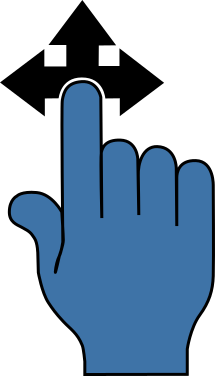
\includegraphics[width=0.7cm]{figures/gesture.pdf}}}}

% Define command to insert specific gesture image
\newcommand{\gesturespec}[1]{\marginlabel{\parbox{1.3cm}{\includegraphics[width=0.9cm]{figures/#1.png}}}}

% Define command to insert warning image
\newcommand{\warning}[0]{\marginlabel{\parbox{1.3cm}{
\includegraphics[width=0.9cm]{figures/warning.pdf}}}}

% Define command to insert Achtung image
\newcommand{\achtung}[0]{\marginlabel{\parbox{1.3cm}{
\includegraphics[width=2.5em]{figures/warning.pdf}}}}

% Define command to insert a flash image
\newcommand{\blitz}[0]{\marginlabel{\parbox{1.3cm}{
\includegraphics[height=2.0em]{figures/reminder.pdf}}}}

% Define command to insert a stop
\newcommand{\halt}[0]{\marginlabel{\parbox{1.3cm}{
\includegraphics[height=2.0em]{figures/warning.pdf}}}}

% Define command to reference a configuration item
\newcommand{\config}[1]{\marginlabel{\ref{conf:#1}
\parbox{1.3cm}{
\includegraphics[width=0.8cm]{figures/config.pdf}}}}

% Define command to draw a sketch on the margin
\newcommand{\sketch}[1]{\marginpar{\parbox{4.0cm}{\includegraphics[angle=0,width=1.0\linewidth,keepaspectratio='true']{#1}}}}
\newcommand{\smallsketch}[1]{\marginpar{\includegraphics[angle=0,keepaspectratio='true']{#1}}}


% Potentially overdue ``InfoBox'' style macro
\newcommand{\InfoBox}[0]{{InfoBox}}

% Enumerated todo's for the todonotes package
\newcounter{todocounter}
\newcommand{\todonum}[2][]{\stepcounter{todocounter}\todo[#1]{\thetodocounter: #2}}

\maxipagerulefalse

% Include XCSoar header and footer settings
\usepackage{calc}

% Colors
\definecolor{buttongray}{rgb}{0.831,0.816,0.784}


% A set of boxes, buttons etc.
%
% Simple gray button
\newcommand{\blink}[0]{$\triangleright$}

\newcommand{\bmenug}[1]{
  \fcolorbox {black}{buttongray}{{\footnotesize\textsf{#1}}}
}

\newcommand{\button}{\bmenug}
\newcommand{\bmenu}{\bmenug}

\newcommand{\bmenuw}[1]{
  \fcolorbox {black}{white}{{\footnotesize\textsf{#1}}}
}

\newcounter{mboxwidth}
\setcounter{mboxwidth}{14}
\newcommand{\setbuttonwidth}[1]{\setcounter{mboxwidth}{#1}}

\newcommand{\bmenut}[2]{    % Menu button (two lined)
  \fcolorbox {black}{buttongray}{
    \makebox[\value{mboxwidth}mm][c]{
      \begin{tabular}{c}
        {\footnotesize\textsf{#1}}\\
        {\footnotesize\textsf{#2}}
      \end{tabular}
    }
  }
}

\newcommand{\bmenuth}[3]{    % Menu button (three lined)
  \fcolorbox {black}{buttongray}{
    \makebox[\value{mboxwidth}mm][c]{
      \begin{tabular}{c}
        {\footnotesize\textsf{#1}}\\
        {\footnotesize\textsf{#2}}\\
        {\footnotesize\textsf{#3}}
      \end{tabular}
    }
  }
}

\newcommand{\bmenus}[1]{    % Menu button (single line)
  \fcolorbox {black}{buttongray}{
    \makebox[\value{mboxwidth}mm][c]{
      \begin{tabular}{c}
        {\footnotesize\textsf{#1}}\\
        \\
      \end{tabular}
    }
  }
}

\newcommand{\infobox}[1]{    % Normal Info box in text
  \fcolorbox {black}{white}{\makebox[1.7cm][c]{\textsf\strut #1}}
}

% Some more convenience
\newenvironment{jspecs}{ % Description spacing
  \itemsep=2pt\topsep=3pt\partopsep=3pt\parskip=0pt
  \begin{description}
    \itemsep=2pt\topsep=3pt\partopsep=3pt\parskip=0pt
}{\end{description}}

\newcommand{\jindent}[2]{ % Extra list spacing
  \noindent\makebox[0pt][r]{{#1}\hspace*{\marginparsep}}
  \parbox[t]{0.95\linewidth}{#2}\par
}

\widowpenalty=1000
\clubpenalty=1000

% the command \version prints the XCSoar version number
\newcommand{\version}{\begingroup\catcode`\_=\active\input{VERSION.txt}\endgroup}

% Define command to put a menu label on the margin
% aligned left
\newcommand{\menulabel}[1]{\marginpar{\parbox{5.0cm}{\raggedright #1}}}
% aligned right
\newcommand{\menulabelr}[1]{\marginpar{\parbox{4.05cm}{\raggedleft #1}}}

% Define some colors
\definecolor{AirspaceYellow}{rgb}{.99,.99,.19}
\definecolor{AirspaceRed}{rgb}{.99,.19,.19}


\title{Manuel de l'utilisateur}


% Set the page title
\usepackage{calc}
\usepackage{fancyhdr}

\newcommand{\xcsoarheader}[1]{
  \pagestyle{fancy}

  % Add XCSoar User Manual title to the header
  \fancyhead[L]{\hspace*{-\marginparsep}\hspace*{-\marginparwidth}\em#1}

  % Add page number to the footer (centered)
  \fancyfoot{}
  \fancyfoot[R]{\thepage}
}

% No line between content and header
\renewcommand{\headrulewidth}{0pt}

\fancypagestyle{plain}{
  % Clear fancy header and footer
  \fancyhf{}

  % Add page number to the footer (centered)
  \fancyfoot[R]{\thepage}

  % No line between content and header
  \renewcommand{\headrulewidth}{0pt}
}

\xcsoarheader{XCSoar: Manuel de l'utilisateur}

\def\maketitle{%
  \null
  \thispagestyle{empty}%
  \begin{maxipage}
    \begin{center}
    
\includegraphics[angle=0,width=0.5\textwidth,keepaspectratio='true']{graphics/logo.png}
    \vskip 0.5cm
    
\includegraphics[angle=0,width=0.66\textwidth,keepaspectratio='true']{graphics/title.pdf}
    \end{center}
    \begin{center}
      \normalfont\huge\textsf{La Navigation Open Source}\par
    \end{center}
    \vskip 1cm
    \begin{center}
      \normalfont\huge\textsf{\@title}\par
    \end{center}
    \vskip 1cm
  \end{maxipage}

  \vfill
  \todo[nolist,size=\Large,inline]{Traduction en cours, vérifiez qu'il n'y a pas de version plus récente avant d'imprimer.}

  \begin{flushright}
    \large \strut {
      \sf
      \today \\
      XCSoar version \version \\
      \xcsoarwebsite{} \\
    } 
    \par
  \end{flushright}
  \par
  \vfil
  \vfil
  \null
  \cleardoublepage
}

\usepackage{xkeyval}
\usepackage{framed}
\usepackage{babel}
\begin{document}
\maketitle

%%%%%%%%%%%%%%%%%%%%%%
\listoftodos

%cela est toujours le cas quand le Goto automatique existe ???
%\tip It is also possible to save a `default' task and have this task loaded
%automatically upon start-up of XCSoar.  One application of this is to
%set up a default task with one waypoint being the home --- this means
%that XCSoar is then programmed for final glide back to home, which is
%useful for casual cross-country touring.


\warning 
CE MANUEL EST EN COURS DE TRADUCTION! 
IL N'EST PAS VRAIMENT UTILE ET TRÈS ÉCOLOGIQUE DE L'IMPRIMER VU QU'IL VA ENCORE BEAUCOUP ÉVOLUER ET QU'IL RESTE PAS MAL DE TEXTE EN ANGLAIS.
IL PEUT AUSSI CONTENIR DES ERREURS!!!
POUR SIGNALER CE GENRE DE CHOSES... VOUS POUVEZ CONTACTER Daniel: osteocool@yahoo.fr

MERCI
%%%%%%%%%%%%%%%%%%%%%%
\begingroup
\setlength{\cftsecnumwidth}{3em}
\tableofcontents
\endgroup


%%%%%%%%%%%%%%%%%%%%%%
\chapter*{Préface}

\section*{Avertissements et précautions d'utilisation}

\warning IL EST DE LA RESPONSABILITÉ DE L'UTILISATEUR D'UTILISER CE LOGICIEL AVEC LA PLUS GRANDE PRUDENCE. CE LOGICIEL EST DESTINE A ETRE UTILISE UNIQUEMENT COMME UNE AIDE A LA NAVIGATION ET NE DOIT PAS ÊTRE UTILISÉ DANS LES CAS EXIGEANT UNE MESURE PRECISE DU CAP,DE LA DISTANCE, DE LA POSITION OU DE LA TOPOGRAPHIE. CE LOGICIEL NE DOIT PAS ÊTRE UTILISÉ COMME AIDE POUR DÉTERMINER L’ALTITUDE EN NAVIGATION AERIENNE. CE LOGICIEL NE DOIT PAS ÊTRE UTILISÉ COMME UN SYSTEME ANTI\-COLLISION.

\section*{Mentions légales}

\subsection*{Contrat de licence logicielle}

Ce logiciel est distribué conformément à la licence GNU « General Public License » Version~3. Voir l'annexe (~\ref{cha:gnu-general-public}) pour le texte complet de l’accord de licence et des provisions de garantie.

\subsection*{Limitation de responsabilité}

En aucun cas, XCSoar, ses dirigeants, actionnaires, cadres, employés, sociétés affiliées, sous-traitants, filiales, ne peuvent être tenues responsables des dommages accessoires, indirects ou dommages-intérêts punitifs de toute nature, suite à l'utilisation du produit.

\subsection*{Avertissement}

Ce produit, et tous les fichiers joints, données ou documents, sont distribués «tels quels» et sans garantie d'aucune sorte, expresse ou implicite. Ce produit est utilisé entièrement sous la responsabilité de l'utilisateur. Bien qu'un grand soin ait été pris pour identifier les éventuelles erreurs pendant
le développement, il n’est en aucun cas revendiqué comme exempt de tout défaut . Aucune garantie n’est fournie quant à son exactitude, sa fiabilité ou son adéquation à un besoin particulier. Les développeurs  et les contributeurs du projet XCSoar ne peuvent en aucun cas être tenu responsables des erreurs pouvant s’y trouver ou des dommages fortuits ou consécutifs, de toute perte de données ou de tout dommages corporels pouvant survenir dans le cadre de la livraison, de la mise en service ou de l'utilisation de ce programme.


%%%%%%%%%%%%%%%%%%%%%%
\chapter{Introduction}\label{cha:introduction}
This document is a pilot's manual for XCSoar, an open-source glide
computer originally developed for Pocket PC devices.  The audience 
is assumed to have a sound knowledge of the fundamental theory of flight for
gliders, and at least a basic working knowledge of cross-country soaring.

Updates to the XCSoar software may result in some of this manual being
out of date. You should read the release notes distributed with the
software to keep track of changes.  Updates to the manual and software
are available from 
\begin{quote}
\xcsoarwebsite{}
\end{quote}

\section{Organization of this manual}

\todonum[inline]{Write about the manual crossref hinting icons and the yellow
colour. The Quickstart will be readable also without those links available} 
This manual most notably is written in order to get the XCSoar user started 
quickly  \emph{as well as} support his deep understanding of all the features, 
concepts and tactics introduced. At all times, the authors made their effort 
for doing this from a pilot's perspective (and honestly hope for having 
succeeded).

The authors highly encourage you to take your time reading the entire manual 
chapter by chapter (with exception of the reference chapters Infoboxes and 
Configuration). Feel assured, the time you will have spent will pay off as a 
manifold in understanding. On your way reading you might feel blue once in a 
while. That is why the authors introduced some blueish things: links and 
icons.

\begin{figure}[h]
\centering

\includegraphics[width=0.8cm,angle=0,keepaspectratio='true']{figures/config.pdf}
\hspace{1.5cm}

\includegraphics[width=0.8cm,angle=0,keepaspectratio='true']{figures/reminder.pdf}
\hspace{1.5cm}
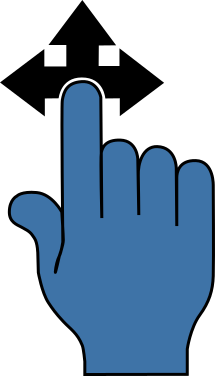
\includegraphics[width=0.8cm,angle=0,keepaspectratio='true']{figures/gesture.pdf}
\hspace{1.5cm}

\includegraphics[width=0.8cm,angle=0,keepaspectratio='true']{figures/warning.pdf}
\caption{Icons configuration, reminder, gesture, warning}
\end{figure}

\warning Warning. The icon warning is used, whenever things shall be followed 
strictly.  Not following will cause unexpected results, total dysfunction, or
even danger to life. Proceed only, if warning understood.

\gesture{DU} Gesture. A swipe gesture input is available using devices with a 
touch screen to invoke a menu or function amongst others. In this example, DU 
stands for moving your fingertip down, then up, (in straight lines) on the 
screen.
  
\gesturespec{du} Specific Gesture. Whenever the manual's authors kept up with XCSoar's rapid development process
in writing, a specific icon is provided, depicting the movements.

\tip Reminder. This icon tags a tip, trick, things you might remind after having read corresponding sections and so on.

\config{orientation} Configuration see... The icon depicting two craftsman's
tools refers to an in-depth description of items being mentioned and how to 
configure them. The numbers beside the icon refer to a specific chapter / 
section of this manual's reference chapters \ref{cha:infobox} and 
\ref{cha:configuration}, in this case referring to section 
\ref{conf:orientation}. 

\marginlabel{\parbox{1.3cm}{\rotatebox[origin=c]{180}{
\includegraphics[width=0.9cm]{figures/warning.pdf}}}}
\rotatebox[origin=c]{180}{Stop from reading manuals whilst flying inverted!}

\emph{Read} at home, \emph{configure} on the ground, safely. Having perceived 
this (inverted) warning as an example, you are ready to proceed.

\config{usingxcsoarsafely} Referring to the second exemplary case of the icon 
``configuration'' to the left, the icon points
towards chapter \ref{cha:introduction}, (this chapter), section 
\ref{sec:usingxcsoarsafely}, ``Using XCSoar safely'' underneath, which could be
understood as a ``how to configure yourself''. It is up to you whether to jump
to an in depth discussion and go back or just proceed. If reading this manual 
electronically, clicking the number will let you jump to the requested cross
-reference.  Use the go-to ``back'' (or similar) function of your particular
browser to proceed with the chapter you jumped from.

The numbers are printed in blue as are the icons introduced, signalling ``help
available''. And so are other Universal Resource Locators, underlying blue
text. Clicking on text like \xcsoarwebsite{/contact} will open your world wide 
web browser or mailer to get in touch with other resources or knowledgeable
people respectively.

The remainder of this chapter ``Introduction'' is about getting you prepared for
XCSoar, how to raise your level of understanding and maintain your skills. 
Chapter \ref{cha:quickstart} ``Quickstart'' might be the next waypoint after
\ref{cha:installation} ``Installation'' for the urgent user. Feel free to cut
short, but do not resume too sadly when reading chapter by chapter, following:

Chapter~\ref{cha:interface} introduces the user interface
concepts and gives an overview of the display .

Chapter~\ref{cha:navigation} describes the moving map part of the
display in greater detail and describes how the software can assist in
general navigation.  Chapter~\ref{cha:tasks} describes how
cross-country tasks are specified and flown, and presents some of the
analysis tools available to pilots to help improve their performance.
Chapter~\ref{cha:glide} goes into further detail on the glide computer
functions as it is important for pilots to be aware of how the
computer performs its calculations.

Chapter~\ref{cha:atmosph} describes how the computer can interface to
variometers and other air data sensors, and how it uses these
measurements to provide various models of the atmosphere, in
particular on winds and thermal convection.
Chapter~\ref{cha:airspace} describes how XCSoar can assist in managing
flight in special use airspace and the FLARM collision awareness
system.  Chapter~\ref{cha:avionics-airframe} deals with systems
integration and systems diagnostics, the integration of XCSoar with
communications devices and with airframe switches.

The remainder of the manual contains mainly reference material.
Chapter~\ref{cha:infobox} lists the types of information that can be
displayed in the grid of InfoBoxes next to the map display.  The
configuration of the software is described in detail in
Chapter~\ref{cha:configuration}.  The formats of the various data
files that program uses, as well as where to obtain them from and how
to edit them, is described in Chapter~\ref{cha:data-files}.

Finally, a short history and discussion of XCSoar's development
process is presented in Chapter~\ref{cha:history-development}.

\section{Notes}

\subsection*{Screenshots}
Throughout this manual are several screenshots of XCSoar. These are
taken from the program running on a variety of hardware platforms and possibly
even different versions. Each platform and version may have different screen
resolutions, layouts and fonts, and so there may be slight differences in the
appearance of the display. Most of the screenshots in this manual are taken of
XCSoar running in landscape orientation.

\section{Platforms}
\begin{description}
\item[Android Devices]
XCSoar runs on Android 1.6 or newer.
\item [eBookreader]
XCSoar runs on several Kobo eReader devices.
\item[Windows PC]
It is possible to run XCSoar on an ordinary computer with the Windows
operating system (Vista and above). This setup can be used for training yourself in using XCSoar.
A simulation mode is included in XCSoar as well as a IGC replay function, that
can be used when not connected to a valid GPS source.
\item[Unix/Linux PC]
XCSoar runs on Unix/Linux.
\end{description}



\section{Technical support}

\subsection*{Troubleshooting}
A small team of dedicated developers produces XCSoar. Although we are
happy to help with the use of our software, we cannot teach you about
basics of modern information technology. If you have a question about XCSoar in
particular not found in this manual please get in touch. You will find all of the following links summarized at:
\begin{quote}
\xcsoarwebsite{/contact}
\end{quote}
To begin with communication, join the XCSoar forum at:
\begin{quote}
\url{https://forum.xcsoar.org}
\end{quote}
If your concern appears not already addressed, post it or email us: 
\begin{quote}
\href{mailto:xcsoar-user@lists.sourceforge.net}{xcsoar-user@lists.sourceforge.net}
\end{quote}
Any frequent questions will be added to this document.
You may also find it useful to subscribe to the XCSoar users mailing
list so you will be kept up to date with latest developments.

If all of this does not help, you probably discovered a bug.

\subsection*{Feedback}
Like any complex software program, XCSoar may be subject to software
bugs, so if you find any, please report them to the XCSoar developers
by using our bug tracker portal at: 
\begin{quote}
\xcsoarwebsite{/develop/new_ticket.html}
\end{quote}
or by sending an email to
\begin{quote}
\href{mailto:xcsoar-devel@lists.sourceforge.net}{xcsoar-devel@lists.sourceforge.net}
\end{quote}
XCSoar logs many valuable things in a logfile
\verb|xcsoar.log| in the \texttt{XCSoarData} directory. The logfile can be appended to the bug ticket in order to help XCSoar developers determine the cause of possible problems.
If you like the idea of doing some more, get involved:
\begin{quote}
\xcsoarwebsite{/develop}
\end{quote}

\subsection*{Updates}
You should periodically visit the XCSoar website to check for program
updates. The installation procedure in the following chapter can typically be
repeated in order to upgrade the software.  All user configuration
settings and data files will be preserved during the
re-installation/upgrade.

It is also recommended to periodically check for updates to data
files, particularly Special Use Airspace, which may be subject to
change by the national civil aviation authority.

\section{Training}
For the safety of yourself and others, pilots using XCSoar are advised to
train themselves in using XCSoar on the ground and become familiar with its
interface and features prior to flight.

\subsection*{Using XCSoar on the PC}
The PC versions of XCSoar may be used to become familiar with XCSoar's
interface and functionality in the comfort of one's home.  All files
and configuration used by this version are identical to the embedded versions,
so it can be helpful to try out customisations on the PC version before using
them in flight.

The PC versions can also be connected to external devices and operate just as
the embedded versions do. Suggested uses include:
\begin{itemize}
\item Connect the PC to a FLARM device to use XCSoar as a ground
station display of FLARM-equipped traffic.
\item Connect the PC to an intelligent variometer such as Vega to
test configuration settings of the variometer.
\end{itemize}

\subsection*{Using XCSoar with a flight simulator}
A good way to learn how to use XCSoar is to connect the smartphone
device to a PC running a flight simulator that can output NMEA
sentences to the serial port. Suitable simulators include Condor and
X-Plane.  

The benefit of this form of training is that XCSoar can be used in FLY
mode, so it behaves exactly as if you were really flying, and you can
get a good feel for how the program works while you are flying the
simulator.

\section{Using XCSoar safely}\label{sec:usingxcsoarsafely}\label{conf:usingxcsoarsafely}
The use of an interactive system like XCSoar in flight carries with it
certain risks due to the potential distraction of the pilot from
maintaining situational awareness and eyes outside the cockpit.

The philosophy guiding the design and development of the software is
to try to reduce this distraction by minimising the need for user
interactions as much as possible, and by presenting information in a
clear fashion able to be interpreted at a glance.

Pilots using XCSoar must take responsibility for using the system safely.
Good practice in the use of XCSoar includes:
\begin{itemize}
\item Becoming familiar with the system thoroughly through training on 
  the ground.
\item Performing clearing turns before interacting with XCSoar in flight
  in order to ensure there is no collision risk with other traffic.
\item Setting up the system to take advantage of automatic functions
  and input events so that user interactions can be minimised.  If you
  find yourself mechanically performing certain interactions frequently,
  ask yourself (or other XCSoar users) if the software can be made to do 
  these interactions for you.
\end{itemize}

% !TeX encoding = utf8
% !TeX spellcheck = fr

\chapter{Installation}\label{cha:installation}

Pour lancer XCSoar il vous faut~:
\begin{itemize}
\item un appareil sur lequel faire tourner XCSoar
\item le logiciel XCSoar
\item un récepteur GPS (peut être dans l'appareil)
\item un fichier de points de virage
\item un fichier d'espaces aériens (optionnel)
\item un fichier de terrain, pour la carte (optionnel)
\end{itemize}

\section{!~Avant de faire votre premier vol avec XCSoar~!}

Après avoir installé XCSoar avec succès, vous pourriez l'utiliser directement. XCSoar
démarrera avec une pré-configuration prête à être utilisée. Mais attention qu'à 
ce moment-là votre nouveau jouet ne vous affichera qu'une carte mobile.
\warning \emph{Ne faites pas confiance aux calculs.} Il faut dire à l'avance à XCsoar sur quel
aéronef vous volez. Ceci est fait en précisant les données sur votre aéronef
telles que la polaire, sa masse et d'autres données. Cependant, il est toujours bon
d'étudier le manuel et de se familiariser avec XCSoar à la maison.

\section{Comment tirer le maximum d'XCSoar}

Afin de bénéficier au maximum d'XCSoar, il vous est demandé de
faire des choses supplémentaires après l'installation du logiciel et de télécharger quelques fichiers
de données. ``Des choses supplémentaires'' incluent des données personnelles et sur l'aéronef, ainsi que la configuration
de quelques fonctionnalités. A moins que vous souhaitiez peaufiner tout ce que XCSoar
fournit, cela peut se faire assez rapidement. Les étapes nécessaires sont
résumées dans une \emph{Checklist d'XCSoar}, fournit dans le paragraphe suivant.

Si vous comptez utiliser un appareil avec plusieurs composants connectés,
ce manuel vous donnera des conseils utiles à la fois sur la configuration des choses et sur
leur utilisation.

Si vous êtes un pilote pressé, les auteurs vous suggère d'aller voir la version courte
du manuel \texttt{XCSoar-Prise-en-main} et de parcourir la \emph{Checklist d'XCSoar}
étape par étape. La version courte du manuel est disponible sur \xcsoarwebsite{/discover/manual.html}.

\section{Checklist d'XCSoar}

\subsection*{{Mise en piste d'XCSoar}}
\begin{itemize}
\item acquérir un appareil et y installer XCSoar
\item récupérer les fichiers de données adapté à votre secteur de vol
\item dire à XCSoar quels fichiers utiliser
\item dire à XCSoar la polaire et la masse de votre planeur
\item éventuellement, se connecter aux instruments
\item terminer la configuration et se familiariser
\item monter l'appareil
\item ajouter les points listés ci-dessous dans vos checklists
\item définir le point de départ
\end{itemize}

\subsection*{Faire les vérifications pré-vols, incluant~:}
\begin{itemize}
\item configurer la polaire et la masse
\item configurer le vent et les paramètres de vol (MC, moucherons, QNH)
\item éventuellement, configurer un circuit.
\end{itemize}

\subsection*{Faire les vérifications avant le décollage, incluant~:}
\begin{itemize}
\item vérifier le vent et la configuration de vol une fois de plus
\end{itemize}
\vspace{2em}

\subsection*{Voler, prendre du plaisir}
\vspace{4em}

\subsection*{Faire les vérification post-vol}
\begin{itemize}
\item Télécharger les logs du vol depuis l'enregistreur, les mettre sur skylines, la netcoupe et l'OLC
\item Récupérer les données statistiques sur le vol.
\end{itemize}
\newpage

\section{Compatibilité}

\subsection*{Appareils faisant tourner XCSoar}

XCSoar tourne sur les plateformes suivantes~:
\begin{itemize}
\item téléphones portables et tablettes sous Android 1.6 ou plus récent \\
 Exemples~: Dell Streak, Samsung Galaxy S II, HTC Desire HD,
 Motorola Xoom
\item eReader Kobo
\item Windows 2000 ou plus récent
\item Linux
\item Mac OS X (obsolète)
\end{itemize}

\subsection*{GPS, Enregistreur de Vol, Vario}

XCSoar est compatible avec tous les GPS fournissant des données NMEA. La plupart
des appareils Android intègre un GPS, mais, pour diverses raisons, il est désirable de
se connecter à un ou plusieurs appareils externes~:
\begin{itemize}
\item un récepteur GPS spécialisé possède une bien meilleure réception, fournissant de bien
meilleures données pour les mesures et les calculs
\item un indicateur de vitesse fournit de manière exacte et rapide des estimations du vent
 sans nécessiter de spiraler
\item un variomètre améliore l'assistant en thermique
\item un circuit peut être déclaré dans un enregistreur de vol IGC et, après l'atterrissage, l'enregistrement
du vol peut être téléchargé
\item certains variomètres permettent la synchronisation de la configuration du MacCready avec
 XCSoar
\item un FLARM (voire une entrée ADS-B) fournit des informations et des états sur les autres
autour de vous (et bien sûr, un FLARM détecte des risques de collision)
\end{itemize}

\subsection*{Appareils externes compatibles et fonctionnalités}
\label{sec:supported-varios}

\newcommand{\y}[0]{{ $\surd$ }}
%{0.8\textwidth}
\noindent\makebox[\textwidth]{%
\begin{tabular}{l|ccc|cc|cc|c}
    \multicolumn{1}{c}{Compatibles} & \multicolumn{3}{c|}{Fonctionnalités} & \multicolumn{5}{c}{Flux de données} \\
NMEA Device & 
 \begin{sideways} Déclaration\end{sideways} & 
 \begin{sideways} Télécommande\end{sideways} & 
 \begin{sideways} Téléchargement\end{sideways} &
 \begin{sideways} Vitesse air\end{sideways} & 
 \begin{sideways} Vario\end{sideways} & 
 \begin{sideways} Baro.\ altitude\end{sideways} &
 \begin{sideways} Vent\end{sideways} &
 \begin{sideways} Accéléromètre\end{sideways} \\
\hline
%                    _Decl_Remo_Down_Airs_Vari_Baro_Wind_Gsen_
Borgelt B50          &    & \y &    & \y & \y & \y &    &    \\
CAI 302              & \y & \y & \y & \y & \y & \y & \y & \y \\
CAI GPS Nav          &    &    &    &    &    &    &    &    \\
Condor               &    &    &    & \y & \y & \y & \y &    \\
\hline
Digifly Leonardo     &    &    &    & \y & \y & \y & \y &    \\
EW Logger            & \y &    &    &    &    & \y &    &    \\
EW microRecorder     & \y &    &    &    &    & \y &    &    \\
FLARM                & \y &   & \y  &    &    & \y &    &    \\
\hline
%                    _Decl_Remo_Down_Airs_Vari_Baro_Wind_Gsen_
Flymaster F1         &    &    &    &    & \y & \y &    &    \\
Flytec 5030          &    &    &    & \y & \y &    &    &    \\
ILEC SN10            &    &    &    &    & \y & \y & \y &    \\
\hline
IMI ERIXX            & \y &    & \y &    &    &    &    &    \\
LX20, Colibri        & \y &    & \y &    &    & \y &    &    \\
LXNAV Nano           & \y &    & \y &    &    &    &    &    \\
\hline
%                    _Decl_Remo_Down_Airs_Vari_Baro_Wind_Gsen_
LXNAV V7             &    & \y &    & \y & \y &    &    &    \\
PosiGraph            & \y &    &    &    &    & \y &    &    \\
Triadis Altair (pro) & \y &    &    &    &    & \y &    &    \\
Triadis Vega         &    & \y &    & \y & \y & \y &    & \y \\
\hline
Vaulter              &    & \y &    & \y & \y & \y & \y & \y \\
Volkslogger          & \y &    & \y &    &    & \y &    &    \\
Westerboer VW1150    &    & \y &    & \y & \y & \y &    &    \\
XCVario              &    & \y &    & \y & \y & \y & \y & \y \\
Zander / SDI         &    & \y &    & \y & \y & \y & \y &    \\

\end{tabular}}

Alors que la majorité des appareils sous Windows CD ont un port série, des matériels
aussi anciens ne sont pas présent sur les appareils Android modernes. Ces derniers peuvent soit
utiliser le Bluetooth ou une carte Android IOIO. Pour utiliser le Bluetooth, vous devez
connecter le périphérique externes à un adaptateur Bluetooth-vers-Série, tels
que le K6-Bt et le SoarTronic-BT1/2.

\section{Installation du logiciel}

Le logiciel est téléchargeable gratuitement sur le site internet d'XCSoar ~\xcsoarwebsite{}. Ce paragraphe décrit quel fichier doit être téléchargé, et comment l'installer.

\subsection*{Sous Android}

Récupérez XCSoar sur Google Play depuis votre appareil, ou installez le fichier \verb|apk|
manuellement. Copiez les fichiers de données sur la carte SD dans le répertoire \verb|XCSoarData|.

\subsection*{Sur un Kobo Mini}

Le Kobo Mini est un lecteur d'e-book pas cher. Il a un affichage
e-paper noir et blanc qui possède une excellente lisibilité en plein soleil.

Avant de commencer, faites une sauvegarde de la carte SD interne. L'installateur d'XCSoar
pourrait casser votre Kobo, quoi que ce soit improbable. Vous pouvez toujours récupérer le Kobo
d'une défaillance logicielle, mais uniquement si vous avez accès à une sauvegarde.

Pour installer XCSoar, connecter par USB le Kobo à votre PC. Le Kobo 
apparaît comme un périphérique de stockage sur votre PC~; ouvrez-le et créer un
répertoire nommé \texttt{.kobo} (noter le point initial). Téléchargez le 
fichier \texttt{KoboRoot.tgz} depuis le site internet d'XCSoar vers ce
répertoire (\xcsoarwebsite{/hardware/}). Débrancher le Kobo et le redémarrer (arrêter le complètement
puis allumer le à nouveau). Vous verrez le message ``Updating'' (``mise à jour'') et
après quelques minutes, le Kobo affichera un menu qui vous permet de lancer
XCSoar ou le logiciel de lecteur d'\mbox{e-book} du Kobo.

Pour copier les fichiers de données (cartes, points de virage...) sur le Kobo, lancer le 
logiciel original du Kobo (``Nickel'') et connecter de nouveau le Kobo à votre PC.
Copier les fichiers dans un répertoire nommé \texttt{XCSoarData} à la racine.

Autrement, des fichiers de données peuvent être téléchargés depuis le gestionnaire de fichiers d'XCSoar,
en ayant démarré une connexion réseau avant le lancement d'XCSoar.

\subsubsection{Bidouiller le Kobo}

Suite à l'installation d'XCSoar sur le Kobo, le nouveau script de démarrage vérifie qu'un
script nommé \texttt{XCSoarData/kobo/init.sh} existe et le lance. Si
vous vous y connaissez, vous pouvez utiliser ce script pour effectuer des choses au
moment du démarrage, comme lancer \texttt{inetd} (pour un accès \texttt{telnet}).

Quand vous lancer \texttt{Nickel} (le système original de l'e-book), le nouveau
script de démarrage cherche aussi un script nommé \texttt{init\_nickel.sh}
dans \texttt{XCSoarData/kobo/} et le lance. Là aussi, si 
vous vous y connaissez vous pouvez utiliser ce script pour effectuer des choses
avant que \texttt{Nickel} n'est complètement démarré, comme envoyer des instructions
à votre vario apparié (pour l'éteindre, pour baisser le volume, etc.).

\subsection*{Sur un PC sous Windows}

Téléchargez le fichier programme \verb|XCSoar.exe| (cible ``PC'') sur votre disque dur.

\subsection*{Sous Unix/Linux}

Téléchargez \verb|xcsoar_XXX.deb|, où \verb|XXX| contient les numéros de version et la plateforme, par~ex.\ \verb|xcsoar_6.0.4_i386.deb|.
Il s'agit d'un paquet Debian et peut être installé ainsi 
\begin{center}
\verb|sudo dpkg -i xcsoar_XXX.deb|.
\end{center}
Utilisez \verb|dpkg-query -L xcsoar| pour voir où l'exécutable et les autres fichiers sont installés.
Les fichiers additionnels doivent être placés dans le répertoire
\verb|~/.xcsoar/|.
Si \verb|~/.xcsoar| n'existe pas, il sera créé la première fois que \verb|xcsoar| sera exécuté.

\subsection*{Sur une Raspberry Pi et une Cubieboard}

Installer le paquetage Debian tel que décrit ci-dessous. Toutefois, contrairement à 
Linux ``normal'', XCSoar n'utilisera pas X11. À la place, il tournera
en mode plein écran dans une console Linux.

XCSoar a besoin d'accéder à vos périphériques d'entrée
(\texttt{/dev/input/event*}). Par défaut, seul \texttt{root} y
a accès. Pour passer outre, créez un fichier de configuration
\texttt{udev}, par ex. \texttt{/etc/udev/rules.d/99-input.rules}~:

\begin{verbatim*}
KERNEL=="event*", NAME="input/%k", MODE="660", GROUP="input"
\end{verbatim*}

Créez le groupe \texttt{input} et en rendre membre votre utilisateur~:

\begin{verbatim*}
groupadd input
adduser pi input
\end{verbatim*}

\section{Fichiers de données}\label{sec:data files}

Pour être capable d'utiliser les fonctionnalités avancées d'XCsoar, des fichiers de données supplémentaires, tels que
le relief, la topographie, des espaces aériens à usage particulier, des points de virage, etc.\, sont nécessaires. Les fichiers
qui peuvent être utilisés avec XCSoar sont décrits dans le chapitre~\ref{cha:data-files}.

Tous les fichiers de données doivent être copiés dans le répertoire 
\texttt{XCSoarData}. Ce répertoire doit être dans un endroit spécifique
de telle façon qu'XCSoar sache où rechercher des fichiers de données~:
\begin{description}
\item[PC sous Windows]
\texttt{XCSoarData} est dans votre répertoire personnel (``\texttt{Mes
Documents}'')
\item[Windows Mobile PDA/PNA]
S'il y a un répertoire nommé \texttt{XCSoarData} dans le même
répertoire que \texttt{XCSoar.exe}, alors celui-ci sera utilisé.
\texttt{XCSoarData} est sur une carte SD. Si il n'y a pas de carte SD, alors
XCSoar le cherchera dans \texttt{Mes Documents}.
\item[Unix/Linux]
Le répertoire s'appelle \verb|.xcsoar| dans le répertoire principal de l'utilisateur.
\item[Appareil Android]
\texttt{XCSoarData} est sur la carte SD.
\end{description}

XCSoar générera un certain nombre de fichiers supplémentaires lors de l'exécution. Ils
seront placés dans le répertoire \texttt{XCSoarData} (PS sous Windows, 
appareils mobiles sous Windows et Android), ou dans le répertoire \texttt{.xcsoar} (PC sous
Unix/Linux). Au moment du premier démarrage, XCSoar va créer et mettre à jour les fichiers
\texttt{user.cup} (points de virage édités par l'utilisateur),
\texttt{Default.tsk} (circuit par défaut), 
\texttt{default.prf} 
(paramètres de configuration),
\texttt{xcsoar.log}, 
ainsi que trois répertoires~: \texttt{cache},
\texttt{config} et \texttt{logs}. Des fichiers supplémentaires peuvent être 
créés/modifiés pendant que XCSoar tourne, tels que des fichiers de circuit
(\texttt{*.tsk}) et les enregistrements du vol.


\section{Faire tourner XCSoar}
%\subsection*{Fly and simulator modes}

Le logiciel XCSoar peut fonctionner selon deux modes~:
\begin{description}
\item[VOL] Ce mode est utilisé lorsque vous êtes vraiment en vol. Le simulateur est
 désactivé et les communications séries sont actives. 
\item[SIM] Cela lance XCSoar en mode simulateur, sans tenter de démarrer
 les communications séries.
\end{description}

\subsection*{Version PC de XCSoar}
Le logiciel peut être lancé en ouvrant la fenêtre de l'explorateur, en trouvant le répertoire
qui contient l'exécutable XCSoar.exe, et en double-cliquant sur le fichier du logiciel.

Les options en ligne de commande du logiciel permettent de définir
l'orientation de l'affichage~:
\begin{description}
\item[-portrait] L'écran fait 480~pixels de large, 640~pixels de haut.
\item[-square] L'écran fait 480~pixels de large, 480~pixels de haut.
\item[-landscape] L'écran fait 640~pixels de large, 480~pixels de haut. C'est la 
configuration par défaut. Si vous ne spécifier ce paramètre, la version paysage sera
chargé automatiquement.
\item[-small] Diminue la taille de l'écran de moitié. C'est utile pour se servir d'XCSoar en
même temps que de simulateurs de vol comme Condor.
\end{description}
Pour changer l'orientation de l'écran, il est pratique de créer un raccourci vers le
logiciel et, en faisant un clic droit sur l'icône du raccourci puis sur ``Propriétés''.
Dans le champ ``Cible'' ajouter l'option désirées parmi celles listées ci-dessus.

\subsection*{Version Unix/Linux de XCSoar}
Lancer \verb|xcsoar| à partir de la ligne de commande, ou créer un raccourci sur le 
bureau. La localisation du fichier exécutable peut être trouvé en utilisant
\verb|which xcsoar|. Pour le moment, seul le mode paysage est disponible.

\subsection*{Charger les fichiers de données}\label{sec:loaddatafiles}
La première fois qu'XCSoar est lancé, il ne charge pas automatiquement les
fichiers de données que vous avez placés dans le répertoire \verb|XCSoarData|. 
Pour dire à XCSoar quels fichiers charger double cliquer/tapoter la carte (la grande
surface blanche avec un symbole de planeur au centre),
Choisissez le menu \bmenug{Config 2} (cliquer/tapoter-le deux fois), puis sélectionne l'élément
\mbox{\bmenug{Système}.} L'écran de configuration devrait s'afficher~:
\sketch{figures/config-basic.png}
La première page vous permet de choisir les fichiers de carte,
de points de virage et d'espace aérien en cliquant/tapotant sur les zones de texte.
De nombreuses autres fonctionnalités d'XCSoar peuvent être ici configurées. Elles sont décrites en détails dans le
chapitre~\ref{cha:configuration}.
Une fois fait, XCSoar rechargera ces fichiers~: à partir de maintenant les fichiers de données
seront chargés automatiquement au démarrage. 

\subsection*{Démarrage et profils utilisateur}\label{sec:profiles}
Quand XCSoar démarre, il vérifiera les profils existants. Si plusieurs
profils sont détectés il affichera une petite fenêtre vous demandant quel profil
charger. Pour continuer, choisissez le profil désiré et appuyés sur Entrée. Si aucun
profil n'est choisi les paramètres de la session précédente seront chargés à nouveau. Des profils
peuvent être utiles dans les cas suivants~:
\begin{itemize}
\item différents pilotes
\item compétition ou vol de d'agrément
\item voler depuis différents endroits
\item différents aéronefs (avec différentes polaires)
\end{itemize}
Des profils peuvent aussi servir à conserver la sauvegarde d'une
configuration particulière. Presque tous les paramètres sont enregistrés dans un fichier
de profil avec l'extension \texttt{.prf}. Une fois que vous êtes satisfait de votre paramétrage,
faites deux copies de votre fichier de profil. Une première ayant l'extension \texttt{.prf}, 
une seconde avec l'extension \texttt{.bak}.
Alors que le fichier \texttt{.prf} se lancera au démarrage et contiendra tous 
vos changements depuis que XCSoar tourne jusqu'au prochain démarrage, le fichier
\texttt{.bak} préservera vos paramètres, tant que vous jugerez utile de le faire.
A titre d'exemple, vous pourriez créer une série de fichiers tels que~:
\begin{itemize}
\item \texttt{CopainsEnArcus.prf}
\item \texttt{CopainsEnArcus.bak}
\item \texttt{JohnEnKa6auPaysDesMerveilles.prf}
\item \texttt{JohnEnKa6auPaysDesMerveilles.bak}
\end{itemize}

\subsection*{Mode SIM}
XCSoar possède une interface simple permettant de faire un vol
simulé. Selon l'appareil utilisé, il y a différentes
méthodes pour modifier les valeurs de cap, de vitesse et de hauteur. La simulation est
prévue pour une première familiarisation avec XCSoar en action. Si vous appréciez
l'idée d'une simulation plus réaliste à la maison, vous devriez acquérir un ``vrai''
simulateur de vol plané, à connecter à XCSoar.

Sur l'écran de la carte, cliquer/toucher le symbole du planeur
et le déplacer crée un déplacement du planeur dans cette direction, la
vitesse étant proportionnelle à la longueur du déplacement.

Avec des boutons, la vitesse, l'altitude et le cap de l'aéronef
peuvent être changés en utilisant les Infoboxes.
Ce qui suit pourrait ne pas être complètement disponible sur tous les appareils, mais sur
tout appareil faisant tourner XCSoar, toutes les entrées nécessaires pour
réaliser une simulation existent.

En appuyant sur une Infoboxe vous sélectionnez une valeur à modifier avec des boutons
réels ou du menu.
L'altitude de l'aéronef peut être modifiées en sélectionnant l'Infoboxe
d'altitude GPS \bmenuw{Alt GPS}, puis en utilisant les touches haut et bas ou les boutons
de l'écran tactile.
La vitesse par rapport à l'air peut être modifiée en sélectionnant l'Infoboxe de vitesse sol
\bmenuw{V Sol}, puis en utilisant les touches haut et bas ou les boutons du menu.
La trace du planeur peut être modifiée en sélectionnant l'InfoBoxe de trace 
\bmenuw{Trace}, puis en utilisant les touches haut et bas ou les boutons du menu.

En ayant sélectionné soit \bmenuw{Alt GPS} soit \bmenuw{V Sol},
le cap du planeur peut être modifié en utilisant les touches gauche/droite.

Les autres commandes, boutons et menus fonctionnent de la même façon qu'en mode VOL.


\subsection*{Écran d'accueil}
Quand XCSoar démarre, s'éteint ou charge de gros fichiers tels que les espaces aériens,
les points de virage, le relief, etc., un écran de progression est affiché pendant que les données sont
en train d'être chargée. Cet écran a une barre de progression qui indique l'activité
de chargement des données, et une courte ligne de texte décrivant l'action en cours.

Cet écran affiche aussi les information sur la version du logiciel.

\subsection*{Quitter le logiciel}
Sur les versions PDA ou PC, XCSoar est éteint en utilisant le menu. Ce menu peut être
ouvert en double-cliquant sur la carte ou sur l'\InfoBox 
\begin{quote}
\bmenug{QUIT}
\end{quote}

Sur les versions PC, XCSoar peut aussi être fermé en cliquant sur l'icône de fermeture
de la fenêtre XCSoar.


%%%%%%%%%%%%%%%%%%%%%%
\chapter{Interface do Usuário}\label{cha:interface}
\begin{figure}[h]
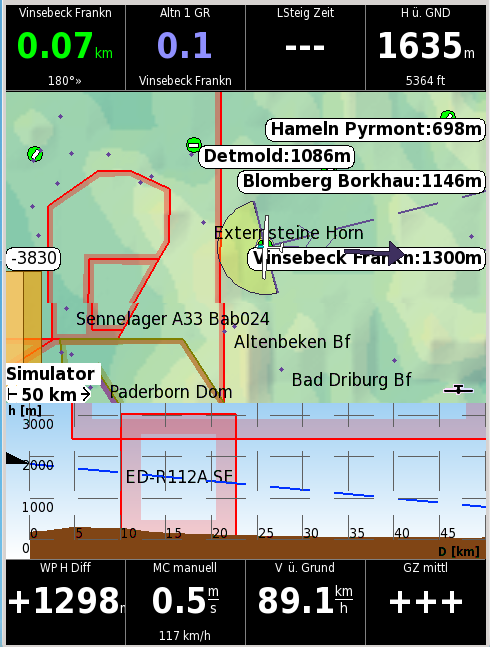
\includegraphics[angle=0,width=\linewidth,keepaspectratio='true']{figures/plain.png}
\caption{Layout mais comum da tela do XCSoar}
\end{figure}

Este capítulo descreve de um modo geral, os conceitos fundamentais da interface do usuário usados pelo XCSoar.  A tela principal mostra a maioria das informações necessárias para o vôo normal.   Geralmente a tela principal é composta de um mapa móvel e infoboxes.  Por várias razões – não é o escopo da introdução – você tem a oportunidade de utilizar várias telas principais, chamadas de páginas de telas.

As páginas de telas são facilmente acessadas por um gesto de deslizamento horizontal, como se tivesse virando páginas de um livro ou por um apertar de botão, dependendo do hardware que estiver usando.  Com a página de telas você estará apto a compor várias telas principais para tirar vantagem da sua utilização em diversas situações de vôo.  Simplificando, você poderá usar a informação apropriada em diferentes casos, podem ser acessadas muito facilmente e rapidamente.

Sempre que alguma situação que pode tirar a atenção do piloto, é mostrada uma informação na tela principal.  Isto acontece especialmente quando há a necessidade de reação do piloto, como uma possível colisão ou quando o piloto irá entrar em uma área de espaço aéreo restrito.

Evidentemente, os botões de menu e menu de telas também são sobrepostos à tela principal.  Como resultado, os elementos apresentados sobrepostos formam uma pilha de exibição com a tela principal representando a base.  As descrições mais detalhadas serão apresentadas nos capítulos seguintes. 


\section{Elementos exibidos}
\subsection*{Tela principal e página de telas}
Cada página de tela do conjunto de páginas do XCSoar é composta de várias partes:

\begin{description}
\item[Área principal] a grande parte da tela é normalmente dedicada à movimentação do mapa do GPS.  Vários símbolos relativos à informação de vôo são sobrepostas ao mapa.  Os ícones e textos devem aparecer ao longo da borda inferior da tela para indicar o estado dos dispositivos conectados, modos de vôo, etc.  De acordo com a evolução do desenvolvimento do XCSoar, há um aumento do número de itens que podem ser escolhidos para serem mostrados na área principal, como medidores FLARM, Radar, Assistente de Termal e Horizonte (como na versão 6.7.2, Dez. 2013).

\item[InfoBoxes] Uma grade de dados é mostrada na parte superior e inferior da tela (formato de retrato da tela), ou do lado direito da tela (formato de paisagem da tela).  São chamados de dados de infoboxes do GPS e outros dispositivos de entrada, bem como podem ter cálculos efetuados pelo XCSoar. Além disso, as Infoboxes podem mostrar também medidores e alguns gráficos.
\end{description}

\subsection*{Sobreposições}
\begin{description}
\item[Instrumentos]  os instrumentos mostram as medições dos sensores.  Todos os instrumentos são opcionais e alguns só poderão mostrar seus dados quando conectados aos dispositivos externos.  A sobreposição do instrumento na tela principal é permanentemente mostrada ou é somente mostrada em algumas condições críticas.  Ex. o assistente de termal é mostrado somente quando o XCSoar entra em modo de giro.  O radar FLARM é mostrado toda vez que há a possibilidade de colisão.  Os instrumentos permanentemente mostrados são a barra de planeio final, bem como a barra de variômetro, entre outros.

\item[Rótulos de Botões e Menus] Os botões do dispositivo que está rodando o XCSoar podem ser usados para navegar em pequenos menus na tela e são normalmente sobrepostos aos menus e podem ser selecionados apertando o botão deste item.  Se o dispositivo possui tela de toque, o item de menu pode ser selecionado clicando sobre o mesmo.  Estes botões são desenhados com texto preto em fundo cinza. 

\item[Mensagem de condição (estado)]o texto é mostrado sobre a tela em uma caixa de mensagens.  Este texto é utilizado para mostrar informações detalhados ao piloto quando alguns eventos ocorrem.

\item[Janela de diálogo] uma grande janela de diálogo, normalmente contendo gráficos e botões são usadas para mostrar dados detalhados ao piloto, relativos aos detalhes de waypoints, estatísticas e análises, etc.

\item[Menu principal] O menu principal é acessado clicando duas vezes na área do mapa ou infoboxes, bem como também por gesto.  Se o menu de botões não for pressionado após algum tempo, desaparecerá da tela para não obstruir a área do mapa. 
\end{description}

\subsection*{Mostrador de vário clássico}
Como dito acima, os mostradores podem ser mostrados de formas diferentes, em infoboxes, sobrepostos ou mesmo na área principal.  O mostrador do variômetro tradicional é diferente.  O mostrador em estilo agulha é mostrado permanentemente, escolhendo o layout da infobox que inclui o variômetro do lado direito das outras infoboxes.

\section{Interação}
Existem várias maneiras de interagir com o XCSoar:
\begin{itemize}
\item Tocando certos elementos no mapa
\item Tocando nas infoboxes e nos botões dos menus da tela.
\item 'Gesticulando', como por exemplo, desenhando um traço da esquerda para a direita na tela (veja seção  \ref{sec:gestures} abaixo).
\item ‘Arrastando’ a tela (tocando a tela e movendo antes de soltar).
\item Apertando os botões de função do dispositivo.
\item Apertando as teclas de cursor do dispositivo.
\item Apertando teclas ou chaves em um dispositivo conectado ao XCSoar.
\end{itemize}

Dependendo do dispositivo conectado ao XCSoar, nenhum destes métodos de interação são possíveis e podem haver números diferentes de funções dos botões.

Para a versão do XCSoar para PC, clicar com o mouse sobre um item tem a equivalência de tocá-lo.

Como o Altair não tem uma tela de toque, todas as interações do usuário são feitas através de botões físicos, chaves ou outro dispositivo conectado.  


\section{O menu principal de botões}
O menu de botões é um conjunto de botões mostrado na tela e ativado por toque ou botões físicos (quando houver no dispositivo).  Esta é a forma primária de interagir com o XCSoar.

\subsection*{A interface básica}
O menu é organizado em quatro grupos diferentes de funções, geralmente em forma de hierarquia.  O layout do menu depende da configuração de botões do hardware e plataforma, e podem também serem personalizados pelo usuário.

O XCSoar pode também aceitar entradas de teclados externos, gamepads, joysticks, etc.  Podem ser atribuídas às estas entradas uma grande variedade de funções.
\sketch{figures/buttonmenu.png}
Para o Altair, há quatro menus principais, ativados por um dos botões físicos verticais do lado esquerdo da tela.  Quando um menu é ativado, uma faixa de botões aparece na parte inferior da tela.  Apertando um botão do menu específico da tecla, irá entrar em várias páginas deste item.  Apertando o botão horizontal correspondente irá ativar o item.  Na última página, apertando o botão de menu novamente, irá desativar este menu e a faixa apresentada na tela desaparece.
Para a versão de PC, estes botões de modo são ativados pelas teclas 1, 2, 3 e 4.  As teclas 6, 7, 8, 9 e 0 correspondem à faixa horizontal de botões.

Na versão PDA, os botões de modo são ativados pelas teclas laterais do joystick.

Se o usuário não interagir com o computador por algum tempo, o menu será fechado automaticamente.  Seu tempo para fechamento é configurável.  A tecla “ESC” no PC ou PWR/ESC no Altair também pode ser utilizada para fechar o menu.

O menu de botões aparece acinzentado se a função correspondente não está disponível.  Por exemplo, se a lista de waypoints aparecer cinza, não há waypoints carregados.
Vários rótulos de botões tem o texto dinâmico baseado em seu contexto, de modo a tornar mais claro o que acontecerá se o botão for pressionado.  A convenção é usada para descrever o que acontecerá se o botão for pressionado. Por exemplo, se o botão descrever \bmenug{MC Auto},portanto, apertando o botão irá deixar o “Auto MacCready” e o texto do botão irá indicar \bmenug{MC Manual}. 
Neste menu descrito acima, são utilizados os rótulos genéricos. 

\subsection*{Menu de funções de grupo}
Esta seção descreve o layout padrão do sistema de menus em todas as plataformas.  As funções desempenhadas por cada botão são descritas com mais detalhes nos capítulos seguintes.

Os botões primários são ativados pelos botões na faixa vertical no Altair, do topo para baixo:

\begin{jspecs}
\item[\bmenug{Nav}] Ações para controle de navegação, provas simples de vôos de cross-country.
\item[\bmenug{Mostrar}]Ações para controle da tela.
\item[\bmenug{Config}] Configuração do XCSoar, dispositivos conectados e ajustes de vôo.
\item[\bmenug{Info}] Ativa várias janelas de diálogo de informações.
\end{jspecs}

Na versão para PC, as teclas 1, 2 3 e 4 ativam os menus correspondentes.  A lista de menus seguinte tem somente o lado esquerdo da maioria dos menus de botões e suas respectivas seções.  Siga-os para verificar todos os detalhes de cada um.

\section{Visão geral do Menu}

\subsection*{Menu de navegação}
\noindent\makebox[\textwidth]{%

\begin{tabularx}{1.44\textwidth}{c|ccccc}
\bmenus{Nav 1/2}
 & \bmenus{Prova}
 & \bmenut{Pto. virada}{Anterior}
 & \bmenut{Próx. Pto.}{Virada}
 & \bmenut{Lista}{Waypoint}
 & \bmenus{Alternativos} \\
veja
 & \ref{cha:tasks}
 & \ref{sec:advanc-rest-tasks}
 & \ref{sec:advanc-rest-tasks}
 & \ref{sec:waypoint-selector-dialog}
 & \ref{sec:alternates} \\ \\
\bmenus{Nav 2/2}
 & \bmenut{Prova}{Abortar}
 & \bmenut{Marcar}{Ponto}
 & \bmenus{Alvo}
 & {}
 & {} \\
veja
 & \ref{sec:taskabort}
 & \ref{sec:markers}
 & \ref{sec:waypointdetails}
\end{tabularx}}

Você não deve iniciar o uso do XCSoar sem antes saber sobre todas as características do “Alternativos”.  Qualquer “Prova” relacionada no menu de navegação é usada para planejar o vôo de cross-country e certamente será o segundo passo.

\subsection*{Menu Mostrar menu}
\noindent\makebox[\textwidth]{%

\begin{tabularx}{1.44\textwidth}{c|ccccc}
\bmenus{Mostrar 1/2}
 & \bmenut{Zoom}{In}
 & \bmenut{Zoom}{Out}
 & \bmenut{Zoom}{Auto}
 & \bmenut{Info}{Auto/...}
 & \bmenut{Pan}{On} \\
veja
 & \ref{sec:zooming}
 & \ref{sec:zooming}
 & \ref{sec:zooming}
 & \ref{sec:screenpages}
 & \ref{sec:panning} \\ \\
\bmenus{Mostrar 2/2}
 & \bmenut{Rótulos}{All/...}
 & \bmenut{Trilha}{Completo/...}
 & \bmenut{Terreno}{Desligado/...}
 & \bmenut{Topo.}{Desligado/...}
 & \bmenut{Espaço Aéreo}{Desligado/...} \\
veja
 & \ref{sec:maplabels}
 & \ref{sec:trail}
 & \ref{sec:terrain_topo}
 & \ref{sec:terrain_topo}
 & \ref{sec:terrain_topo}
\end{tabularx}}

A maioria dos menus mostrados estão disponíveis também com gestos ou atalhos do seu dispositivo.  Assim que estiver mais familiarizado om o XCSoar, provavelmente irá utilizar estes menus com mais freqüência. 

\subsection*{Menus de Configuração}
\noindent\makebox[\textwidth]{%

\begin{tabularx}{1.44\textwidth}{c|ccccc}
\bmenus{Config 1/3}
 & \bmenut{MacCready}{$+$}
 & \bmenut{MacCready}{$-$}
 & \bmenut{MacCready}{Auto}
 & \bmenus{Flight}
 & \bmenus{Vento} \\
veja
 & \ref{sec:stf}
 & \ref{sec:stf}
 & \ref{sec:auto-maccready}
 & \ref{sec:flight-setup}
 & \ref{sec:wind-setup} \\ \\
\bmenus{Config 2/3} 
 & \bmenus{SISTEMA}
 & \bmenus{Planador}
 & \bmenus{Dispositivos}
 & \bmenut{File}{Manager}
 & \bmenus{Replay} \\
veja
 & \ref{cha:configuration}
 & \ref{sec:glidepolar}
 & \ref{conf:comdevices}
 & {}
 & \ref{sec:logger-replay} \\ \\
\bmenus{Config 3/3} 
 & \bmenut{Registrador}{Iniciar}
 & \bmenus{Logar NMEA}
 & \bmenus{Espaço Aéreo}
 & \bmenus{Vega}
 & \bmenus{Profiles} \\
veja
 & \ref{sec:logger}
 & \ref{sec:raw-logger}
 & \ref{sec:airspace-filter}
 & {}
 & {}
\end{tabularx}}

O menu de configuração é geralmente parte da interação básica com o XCSoar.  Você não espera perder muito tempo em vôo fazendo ajustes na configuração, com exceção de ajustes de vento ou MacCready.  O item “Vega” fornece controle sobre o variômetro inteligente Vega.  Abrirá um sub-menu.


\subsection*{Menus de Informação}
\noindent\makebox[\textwidth]{%

\begin{tabularx}{1.44\textwidth}{c|ccccc}
\bmenus{Info 1/3}
 & \bmenut{FLARM}{Radar}
 & \bmenut{METAR}{TAF}
 & \bmenut{Oque}{aqui?}
 & \bmenut{Check}{list}
 & \bmenus{Análise} \\
veja
 & \ref{sec:flarm-traffic}
 & \ref{sec:metar-taf}
 & {}
 & \ref{sec:checklist}
 & \ref{sec:analysis-climb} \\ \\
\bmenus{Info 2/3}
 & \bmenus{Estado}
 & \bmenus{Meteoro}
 & \bmenut{Time}{Código}
 & \bmenut{Traffic}{List}
 & \bmenut{Assistente}{Termal} \\
veja
 & \ref{sec:flight-status}
 & \ref{sec:weather-forecast}
 & \ref{sec:team-flying}
 & {}
 & \ref{sec:thermal-assistant} \\ \\
\bmenus{Info 3/3}
 & \bmenus{Credits}
 & \bmenus{Espaços} {Aéreos}
 & \bmenut{Message}{Repeat}
 & {}
 & {} \\
veja
 & \ref{sec:credits}
 & 
 & 
 & 
 &
\end{tabularx}}

O Menu de Informações é sempre um bom referencial, quando não é uma boa dica para ajustar o MacCready, é uma ajuda mais elaborada em um escopo maior para decisões táticas sempre que for necessário para seu vôo.


\subsection*{O Sub-menu de Configuração do Variômetro Vega}
\noindent\makebox[\textwidth]{%

\begin{tabularx}{1.44\textwidth}{c|ccccc}
\bmenus{Vega 1}
 & \bmenut{Airframe}{Switches}
 & \bmenut{Setup}{Audio}
 & \bmenut{Manual}{Demo}
 & \bmenut{Setup}{Stall}
 & \bmenus{Accel} \\ \\
\bmenus{Vega 2}
 & \bmenut{ASI}{Zero}
 & \bmenut{Accel}{Zero}
 & \bmenus{Store}
 & \bmenut{Cruise}{Demo}
 & \bmenut{Climb}{Demo}
\end{tabularx}}

As funções deste sub-menu requerem o variômetro inteligente Vega.  O menu pode ser acessado somente se o ‘Veja” for selecionado como dispositivo conectado.

\subsection*{O modo panorâmico do sub-menu do Menu Mostrar}

\noindent\makebox[\textwidth]{%

\begin{tabularx}{1.44\textwidth}{c|ccccc}
\bmenus{Pan}
 & \bmenut{Pan}{Off}
 & \bmenut{Zoom}{in}
 & \bmenut{Zoom}{out}
 & \bmenut{Oque}{aqui?}
 & {} \\
see
 & \ref{sec:panning}
 & {}
 & {}
 & {}
 & {}
\end{tabularx}}

Este sub-menu infelizmente se sobrepõe à tela principal no modo Panorâmico.  Suas funções são evidentes, todavia o menu pode ser reposicionado por tecnologia multi-toque ou botões (como no Altair).  Porém, juntamente com o botão “Pan Off” também há o botão “O que aqui?” que oferece um ótimo acesso à variedade de informações do mapa.

\section{Botões de Menu padrões}

Quando não há menu ativo (chamado de modo padrão), uma linha de botões no Altair desempenha as seguintes funções (da esquerda para a direita):

\begin{center}
\begin{tabular}{c c c c c c}
 PC: & 6 & 7 & 8 & 9 & 0 \\
 Altair: & F5 & F6 & F7 & F8 & F9 \\
& \bmenus{Voo} & \bmenut{Gerenciador}{Tarefas} & {} & \bmenus{Alvo} & \bmenut{Marcar}{Ponto} \\
\end{tabular}	
\end{center}

Teclando ESC no Altair mostrará os rótulos destes botões.
Para outras versões no modo padrão, o cursor faz as seguintes funções:

\begin{jspecs}
\item[Tecla Acima] Zoom +
\item[Tecla Abaixo] Zoom -
\item[Tecla esquerda] Marcar ponto
\item[Tecla direita] alterna entre as infoboxes normais e auxiliares e tela cheia
\item[Enter] Limpa a mensagem de estado ou suprime o mostrador FLARM se estiver aberto e se nenhuma mensagem de alerta estiver ativa.  
\end{jspecs}

Para a versão Altair em modo padrão, o botão rotativo desempenha as seguintes funções:
\begin{jspecs}
\item[Botão rotativo externo sentido anti-horário] Zoom +
\item[Botão rotativo externo sentido horário] Zoom -
\item[Botão rotativo interno sentido anti-horário] (Sem função atribuída)
\item[Botão rotativo interno sentido horário] (Sem função atribuída)
\item[Aperta botão rotativo] Limpa a mensagem do estado ou alerta de espaço aéreo.
\end{jspecs}

Nos formulários de diálogo, o botão rotativo no Altair desempenha as seguintes funções:
\begin{jspecs}
\item[Botão rotativo externo sentido anti-horário] Cursor para cima
\item[Botão rotativo externo sentido horário] Cursor para baixo
\item[Botão rotativo interno sentido anti-horário] Cursor esquerdo
\item[Aperta botão rotativo] Cursor direito
\item[Aperta botão rotativo] Tecla Enter
\end{jspecs}

Para o Altair, os botões ao longo da borda da tela podem ser usados como formas alternativas de navegação nos diálogos.  A tecla F4 (diretamente acima do botão rotativo) pode ser usada com um ENTER alternativo (ao invés de pressionar o botão rotativo) nos diálogos.  As teclas F6 e F7 (à direita do botão rotativo) podem ser usadas para selecionar a próxima página ou a anterior nos diálogos multi-páginas.

\subsection*{Rótulos dinâmicos de menu}
Certos menus têm rótulos dinâmicos para tornarem mais claro o que ocorre quando um menu for selecionado.  Além disso, itens que não estão disponíveis estão acinzentados para indicar que esta seleção não terá efeito algum.

A convenção usada para rótulos dinâmicos de menus é para rótulos que mostram a ação que será desempenhada quando o item do menu for selecionado.  Por exemplo “Luzes Acessas” irá ligar as luzes e o menu aparecerá “Luzes Apagadas” que só se apagarão se o menu for pressionado.  Esta convenção é usada no também no XCSoar.

Uma seleção de teclas de menus dinâmicos é mostrada abaixo:

\begin{description}
\item[\bmenug{Próx. Pto. Virada}]  
 Se acinzentado, a prova foi limpa ou se o ponto ativo foi finalizado.  Se estiver ativo, é o ponto principal para o final, e estará indicando “Waypoint finish”.
\item[\bmenug{Pto. virada anterior}]  
  Acinzentado se a prova foi limpa, ou se o ponto ativo é o início (start) e não há mais pontos de início.  Se houver múltiplos pontos de início e o pilão é o “start”, então aparecerá descrito “Cycle Start” para permitir a seleção entre os vários pontos de início.  Se o pilão ativo é o primeiro ponto após o início, aparecerá descrito “Waypoint Start”. 
\item[\bmenug{Rótulos Todos}]  
 Desta forma irá mostrar todos os rótulos disponíveis no mapa.  Há mais opções de visualização que mostrarão um pequeno número de rótulos como “Rótulos Prova”, não poluindo demais a tela.
\item[\bmenug{Alvo}]  
  Acinzentado se a prova foi limpa ou a prova abortada.

\end{description}


\section{InfoBoxes e páginas de telas}\label{sec:infoboxandpages}

A informação indicada nos campos da infobox podem ser selecionadas em uma grande variedade de opções (listadas no Capítulo 12).  Estes campos podem também ser utilizados por exemplo, para ajustes de MacCready.

O número específico e layout da grade da infobox depende da orientação da tela e do tamanho da tela do dispositivo.
Para uma tela de 320x240 de um Pocket PC em modo retrato, há quatro Infoboxes acima e quatro abaixo da tela de mapa.

Um layout normal de paisagem tem 9 infoboxes e o mostrador do variômetro do lado direito da tela.  Para telas maiores, podemos ter até 24 infoboxes mostrados simultaneamente.
\sketch{figures/infoboxes.png}

Para se ganhar clareza, quanto menos infoboxes você escolher para serem visualizados, mais fácil será a leitura dos mesmos.  Por outro lado, há muitas e muitas opções de infoboxes que o piloto não rejeitaria.  A quantidade de números possíveis de opções para Infoboxes excede 100 opções.  Por este motivo que o XCSoar oferece duas maneiras de gerenciar ainda mais opções do que o número de infoboxes.

Dependendo do seu estado de vôo, quando estiver girando ou voando reto, você pode deixar o XCSoar alterar o conteúdo de cada infobox.  Como exemplo, você deve mudar a infobox que mostra a média de subida na termal enquanto está girando para uma infobox que lhe informe a velocidade quando estiver voando reto.  Esta mudança é derivada automaticamente entrando em diferentes modos de vôo (seja seção 6.1), executando a mudança para outra janela de infobox.

Mais ainda, você pode usar as páginas de tela para mudar o conteúdo da Infobox manualmente, assumindo diferentes conjuntos na infobox para páginas diferentes (veja a seção seguinte).

Para ter acesso à mudança automática de infobox de acordo com o tipo de vôo, deixe o XCSoar rodar um o conjunto pré-configurado da instalação.  Para ajustar sua própria versão de infoboxes, siga o procedimento:

\begin{description}
\item[Geometria da InfoBox] escolha o layout da infobox.  O layout básico é mantido através de qualquer mudança no vôo, influenciando somente o conteúdo da infobox.\config{interface-appearance}
\item[Escolha Infobox "Auto"] Configure pelo menos uma página de tela com a escolha de Infobox “Auto”.  Como pode ser visto na tela configuração correspondente, há mais páginas de telas pré-definida.  As demais não são necessárias para terem alternância automática. 
\item[Defina os conjuntos de ajustes da Infobox] Agrupe o conteúdo da infobox que deseja que seja mostrada em três páginas de infobox chamada de “Girando”, “Planeio” e “Planeio Final”, respectivamente.
\end{description}
 

 
\subsection*{Página de telas com diferentes conjuntos de infobox}\label{sec:screenpages}

O XCSoar permite que o piloto defina os vários conjuntos de infoboxes que forem apropriados para o vôo normal.  Assume girando, voando ou planeio final como normal, o XCSoar pode alterar as infobox correspondentes automaticamente.

Como pode imaginar, há inúmeros casos de conjuntos que podem ser mostrados.  Você pode ter até oito conjuntos de páginas de telas, refletindo a situação atual.  Algumas possibilidades são dadas, só para fazer um breve resumo do uso do conceito da página de telas.

\label{par:use_case}
\begin{description}
\item[Familiarização] se você é um piloto de ponta, você está procurando obter os benefícios dos inúmeros cálculos e provas que o XCSoar pode fornecer.  Para ter estes benefícios relacionado às fases da competição, deve aceitar a idéia de definir dois casos especiais de páginas, para a fase de início, outra para a prova.  Se você procura por um valor específico para ser mostrado, vá ao Capítulo  \ref{cha:infobox} "Referências das Infoboxes". 
Há grande chance de achar lá.
\item[No chão] Como um gerenciador, você deve usar uma página de tela mostrando o “Radar FLARM” somente.  Pode acontecer na tela do PC rodando o XCSoar conectado a um receptor FLARM.
\end{description}

O que quer que seja que gostaria de mostrar, leve em conta o momento de uso e o conceito de página de telas.

\gesturespec{left}
Para ir através de várias páginas de telas, use as teclas esquerda/direita (Altair) ou gestos esquerda/direita (tela de toque) através do botão de menu \bmenug{Mostrar 1/2}, mostrando um rótulo dinâmico, mudando de acordo com o conteúdo da página de tela para mostrar o próximo:
\gesturespec{right}

\bmenut{Mostrar}{1/2}\blink\bmenut{Assistente de}{Térmica}\blink\bmenut{Info}{Planeio}\blink\bmenut{Info Planeio}{Final}\blink\bmenut{Info}{...}


\subsection*{Modificando o conteúdo da InfoBox }

(Esta seção somente se aplica se houver tela de toque ou mouse presente).  Alguns valores de infobox podem ser alterados pelo usuário selecionando (ex. longo pressionamento) o dado no infobox na tela de toque ou mouse.  Aparecerá uma caixa de diálogo pequena:

\begin{description}
\item[\bmenuw{Editar}]  
Permite ao piloto ajustar a infobox (ex. aumentar ou diminuir o ajuste de MacCready)

\item[\bmenuw{Config}]
 Permite que se mude o comportamento do ajuste da infobox (ex. alterando de “auto” para “manual” o modo de MacCready); ou alterando a própria infobox teclando “Mudar Infobox” e então escolhendo uma lista de infoboxes disponíveis.

\end{description}

Os exemplos de infoboxes podem ser ajustados incluindo o ajuste de MacCready, velocidade do vento e altitude (QNH).


\subsection*{Modificando o conjunto de Infobox}

(Esta seção só se aplica quando há uma tela de toque ou mouse.)
Um conjunto inteiro de infobox pode ser composto pela configuração do sistema em “Aparência” e “Pages”, também na seção 13.22.  As caixas de diálogo fornecem uma grande variedade de ajustes e configurações para as páginas do XCSoar.


\section{Status messages}

As mensagens de estado aparecem sobre a área do mapa para mostrar um texto num curto período de tempo.  A mensagem desaparece após um período de tempo configurado e tipos diferentes de mensagens tem períodos diferentes.  As mensagens de estado também podem ser configuradas para desaparecerem após confirmação da mensagem.  A confirmação pode ser feita tanto pressionando a tecla ENTER (botão rotativo no Altair), tocando na mensagem de estado (nos dispositivos com tela de toque) ou clicando na tela (com o mouse).

Botões adicionais do usuário podem ser configurados para confirmar a mensagem e repetí-la.
As mensagens mais comuns são

\sketch{figures/status-message.png}

As mensagens mais comuns são:
\begin{itemize}
\item Dados de espaço aéreo
\item Alertas de espaço aéreo
\item Eventos de interface do usuário (ex. mudança da tela)
\item Eventos de alteração de cálculos de vôo (ex: decolagem, pilões, etc.)
\end{itemize}

Note que as mensagens de estado não aparecerão se houver uma janela de diálogo aberta na tela.  As mensagens são enfileiradas e serão mostradas assim que a janela de diálogo for fechada.  


\section{Janela de diálogo}\label{sec:dialog-windows}

O XCSoar contém várias janelas de diálogos que podem ser ativadas para trazer informações adicionais e também usadas para uma interação mais complexa com o usuário, como editar provas e configurar ajustes.
Alguns diálogos simplesmente mostram informações e não requerem ação do usuário.  Outros diálogos contêm campos de dados que podem ser modificados ou botões que podem ser pressionados.
Um cursor aparecerá sobre o botão ativo ou o campo de dado.  Teclando nas setas acima/abaixo (ou rotacionando o botão giratório do Altair), o cursor irá circular através do item próximo ou prévio.  Para listar os itens e textos, a tecla acima/abaixo move o cursor acima ou abaixo da lista ou texto, e as setas esquerda/direita move o cursor acima ou abaixo de uma página em uma lista longa.
Para PDAs e versões para PC, os itens listados podem ser selecionados tocando o item (ou clicando com o mouse).  Quando um item na lista é selecionado, outro toque (ou clique) é equivalente a pressionar a tecla ENTER.
Teclando as setas direita/esquerda (ou rotacionando o botão rotativo interno no Altair), o valor do campo de dados sob o cursor pode ser modificado.  Teclando ENTER (ou apertando o botão rotatório no Altair), ativa o botão ou faz a seleção da lista.
As janelas de diálogo normalmente se iniciam através do botão Menu.
A maioria das janelas de diálogo têm múltiplas página de informações e são controladas de uma forma consistente.  Tecle \bmenuw{$<$}> ou \bmenuw{$>$} para selecionar a página próximo ou prévia do diálogo e CLOSE para fechar.
A tecla ESC no PC ou PWR/ESC no Altair também podem ser usada para fechar as janelas de diálogo.
O usuário deve fechar as janelas de diálogo para retornar a visualização do mapa.  Quando um diálogo for aberto, o botão principal de menu é desativado até que o diálogo seja fechado.
Em alguns diálogos, os itens que não relevantes ou inválidos (como detalhes AAT quando se voa uma prova não-AAT) não são mostrados.
 Abaixo é apresentado um resumo dos principais diálogos.

\begin{description}
\item[Ajuste de Vôo] usado para modificar a polar da aeronave antes e durante o vôo, bem como ajustar a pressão QNH.
\item[Vento] usado para modificar ou ajustar a velocidade estimada do vento e sua direção. 
\item[Detalhes de Waypoint] Descreve o detalhe do waypoints e tem a função de “Ir Para” e “Inserir na Prova”
\item[Lista de Waypoint] usado para selecionar um waypoint do banco de dados de waypoints
\item[Gerenciador de Prova]Use-o para criar, modificar e visualizar as provas de cross country
\item[Análise] Use-o para criar, modificar e visualizar as provas de cross country
\item[Estado] A janela de estado fornece um resumo da situação da aeronave, sistema, prova, inícios e tempos.
\item[Configuração] Permite a configuração do XCSoar e certos dispositivos conectados.
\item[Filtro de espaço aéreo] Controla a ativação e desativação das notificações e alertas de cada classe de espaço aéreo.
\item[Código de time] Permite transferir as coordenadas entre o time FLARM via código
\item[Dispositivos]  Seleciona os vários dispositivos externos (ex. variômetro, FLARM, etc).
\item[Ajuste Planador]  Fácil reconfiguração dos ajustes da aeronave (ex. polar, ID do competidor, etc.) escolhendo de uma lista de aeronaves previamente criadas
\end{description}

Estes diálogos são descritos em capítulos posteriores, com exceção da checklist, estado e caixas de diálogo com estrada de textos, que são descritas abaixo.


\subsection*{Check-list (exemplo de diálogo)}\label{sec:checklist}

A janela de checklist pode ser mostrada em diversas páginas definidas pelo usuário.  Geralmente é usada para checklist e podem ser acessadas através do menu.

\bmenut{Info}{1/3}\blink\bmenut{Check}{List}
\sketch{figures/checklist.png}

Esta checklist pode incluir: inspeções diárias, pré-vôo, pós-pouso, pré-pouso, procedimentos de rádio, ancoragem e desancoragem da aeronave.
Se a check list for longa, as teclas acima/abaixo (ou botão rotativo no Altair) podem ser usados para rolar através do texto.  Clicando em \bmenuw{$<$} e \bmenuw{$>$} seleciona a próxima ou prévia checklist.



\subsection*{Entrada de texto} \label{sec:textentry}

Uma janela de texto é usada para entrada de texto.  Pode ser usada para entrada de código de time, ajustes de nome de arquivos, edição de waypoints, bem como entrar outras opções de configuração, como o nome do piloto para o registrador.

Duas formas de entradas de texto são permitidas.  

Para alterar o tamanho do texto, use os botões 
\sketch{figures/textentry.png}
para ajustar o caractere sobre o cursor. Clicando nos botões the \button{$<$} 
e \button{$>$} move o cursor para esquerda/direita.  

Para entrar um texto com a tela de toque, aperte as letras uma após outra.  Em algumas janelas (ex. edição de waypoints) somente as letras que coincidem com uma entrada no banco de dados será mostrada.  Para apagar a última letra, use\button{$<-$} \sketch{figures/textentry_keyboard.png}. A tecla \button{$Limpar$} apaga toda a entrada.

Pressione \button{$OK$} para finalizar ou \button{$Cancelar$} para sair. 



\section{Alertas acústicos e retorno de som}

O XCSoar gera sons para eventos diferentes e podem ser configurados para ter sons personalizados para cada evento.  Veja a seção \ref{sec:status-file} para detalhes desta personalização.

Quando o XCSoar é conectado ao variômetro inteligente Vega, envia um comando ao sistema de voz do Vega para fornecer alertas sonoros como:

\begin{itemize}
\item Planeio final através do solo
\item Aproximando/passando pelo waypoints de uma prova
\item Alertas de espaços aéreos
\end{itemize}

A interface do usuário do XCSoar também pode conectar um retorno de som ao completar qualquer comando como por exemplo:
\begin{itemize}
\item Ponto marcado.
\end{itemize}


\section{Aparências da tela}

Certos aspectos da aparência dos itens na tela podem ser ajustados.  O mais comumente configurado é a visualização das infoboxes e mostradores em branco e preto (chamado de cores inversas), ou preto e branco.
Para os controles da tela do Altair, o brilho pode ser ajustado conforme abaixo:


For Altair the control of the screen hardware 
\sketch{figures/brightness.png}
brightness can be controlled from the brightness dialogue.
\begin{quote}
\bmenug{Mostrar 2}\blink\bmenug{Brilho}
\end{quote}

Consulte {\em Altair Manual do Usuário} para detalhes da janela de brilho.


\section{Sistema de ajuda}

Um sistema de ajuda fornece um texto descritivo das propriedades para a maioria dos comandos.  Quando há a seleção de uma propriedade, para o Altair, aperte e segure o botão \button{$ENTER$} por 2 segundos e solte. Abrirá uma janela com um texto de ajuda descrevendo a propriedade.  

\section{Agindo com gestos}\label{sec:gestures}
A partir da versão 6.0, o XCSoar aceita “gestos”

Para usar esta característica, segure o dedo na tela (ou botão do mouse no PC), desenhe uma figura e solte a tela ou o botão do mouse.  Dependendo do que for desenhado, será ativada uma função específica. \sketch{figures/gesture1.png}

Um gesto específico é definido pelos movimentos dos dedos ou cursor nas quatro direções Cima, Baixo, Esquerda e Direita.  Significa que se você arrastar seu dedo para baixo e depois para a direita na tela, \gesture{dr} o gesto “BD” (baixo e direita) é detectado e está configurado para mostrar a lista de waypoints
 
O manual indica os gestos disponíveis mostrados aqui no lado esquerdo do corpo de texto.  Ambos os pictogramas do movimento e a mão azul são utilizados para indicar um gesto específico, neste caso movendo para baixo e para direita.  A lista com os movimentos disponíveis é mostrada abaixo. \gesturespec{dr}
\vspace{2em}

\subsection*{Gestos básicos mais comuns:}
\begin{itemize}
\item[\raisebox{-1em}
{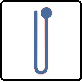
\includegraphics[angle=0,width=0.1\linewidth,keepaspectratio='true']{figures/du.png}}] BC, denotando uma marca de seleção: mostra o Menu principal
\item[\raisebox{-1em}
{
\includegraphics[angle=0,width=0.1\linewidth,keepaspectratio='true']{figures/up.png}}] C: Zoom +
\item[\raisebox{-1em}
{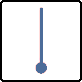
\includegraphics[angle=0,width=0.1\linewidth,keepaspectratio='true']{figures/down.png}}] B: Zoom -
\item[\raisebox{-1em}
{
\includegraphics[angle=0,width=0.1\linewidth,keepaspectratio='true']{figures/left.png}}] E: Muda a tela para cima (Normal, Aux., tela cheia)
\item[\raisebox{-1em}
{
\includegraphics[angle=0,width=0.1\linewidth,keepaspectratio='true']{figures/right.png}}] D: Muda para a tela anterior (Normal, tela cheia...)
\item[\raisebox{-1em}
{
\includegraphics[angle=0,width=0.1\linewidth,keepaspectratio='true']{figures/urdl.png}}] E, escrevendo “P”: modo Panorâmico.  Também pode ser ativado movendo-se dois dedos na tela.
\end{itemize}
\vspace{2em}

\subsection*{Mais gestos disponíveis:}
\begin{itemize}
\item[\raisebox{-1em}
{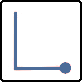
\includegraphics[angle=0,width=0.1\linewidth,keepaspectratio='true']{figures/dr.png}}] BD, escrevendo um “L”: mostra a lista de Waypoints 
\item[\raisebox{-1em}
{
\includegraphics[angle=0,width=0.1\linewidth,keepaspectratio='true']{figures/rd.png}}] DB, escrevendo um “T”: abre o gerenciador de provas
\item[\raisebox{-1em}
{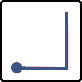
\includegraphics[angle=0,width=0.1\linewidth,keepaspectratio='true']{figures/dl.png}}] BE: mostra a lista alternativa
\item[\raisebox{-1em}
{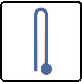
\includegraphics[angle=0,width=0.1\linewidth,keepaspectratio='true']{figures/ud.png}}]CB: ativa o Auto Zoom
\end{itemize}
\vspace{2em}

\subsection*{Gestos sofisticados:}
\begin{itemize}
\item[\raisebox{-1em}
{
\includegraphics[angle=0,width=0.1\linewidth,keepaspectratio='true']{figures/urd.png}}] CDB, escrevendo um “A”: mostra janela de análises
\item[\raisebox{-1em}
{
\includegraphics[angle=0,width=0.1\linewidth,keepaspectratio='true']{figures/ldrdl.png}}]EBDBE, escrevendo um “S”: mostra a janela de Estado. 
\end{itemize}


%%%%%%%%%%%%%%%%%%%%%%
\chapter{Navigation}\label{cha:navigation}
This chapter describes the moving map display as an aid to navigation,
and also describes some of the task and glide related overlays on the
map display.

\section{Map display elements}

\begin{maxipage}
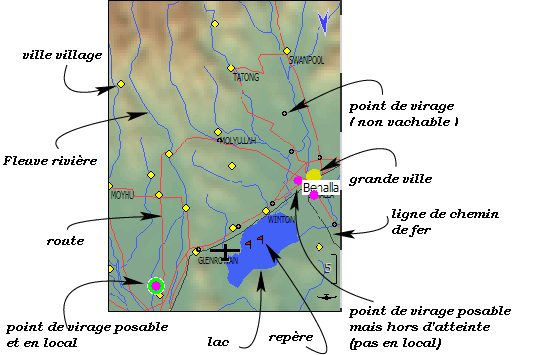
\includegraphics[angle=0,width=0.9\linewidth,keepaspectratio='true']{figures/fig-map.png}
\end{maxipage}

The moving map shows:
\begin{enumerate} 
\item Glider, wind indicator, thermal profile, final glide indicator
\item Terrain, relief and hight of the terrain
\item Topography, rivers, roads, towns
\item Waypoints, airports, landables
\item The active task, observation zones, turnpoints
\item The bearing (or route\footnote{The line to the next waypoint may be a 
  \emph{route}, as described in Section~\ref{sec:route}.}) to the next waypoint, 
  heading
\item Airspaces
\item Markers, thermals history, snail trail
\item Glide range\footnote{The glide range is also referred to as the 
  \emph{reach}, as described in Section~\ref{sec:reach}.}
\end{enumerate}
The map is drawn in a projected coordinate system (not latitude and
longitude), and the scale can be changed (zooming in and out), as well
as panned.  All navigation functions take the curvature of the Earth
into account.

\section{Glider symbol, map orientation}
The glider symbol shows the position of the glider on the map.  The
orientation of the glider indicates the estimated heading of the
glider.

The map is oriented in one of three ways: North up,
Track up, or Target up.  Configuration settings \config{orientation} can be used
to specify a different map orientation when in circling mode. This is useful to prevent
disorientation when looking at the map while circling.  Target-up when
circling makes it easy to determine which direction to exit the
thermal.

When Track or Target-up is used in circling mode, the glider symbol is
centred on the screen, even if the symbol position is configured differently.
In cruise mode the Track and the Target-up orientation allows the glider
symbol to be positioned (e.g.) 20\% from the bottom of the screen, giving a good view of the
map ahead of the glider.  This position is adjustable in the configuration
\config{gliderposition} settings.

\section{Zoom and map scale}\label{sec:zooming}

To change the scale of the map, depending on the hardware you use:
\begin{enumerate}
\item Tap/click on a blank part of the map to highlight the map if it is not
already selected.
Then use mouse wheel, or the Pocket PC up/down key to either zoom
in or out.
\item Android devices have the +/- rocker that let you change the zoom (it usually allows for adjusting the sound volume). It may be difficult to access during a flight, when the device in on a generic mount.
\item You can also gesture to change the zoom level. Gesture 
Up (see left) zooms in, Down zooms out.\gesturespec{up}
\item Or select the function from the menu.
\begin{quote}
\bmenug{Display 1}\blink\bmenug{Zoom In} and \bmenug{Zoom Out}
\end{quote}
\end{enumerate}

The map scale is displayed in the lower left corner of the moving map
display. The indicated distance is measured from the left to the right border
of the map display.
\marginpar{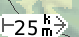
\includegraphics[angle=0,width=0.4\linewidth,keepaspectratio='true']{figures/zoom.png}}

Compaq Aero Users. If you enable the Compaq Aero Game Keys (On the
Q-menu) the centre two front buttons become the up/down keys.

\subsection*{Circling Zoom}
There is a facility to have two zoom settings; one when the glider is
in circling mode, and one in the cruise or final mode.  This is the `\emph{Circling zoom}' 
option in the \config{circlingzoom} configuration settings.  
By default, the circling zoom is set to about 2.5 km - 5.0 km, depending on the
display size. When the user zooms in or out, it affects the current
mode's zoom setting only, so when leaving the mode the previous mode's
zoom setting is used.  If `\emph{Circling Zoom}' is not enabled,
there is only a single zoom level.
This leads to different zoom levels being preserved to be managed manually, 
independent of the following Auto Zoom settings.

\subsection*{Auto Zoom}
Auto Zoom automatically zooms in when approaching a waypoint to keep
the waypoint at a reasonable screen distance. When \emph{Auto Zoom} is active,
`AUTO' appears next to the map scale.
\marginpar{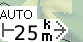
\includegraphics[angle=0,width=0.4\linewidth,keepaspectratio='true']{figures/zoomauto.png}}

To invoke Auto Zoom use the gesture \gesturespec{ud}
or menu path depicted to the left. 
Switching back to manual zoom is simply done by using the same menu path
or just zooming manually, no matter whether done via menu or gesture.
\menulabel{\bmenug{Display 1}\blink\bmenut{Zoom}{Auto}}

When a waypoint changes (automatically, via the task selector, or by
manually switching waypoints), \emph{Auto Zoom} adjusts the zoom level
automatically so that the next waypoint is visible on the map.

During circling, if a thermal has been detected, then the map is centred about
the thermal or part-way such that the glider is still visible.

\section{Panning the map}\label{sec:panning}

A pan mode allows the user to explore areas beyond the glider.  This
is particularly useful when task planning.
\begin{enumerate}
\menulabel{\bmenug{Display 1}\blink\bmenug{Pan On}}
\item Enable pan mode by button menu or by gesture.  The gesture for this is moving your fingertip up, right, down, left, supposed to form a ``P''.
\gesturespec{urdl}
\item The map can then be panned by dragging the screen or using the cursor
  keys.
\item When done, pan mode has to be disabled manually, by pressing `\emph{Pan Off}' 
  from the special sub-menu of buttons in pan mode.
\end{enumerate} 

\sketch{figures/pan.png}
When pan is active, the letters `PAN' appears next to the map scale.  While
panning the location of the focus stays in the middle of the display under the
cross hairs. 

Despite the focus under the cross-hairs the map
still offers the `\emph{What's here?}' feature just by touching any 
position on the map (presuming a touch-screen).


\section{Waypoints}\label{sec:waypoint-schemes}
Waypoints are displayed with different symbols depending on the
waypoint type; the major distinction being landable and non-landable
waypoints.

\subsection*{Landables}
The waypoint symbols are drawn as shown below. There are three icon sets for
landable waypoints. \config{waypointicons}

\begin{tabular}{c|ccc|ccc|}
Icon set 
&\begin{sideways}Landable field\end{sideways}
&\begin{sideways}Marginal\end{sideways}
&\begin{sideways}Reachable\end{sideways}
&\begin{sideways}Airfield\end{sideways}
&\begin{sideways}Marginal\end{sideways}
&\begin{sideways}Reachable\end{sideways}\\
\hline
Purple Circle &

\includegraphics[width=0.8cm]{icons/winpilot_landable.pdf} &

\includegraphics[width=0.8cm]{icons/winpilot_marginal.pdf} &

\includegraphics[width=0.8cm]{icons/winpilot_reachable.pdf} &
\colorbox{white}{
\includegraphics[width=0.8cm]{icons/winpilot_landable.pdf}} &

\includegraphics[width=0.8cm]{icons/winpilot_marginal.pdf} &

\includegraphics[width=0.8cm]{icons/winpilot_reachable.pdf} \\
\hline
B/W & 

\includegraphics[width=0.9cm]{icons/alt_landable_field.pdf} &

\includegraphics[width=0.9cm]{icons/alt_marginal_field.pdf} &

\includegraphics[width=0.9cm]{icons/alt_reachable_field.pdf} &
\colorbox[rgb]{0.94,0.94,0.94}{
\includegraphics[width=0.9cm]{icons/alt_landable_airport.pdf}} &

\includegraphics[width=0.9cm]{icons/alt_marginal_airport.pdf} &

\includegraphics[width=0.9cm]{icons/alt_reachable_airport.pdf} \\
\hline
Traffic lights & 

\includegraphics[width=0.9cm]{icons/alt2_landable_field.pdf} &

\includegraphics[width=0.9cm]{icons/alt2_marginal_field.pdf} &

\includegraphics[width=0.9cm]{icons/alt_reachable_field.pdf} &
\colorbox{white}{
\includegraphics[width=0.9cm]{icons/alt2_landable_airport.pdf}} &

\includegraphics[width=0.9cm]{icons/alt2_marginal_airport.pdf} &
\includegraphics[width=0.9cm]{icons/alt_reachable_airport.pdf} \\
\hline
\end{tabular}

The \emph{marginal} icons are drawn for those waypoints which are principally in the 
reach, but it is not possible to approach them directly. E.g.\ a mountain prohibits a direct approach.
  
Waypoints are optionally labelled according to one of several
abbreviation schemes \config{labels} and visibility.

On top of this landable waypoints can be displayed in more detail. If
`\emph{Detailed landables}' is switched on you get additional information
encoded in the appearance of it's icon. 
\begin{enumerate}
\item  Landable fields get a square-shaped icon despite what is shown in the table.
  The square is drawn like a diamond standing on one corner. Airfields stay with the 
  circle shape, so that they become easy to distinguish.
\item  All icon sets, including the `Purple Circle' icon set, get the 
  runway turned into their actual direction. The runway direction has to be available in 
  the waypoint data. E.g.\ the SeeYou waypoint file format (\verb|.cup|) does
  include this information.  
\end{enumerate}

\subsection*{Landables in Reach}
Next to landables an estimated arrival height
\emph{above the arrival safety height of reachable landable} points is
displayed next to the waypoint. This feature is one of the most powerful out 
of XCSoar's capabilities. The arrival height is calculated highly 
configurable by XCSoar's \emph{glide computer} with parameters taken into 
account being glider performance (polar), MacCready setting, wind, terrain 
clearance, and --- obviously --- safety heights' values.
With all of it being 
configurable, there is enough room for failure, so please:
Unless you will have fully understood the glide computer's concepts, you 
\warning
better stay with XCSoar's pre-configuration (and in no way judge readings as 
heavenly approved).
It is up to the pilot to always interpret readings and watch values trending 
over time.

However, having set up the glide computer following
Chapter~\ref{cha:glide} the \emph{display} of estimated reach heights, drawn beside 
landables in reach may take into account terrain or not or display both.
\config{arrivalheight}

Another option is to display the required glide ratio next to a landable in 
reach. This calculation is simply derived by the glider's actual distance to 
landables divided by the height difference between actual altitude and 
landable's altitude.  Again, the safety height is added to the landable's 
height, but nothing else taken into account: no wind, no polar, no MacCready 
settings, just geometry. The concept of required glide ratios is a widely 
discussed concept, said as to be a very robust one.

\tip Keep in mind a strong relationship of displays of \emph{reach} and 
settings in the glide computer.

\subsection*{Non-Landables}
As far as your waypoint file contains information on the nature of the 
non-landable waypoints, the map will then display specific icons accordingly. 
Figure~\ref{fig:nonlandables} contains a collection of the currently supported map icons.

\begin{figure}[htbp]
\centering
\vspace{2.5cm}
\begin{tabular}{ccccccccc}
\begin{rotate}{60}Simple waypoint\end{rotate} &
\begin{rotate}{60}Mountain top\end{rotate} &
\begin{rotate}{60}Obstacle\end{rotate} &
\begin{rotate}{60}Pass\end{rotate} &
\begin{rotate}{60}Power plant\end{rotate} &
\begin{rotate}{60}Tower or building\end{rotate} &
\begin{rotate}{60}Tunnel\end{rotate} &
\begin{rotate}{60}Weather station\end{rotate} &
\begin{rotate}{60}Bridge\end{rotate}\\

\includegraphics[width=0.5cm]{icons/map_turnpoint.pdf} &
\includegraphics[width=0.8cm]{icons/map_mountain_top.pdf} &
\includegraphics[width=0.7cm]{icons/map_obstacle.pdf} &
\includegraphics[width=0.7cm]{icons/map_pass.pdf} &
\includegraphics[width=0.8cm]{icons/map_power_plant.pdf} &
\includegraphics[width=0.7cm]{icons/map_tower.pdf} &
\includegraphics[width=0.6cm]{icons/map_tunnel.pdf} &
\includegraphics[width=0.6cm]{icons/map_weather_station.pdf} &
\includegraphics[width=0.8cm]{icons/map_bridge.pdf}
\end{tabular}
\caption{non-landables}\label{fig:nonlandables}
\end{figure}

\section{Active task}

The active task course is drawn on the map as a blue (dashed) line.

Assigned area tasks also show the turn point sectors or areas as a yellow shaded
region.  Circles are always drawn around start and finish points, lines are
only drawn if the start/finish points are of line type.  
Task observation sectors are drawn as circle segments.

At all times a thick black line is drawn from the glider to the next
waypoint in the task.  This line may be the direct path to the waypoint,
or may be a \emph{route} path clearing terrain and airspace obstacles, described in
further detail in Section~\ref{sec:route}.

\begin{center}
\begin{tabular}{c c c}
\emph{Start/finish} & \emph{Sector} & \emph{Cylinder} \\
\includegraphics[angle=0,width=0.3\linewidth,keepaspectratio='true']{figures/cut-startfinish.png} &
\includegraphics[angle=0,width=0.3\linewidth,keepaspectratio='true']{figures/cut-sector.png} &
\includegraphics[angle=0,width=0.3\linewidth,keepaspectratio='true']{figures/cut-barrel.png}
\end{tabular}
\end{center}


\section{Terrain and Topography}\label{sec:terrain_topo}

The following topographical features are drawn on the map:
\begin{itemize}
\item Major roads, shown as red lines
\item Rivers, shown as blue lines
\item Large water bodies (lakes), shown as blue areas
\item Large cities, shown as yellow areas
\item Small population areas, shown as yellow diamonds
\end{itemize}
Cities and small population areas are labeled in italics.

Terrain is coloured according to elevation, and optionally shaded by sun, or 
wind direction.  Invalid terrain, or terrain below
sea level is coloured blue.

\menulabel{\bmenug{Display 2}\blink\bmenut{Terrain}{On/Off}}
\menulabel{\vspace{1cm}\bmenug{Display 2}\blink\bmenut{Topo.}{On/Off}}

Terrain is shaded to improve visibility.  The default shading
is set up so that the virtual lighting position is the wind bearing,
thus brighter areas are on the upwind side of hills and dark areas in
the lee of the hill.  
Support for a sun ephemeris is also implemented. If the slope shading is set 
to `Sun', the brightness of a slope follows the day time in a very natural way.
The amount of shading and overall terrain brightness is configurable. \config{shading}

Both terrain and topography display can be switched on or off from the
menu.

\begin{center}
\begin{tabular}{c c}
Topography & Terrain \\
\includegraphics[angle=0,width=0.4\linewidth,keepaspectratio='true']{figures/cut-topo.png} &
\includegraphics[angle=0,width=0.4\linewidth,keepaspectratio='true']{figures/cut-terrain.png}
\end{tabular}
\end{center}

If the terrain data is not available (or terrain display is turned
off), the background colour of the map window is white.  All terrain
below mean sea level is coloured blue.  If you are flying outside the
terrain region, the background colour will be white.

\subsection*{Map labels}\label{sec:maplabels}

The screen can be de-cluttered, turning off the display of all waypoint labels by toggling the `\emph{Labels}' menu.
\menulabel{\bmenug{Display 2}\blink\bmenut{Labels}{None}}

Other options for display decluttering include:

\jindent{\bmenuth{Labels}{Task \&}{Airfields}}{ Shows labels for the waypoints in 
  the active task and any airfields (based on the waypoint attributes in 
  the waypoints file).  Other waypoints are shown but not labeled. }
\jindent{\bmenut{Labels}{All}}{ Shows labels for all waypoints. }
\jindent{\bmenuth{Labels}{Task \&}{Landables}}{  Shows labels for the waypoints in 
  the active task and any landable fields (based on the waypoint attributes in 
  the waypoints file).  Other waypoints are shown but not labeled. }
\jindent{\bmenut{Labels}{Task}}{ Shows labels only for waypoints in the active task}

Note that in all cases, the label format is configurable in the 
`\emph{Waypoint Display}' configuration menu.  \config{labels}


\section{Trail}\label{sec:trail}

An optional `snail trail' is drawn on the map showing the glider's
path history.  The colour and thickness of the trail depends on the altitude or
on the variometer value. 

\begin{center}
\includegraphics[angle=0,width=0.5\linewidth,keepaspectratio='true']{figures/snail.pdf}
\end{center}

If Vega or an intelligent variometer is connected with Netto output,
the Netto vario value is used; hence the colours and thickness of the
trail indicates the air-mass vertical movement rather than the glider's
vertical movement.

\config{snailtrail}
The snail trail display can be toggled between \emph{Off}, a \emph{Short} trail
(about ten minutes), a \emph{Long} trail (about one hour) or a \emph{Full} trail
which displays the entire flight.  This can be performed permanently
through the configuration settings or temporarily by the
menu.
\menulabel{\bmenug{Display 2}\blink\bmenut{Trail}{Full}}

Note that for all of these modes, the snail trail is short in
circling mode in order to reduce screen clutter.

In order to assist centring thermals in the presence of wind, the
snail trail can be artificially drifted with the wind as it is
displayed (this is drift compensation).  In this way, the snail trail
is referenced to the prevailing wind rather than referenced to the
ground.  Since thermals drift with the wind also, the drifted trails
give a better indication of where the glider has been relative to the
thermals.

An example of this is illustrated below.  Note that when trail drift
compensation is active (right picture), the glider appears to be
circling in a column rather than an elongated spiral (left picture).

\begin{center}
\includegraphics[angle=0,width=0.6\linewidth,keepaspectratio='true']{figures/traildrift.png}
\end{center}

\config{traildrift}
Enabling trail drift compensation is performed through the
configuration settings.  The compensation is only performed
whilst in circling mode; the display of the trail in cruise mode is unaffected.
This can also be performed from the wind settings dialogue.
\menulabel{\bmenug{Config 1}\blink\bmenus{Wind}}

The trail drift display is useful also to show more clearly when thermals
are cranked due to wind shear.

The trail width can optionally be scaled according to the variometer display\config{trailscaled}.


\section{Markers}\label{sec:markers}

Markers are shown as small flags (a) on the map.  The markers can be dropped
manually, by pressing a button, or automatically.  An example use of
automatic markers is to drop markers when entering circling mode, as a
simple way of showing all thermals encountered.

\menulabel{\bmenug{Nav 2}\blink\bmenut{Mark}{Drop}}
Markers are not preserved after XCSoar is exited, however the location
of all marks are appended to the file \verb|xcsoar-marks.txt|.

\section{Pilot Event}\label{sec:pilotevent}

A Pilot Event (PEV) system allows pilots to mark particular times during a
flight, such when inside a Turn Point Observation Zone (TP OZ). Also, when
configured, it allows to initiate a special \emph{Pilot Event} task start
protocol\footnote{PEV start procedure may be used in competitions to reduce
mass starts, gaggles and following.}.

\menulabel{\bmenug{Nav 2}\blink\bmenut{Pilot}{Event}}

When pressed, the task start window will be automatically set according to
configuration defined in Task Rules (See \ref{sec:task-type-racing}): start
window will open after \emph{PEV start wait time} \config{taskrules} minutes
and will be open for \emph{PEV start window} minutes.  Also, \emph
{Pilot Event} will be announced to connected devices, allowing loggers to
register it without pilot pressing the physical button on the logger device
itself. This might be useful when logger is located outside of pilot reach
(e.g. behind the panel).

In order to start a task when \emph{Pilot Event Start} is used, press the \emph
{Pilot Event} button, wait for \emph{PEV start wait time} and then cross the
start line within \emph{PEV start window} minutes.

\tip It may be useful to have \emph{Start open} and/or \emph{Start reach}
 infoboxes visible to effectively use the \emph{PEV Start} procedure.


\section{Thermals}

While climbing in thermals, a marker is automatically generated showing the
thermal location on screen.    The positions of the last 20 thermals are
stored until the end of the flight.
\sketch{figures/thermalhistory.png}
This thermal history is accessible through the map
element functions in the same way as markers or waypoints.


\section{Glide range line}\label{sec:reach}

A reachable glide `footprint' is displayed on the map display as a
black and white dashed line, indicating where the glider would descend
through the terrain clearance height.  The reach shows clearance
tracks extending in all directions, optionally including paths around
terrain obstructions.  This feature is useful in assessing range with
respect to topography when searching low for lift, and when flying in
mountainous areas.

Reach calculations may be configured \config{turningreach} to two levels of detail:
\begin{description}
\item[Straight line] If turning reach is disabled, then the reach shows the
 furthest distance the glider can fly in final glide in all directions without
 turning.  This reach appears as a closed ring around the glider.

\begin{center}
\includegraphics[angle=0,width=0.8\linewidth,keepaspectratio='true']{figures/reach1.png}
% CUTOUT SHOWING GLIDE RANGE FOOTPRINT.  NO TOPOGRAPHY, FULLSCREEN, NO TASK. TURNING=FALSE
\end{center}

\item[Turning] If turning reach is enabled, then the reach shows the
  greatest area the glider can reach in all directions, even allowing
  turns around obstructions.\footnote{The maximum number of turns is
    set to three, and no turns may be greater than 90 degrees.}  The
  reach area appears as a closed ring around the glider but may also
  include holes indicating mountain peaks that the glider cannot reach
  without further climb.

\begin{center}
\includegraphics[angle=0,width=0.8\linewidth,keepaspectratio='true']{figures/reach2.png}
% CUTOUT SHOWING GLIDE RANGE FOOTPRINT.  NO TOPOGRAPHY, FULLSCREEN, NO TASK. TURNING=TRUE
\end{center}

\end{description}

The display can be configured to additionally blur the unreachable area
outside the glide range. \config{gliderange}
The final glide path is checked for whether the glider clears terrain along
the path by the terrain clearance height (see Section~\ref{sec:safety-heights}).
If clearance is not attained, a red
cross appears on the map at the point where the violation occurs. If a target is
defined the calculation is done along the straight path to the target. If no 
target is defined the calculation is done along the current heading.

If reach is enabled, then the reachability of landable waypoints is used
by the abort task mode, alternate landable option lists and display of
landable waypoints on the map.

Note that task calculations are otherwise unaffected by reach
calculations --- for example, altitudes required as shown in the final
glide bar or task data as displayed in infoboxes do not take reach into account.

Furthermore, the reach calculations are used for footprint, landable
waypoint arrival heights, abort mode and the alternates dialogue.  The glider
performance and MacCready setting used in these calculations are configurable\config{reachpolar}:
\begin{description}
\item[Task] The MC value is that used in the task.
\item[Safety MC] A configurable, typically low MC value is set by the user to set
  performance near, but slightly degraded, to best glide performance. The amount of safety 
  in the reach calculation is then the gap between best glide performance and the glide
  performance following the safety MC speed to fly. 
\end{description}

\section{Status tabs `\emph{Flight}' and `\emph{Time}'}\label{sec:flight-status}

The status dialogue is a multi-tabular dialogue giving overview information on the 
flight, system, task, rules and times.
These are information, and hence cannot be modified by the user.
It is accessed via the gesture ``S'', or with the button menu.
\gesture{Left - Down - Right - Down - Left}
\begin{quote}
\bmenug{Info 2}\blink\bmenug{Status}
\end{quote}

\subsection*{Flight}
Select the tabular page `\emph{Flight}'. 
The flight status dialogue shows the status of the aircraft's locality.
It shows the location of the aircraft, the
maximum height gain, and nearest waypoint it's bearing and distance.
\sketch{figures/status-flight.png}

You may find this function useful when you need to report your
location to others.

\subsection*{Times}\label{sec:time-status}
Select the tabular page `\emph{Times}'. 
It shows the local time, UTC time and date, flight duration, takeoff and landing time, and
the local sunrise and sunset times.

Note that the values in the Status dialogue 
are static once the particular dialogue page is displayed. 
\sketch{figures/status-times.png}
That is, position, times, etc.\ do not update while the page is displayed.
To see the updated values, it is necessary to select a different tabular, 
then return to the previous dialogue to see the new values.


\section{Route}\label{sec:route}

XCSoar can plan paths around terrain and airspace obstacles in three
dimensions from the aircraft to the destination.  Such a path is known
as a route.  The height of the destination is the arrival height for
final waypoints, or may be higher for intermediate waypoints, as
dictated by the task system as required to complete the task.  Route
planning functions in normal ordered task mode, abort mode and goto
mode.

\begin{center}
\includegraphics[angle=0,width=0.8\linewidth,keepaspectratio='true']{figures/route3.png}
\end{center}

Routes take into account the glider polar performance and are
calculated to be optimal in the sense of minimum time.  By default,
route calculation is disabled, and can be enabled for terrain only or
terrain and airspace avoidance. \config{routemode}

Terrain is avoided vertically by the terrain safety height,\config{safetyterrain}
with no additional lateral clearance imposed.
Valid routes may result in the aircraft arriving at the destination
higher than the minimum height --- such as can occur when the
destination is just beyond a steep mountain.

Airspace is avoided horizontally by a buffer of approximately 250 m,
with no additional vertical clearance imposed.  Valid routes may fly
below or above airspace.

If MacCready is positive, then climbs are optionally allowed
 in the computed routes.  The top of the climb
may be limited to 500 m above the higher of the start and destination
ceiling, or increased to the ceiling defined by the thermal ceiling.
\config{routeceiling}  Climbs above the higher of the start and
destination altitude are penalised by a slower climb rate than the
actual MacCready value.

Some approximations and limitations of the route planning system are as follows:
\begin{itemize}
\item Where climbs are necessary (and permitted) to reach the destination,
the climbs are assumed to occur at the start of the route.
\item Climb-cruise segments are assumed to occur at constant altitude,
equivalent to many small climbs distributed along the path.
\item Individual turns between path segments greater than 90 degrees
  are not permitted.
\item Failures of the solver result in the route reverting to direct flight
from the aircraft location to the destination.
\end{itemize}


%%%%%%%%%%%%%%%%%%%%%%
\setcounter{chapter}{4}
\chapter{Überlandflug Aufgaben - Navigieren mit\textsf{XCSoar}}\label{cha:tasks}
\index{Aufgabe}\index{Tasks}

\textsf{XCSoar} bietet ein ausgefeiltes, komplettes Aufgabenmanagementsystem, mit dem Aufgaben vor und während des Fluges erstellt, editiert und auch gelöscht werden können.

Die Wendepunkte können vollautomatisch angeflogen und umgestellt werden, wobei die Kartendarstellung automatisch hinein- bzw. herausgezoomt werden kann. Ein rein manuelles  Anwählen und Umschalten ist aber ebenso möglich.

Dieses Kapitel beschreibt weiterhin die Benutzung von \textsf{IGC} Loggern mit\textsf{XCSoar}

Intern werden drei Aufgabentypen (modi)  unterschieden
\begin{description}
\item[\p{Deklarierte Aufgabe}] Dies ist der eigentliche Überlandflug-Modus, bei dem ein Startpunkt, ein
    Zielpunkt und mehrere Wendepunkte deklariert sein können. Die Wendepunkte müssen in der
    angegeben Reihenfolge angeflogen werden. (Leistungsflug)\index{Task!Leistungsflug}
\item[\p{''Ziele auf''-- Aufgabe}] Ein Flug auf exakt ein einziges Ziel zu. (Irgendein Flug)\index{Task!Zielflug}
\item[\p{Abort - Aufgabe}] Hier wird "frei" durch die Gegend geflogen, ohne einen Wegpunkt als  Ziel
    deklariert zu haben. (Lustflug)\index{Task!Lustflug}
\end{description}

 Beachte, daß im ''Ziele auf''- und im Abort - Modus  die  evtl.\ abgebrochene Aufgabe \textsl{jederzeit} wieder \tip aufgenommen werden kann, dies unter Beibehaltung sämtlicher bisher aufgenommenen Berechnungen und Statistiken.

\section{''Ziele auf''-- Aufgabe}\index{Aufgabe!''Ziele auf'-'-Typ}\index{Task!''Ziele auf''}

''Ziele auf''--Aufgaben'' können erstellt werden, indem man einen Wegpunkt auf der Karte markiert und anschließend auf dem ''Kartenelemente an diesem Ort'' oder dem Wegpunkt-Detailfenster mit "Ziele auf" bestätigt.  Alternativ kann auch über den "Alternative" Dialog zu einem Wegpunkt gelangt werden, welcher anschließend mit ''Ziele auf'' festgelegt wird.

Während des ''Ziele auf''--Modus \menulabel{\bmenut{Nav}{2/2}\blink\bmenut{Aufgabe}{fortsetzen}} kann eine vorher abgebrochene Aufgabe immer wie links fortgesetzt werden.

\subsection{Automatik ''Ziele auf''}\index{Automatik--''Ziele auf''}\index{Heimatflugplatz!Automatik}

Wenn keine deklarierte Aufgabe geladen ist, dann wird nach dem Start unverzüglich in den ''Ziele auf''--Modus geschaltet. Hierbei wird der Startplatz oder aber (falls es z.B. eine Wiese war, von der man mit einer Wilga im F-Schlepp gestartet ist), der nächstgelegene landbare Flugplatz automatisch als Ziel in den Rechner eingefügt.

Egal, ob eine Aufgabe deklariert wurde, oder nicht, es wird grundsätzlich ein Startpunkt erfaßt, welcher für spätere Benutzung während des Fluges in der Wegpunktliste erscheint und ganz normal  verwendet werden kann. 
Dieser Punkt ist auf der Karte als ''take-off' gekennzeichnet' \todonum{wird der auch gespeichert? wo ?}

\section{Aufgaben erstellen und bearbeiten}\index{Aufgabe!Erstellen}\index{Aufgabe!Bearbeiten}

Aufgaben können auf unterschiedliche Weise erstellt und editiert  werden. Manche Methoden eigentlich mehr für die Bearbeitung und Erstellung vor dem Flug,  andere erlauben es eine Aufgabe während des Fluges zu ergänzen bzw. zu verändern.

Aufgaben können in Dateien (Files) gespeichert werden um später geladen zu werden oder aber um zwischen verschiedenen Geräten hin und her kopiert zu werden. Alle\textsf{XCSoar} Plattformen sind Dateiformatskompatibel d.h.\  jede Aufgabe kann auf jedem\textsf{XCSoar} erstellt, geflogen und gespeichert werden. (\textsf{PC, Android, MAC)}).

\tip Es ist möglich (und sinnvoll) eine Standard-Aufgabe zu erstellen und zu speichern und diese  Aufgabe beim jedem Start von\textsf{XCSoar} automatisch laden zu lassen.

Eine Anwendung dieser Standardaufgabe ist zum Beispiel, einen Wegpunkt  als Heimatflughafen zu deklarieren. d.h.,  der Heimatflugplatz ist anschließend grundsätzlich automatisch als Ziel eingestellt, wenn man einfach nur durch die Gegend fliegen will.

Die Möglichkeiten, Aufgaben zu erstellen sind wie folgt:
\begin{itemize}
\item Benutzen des Aufgabeneditor-Dialogs
\item Auswählen eines Wegpunktes von der Karte und hinzufügen zur Aufgabe über den Wegpunkt Detail-Dialog.
\item Laden einer Aufgabe aus einer Datei.
\end{itemize}

\tip Aufgaben in einer Datei zu sichern und anschließend wieder zu laden ist sehr sinnvoll,  will man zum Beispiel mit mehreren Piloten eine gleiche Aufgabe fliegen oder aber im Wettbewerb ist, wo im  allgemein die Aufgaben vorher deklariert und eingegeben werden.

Entscheidend hierbei ist, daß lediglich eine Person die Aufgabe eingeben muß und diese anschließend  per copy \& paste,  Bluetooth oder Kabel kopiert werden kann.

\textsf{XCSoar} sichert die aktuelle Aufgabe beim Herunterfahren und lädt die gleiche Aufgabe wieder beim Neustart.  Die Wegpunkte einer Aufgabe sind sogar gesichert, wenn die Wegpunktdatei gewechselt wird. d.h., wenn eine Aufgabe gespeichert wird, anschließend das Wegpunktfile gewechselt wird, die gleiche Aufgabe wieder geladen  wird, wenn die Wegpunkte, welche in der Wegpunktdatei  fehlen automatisch durch die Wegpunkte aus der Aufgabe ergänzt.

\section{Wegpunkt Info und Details }\index{Wegpunkte!Details}

Der Wegpunkt-Info-Dialog beschreibt die Details der Wegpunkte  und bietet Navigations-Optionen wie zum Beispiel \textsf{Ziele auf}, \textsf{Einfügen} oder \textsf{Anhängen} an einer Aufgabe. Weiterhin kann über diesen Dialog ein Wegpunkt als Heimatflughafen eingegeben werden.

Die Anwahl  kann über mehrere Wege erfolgen:
\begin{itemize}\itemsep=1em
\item
Über die Karte, wenn der Wegpunkt sichtbar ist: \\
Ein \textit{einfacher} Klick öffnet das "Kartenelemente an diesem Ort''-Fenster.

Anschließend auf \button{Details} drücken.
%
%
\item
Über das Menü
\begin{quote}
\button{Nav}\blink\button{Alternativen}, Auswahl des Punktes und \button{Details}
\end{quote}
%
%
\item Über den Aufgabeneditor: \index{Wegpunkte!Anwahl}
\begin{quote}
\button{Nav}\blink\button{Aufgabe}\blink\button{Wendepunkte}\blink\button{Wendepunkt  hinzufügen}, Auswahl des Punktes und \button{Details} oder Doppelklick 
\end{quote}
%
%
\item%[\Large{$\bullet$}]
Vom Wegpunkt-Auswahlmenü \button{Nav}\blink\button{Wegpunkt Liste} und \button{Auswählen}
(Hier kann mittels eines einiger Filters besonders schnell und elegant jeder beliebige Wegpunkt auf schnellstmögliche Weise ausgewählt werden. Sehr effektiv, wenn man nicht nur den nächst möglichen Wegpunkt anwählen will.)
%
%
\end{itemize}

Der Wegpunktdetail-Dialog enthält zwei maßgebliche Seiten, welche über \button{$>$} und  \button{$<$} weiterschaltbar sind. Je nach dem, ob noch weitere Informationen zum Wegpunkt vorliegen, erscheinen Seiten mit weitere Details hierzu.

Auf dieser Seite werden Details zum Wegpunkt wie z.B.\ Funkfrequenz, Länge der Bahn, Höhe, Art der Bahn, Namen, Peilung (Bearing), Sonnenuntergang Entfernung zum Wegpunkt. etc.\ angegeben.

Zusätzlich befindet sich ein Button \button{Fliege Zu} um direkt zu diesem Punkt zu navigieren.  Dieser Button brichtt die aktuelle Aufgabe, sofern vorhanden, ab.

\sketch{{figures/dialog-waypointdetails0.png}}
Wie bereits oben erwähnt, zeigt der Wegpunkt-Info-Dialog drei Höhendifferenz-Angaben zum Erreichen des Wegpunktes, welche hier unten beschrieben werden:

\begin{description}
\item[\p{Ortskoordinaten}] Die Koordinaten des Punktes in Grad, Minuten und Sekunden
\item[\p{Höhe}] Die Höhe (MSL) des Punktes
\item[\p{Tageslichtzeiten}] Sonnenauf- und Untergang
\item[\p{Peilung und Distanz}] Richtung und Entfernung zum Punkt
\item[\p{H Diff MC 0}] Benötigte Höhe bei MacCready Null
\item[\p{H Diff MC sicher}] Benötigte Höhe bei Sicherheits MacCready (s. Kap~\ref{sec:safety-factor})
\item[\p{H Diff MC aktuell}] Benötigte Höhe bei  aktuell eingestellten MacCready Wert
\end{description}

Über die Buttons \button{$<$} und \button{$>$} in der linken unteren Ecke des Fensters können weitere Seiten mit Informationen über den aktuellen Wegpunkt angewählt werden. Weiterhin wird damit ein Menü geöffnet, auf dem z.B. dieser Wegpunkt als Ziel, Heimat oder Aufgabenwegpunkt eingefügt werden kann.


\subsection*{Flugplatz Informationen}
Diese Seite kann -sofern Daten zum Flugplatz vorhanden- etliche Hinweise und Details zu Flugplätzen enthalten. \sketch{figures/dialog-waypointdetails1.png}
Insbesondere sind hier enthalten Details zur Landebahn, Landebahnrichtung, Höhe, Frequenz usw.


\subsection*{Satelliten Photo}
Sofern vorhanden, kann hier z.B.\ ein Foto des Flugplatzes eingefügt und angezeigt werden. 
Näheres hierzu siehe Kap.~\ref{sec:airfield-details} 


\section{Wegpunkt-Auswahl-Dialog}\label{sec:waypoint-selector-dialog}
Der Wegpunkt-Auswahl-Dialog ist \textsl{der} Dialog, von dem aus Wendepunkte die in einer Datenbank (Datei) \menulabel{\bmenut{Nav}{1/2}\blink\bmenut{Wegpunkt}{Liste}}enthalten sind, ausgewählt werden kann.

Die Wegpunktlisten-Auswahlseite bietet einen Satz an von vier Filtern, um die Auswahl der entsprechenden \gesture{Runter -Rechts} Wegpunkte schneller und effizienter zu machen. Diese Filter können einzeln, gar nicht oder alle zusammen benutzt werden, umso die Auswahl eines Wegpunkt  einzugrenzen.

Folgende Wegpunktfilter sind vorhanden:

\begin{description}
\item[\p{Name}] Dieser Filter bietet eine sehr schnelle Möglichkeit, Wegpunkte anhand des Namens herauszufiltern.
\item[\p{Distanz}] Über diesen Filter werden die Wegpunkte nach der Entfernung angeordnet. Die nächstgelegene 
Mittelpunkte werden an die Spitze der Liste gesetzt.
\item[\p{Typ}] Über diesen Filter werden die Wegpunkte anhand ihrer Eigenschaft (Flugplatz, Landefeld, Startpunkt, oft benutzt, enthalten im Wegpunktdatei 2), usw. ausgewählt.
\item[\p{Richtung}] Hiermit werden Wegpunkt ausgewählt, welche in der entsprechenden gewünschten Richtung liegen. Ein besonderer Filter hierbei ist der Heading-Filter (\textsf{HDG(0$^\circ$)}) welcher nur Wegpunkte anzeigt, die sich in einem Winkel von $\pm 30\circ$ zur Flugrichtung befinden.
\end{description}

Wenn die Filterung nach Namen und gilt gewählt wird, ist die Ergebnisliste nach dem Namen geordnet. Wenn (auch zusätzlich) die Wegpunkte nach Entfernung oder Richtung gefiltert werden, dann erfolgt die Sortierung der Wegpunkte grundsätzlich als erstes nach der Entfernung.
D.h., der als nächste gefundene Wegpunkt wird immer an die Spitze der Liste gesetzt.

\sketch{figures/dialog-waypointselect.png}
Diese Ergebnisliste kann durchgescrollt werden, wenn Sie Einträge mehr als auf einer Seite dargestellt werden können. Um zu scrollen, einfach mit dem Finger auf dem TouchScreen hoch und runter, alternativ mit der Maus ans Ende oder Spitze der Liste fahren.

Je nachdem aus welcher Situation die Wegpunktauswahl aufgerufen wurde, kann das Verhalten unterschiedlich sein. Normalerweise bringt die Anwahl eines Wegpunktes aus der Liste  direkt das Wegpunkt-Detail-Fenster.

\section{Aufgabenverwaltung }\label{sec:task-manager-dialog}
Die Aufgabenverwaltung wird benutzt, um Aufgaben zu erstellen, zu löschen, zu \menulabel{ \bmenut{Nav}{1/2}\blink \bmenus{Aufgabe}}speichern und zu deklarieren. 
Sie ist in der Zwischenzeit massiv überarbeitet und komplett neu gestaltet worden.

Gegenüber früheren Versionen von \textsf{XCSoar} befindet sich so gut wie nichts mehr an der gewohnten und üblichen Stelle. 

Das Arbeiten mit der neuen Version hat sich jedoch erheblich vereinfacht und ist deutlich komfortabler, übersichtlicher und schneller geworden.

Die Startseite der Aufgabenverwaltung ist der Rechner. Hier werden diverse berechnete Werte angezeigt, die \menulabel{\includegraphics[keepaspectratio,width=0.4\textwidth]{figures/dialog-taskcalculator.png}}aktuelle Aufgabe betreffen und im Detail weiter unten beschrieben werden.

Weiterhin stehen folgende Buttons zur Verfügung:

  \p{Rechner}, \p{Wendepunkte}, \p{Verwalten}, und \p{Regeln}, sowie selbstverständlich \p{Schließen}, um die Aufgabenverwaltung zu schließen.

\subsection*{Wendepunkte}
Der Button  \button{Wendepunkte} zeigt eine Liste der aktuell in der jeweiligen Aufgabe bestimmten Wegpunkt. Wenn kein Wegpunkt In der aktuellen Aufgabe gelistet ist, gibt es nur eine einzige Option, und zwar die, einen Wegpunkt hinzuzufügen: "Wegpunkt hinzufügen"

Durch Drücken auf die graue "Wendepunkt hinzufügen" Schaltfläche wird die Wegpunkt Auswahl gestartet (siehe
oben).  Ein hier ausgewählter Wegpunkt erscheint anschließend in der Aufgabe.

\subsection*{Verwalten}
Durch Drücken auf den Button \button{Verwalten} wird die Verwaltung der Aufgaben geöffnet, hierbei erscheinen vier große Schaltflächen:

\begin{itemize}
\item \button{Neue Aufgabe} Löscht die aktuelle Aufgabe und setzt die Regeln auf die Standardwerte.
\item \button{Anmelden} Wenn ein externer Bürger angeschlossen ist, wird hiermit die aktive Aufgabe an den Logger übertragen und somit deklariert.
\item \button{Durchsuchen} Zeigt eine Liste aller gespeicherten Aufgaben, und erlaubt es, Aufgaben zu laden. Beachte, daß diese Option die aktuelle Aufgabe löscht.
\item \button{Speichern} Sichert die aktuelle Aufgabe. Nachdem die Schaltfläche berührt wurde, wird der Not aufgefordert, einen Namen zu vergeben, unter dem die Aufgabe gespeichert wird und wieder geladen werden kann.
\end{itemize}

\subsection*{Regeln}\index{Regeln}
Die Werte, die bei Anklicken des Buttons \button{Regeln} erscheinen, hängen vom Typ der Aufgabe ab, die vorher erstellt wurde.

Durch Anklicken der jeweiligen weiß hinterlegten Werte wird ein Untermenü geöffnet, auf dem diese Werte entsprechend geändert werden können. Die diversen Aufgabentypen werden in einem Abschnitt weiter unten besprochen.

Ein erneutes Drücken des Buttons  \button{Regeln} öffnet eine Kartenansicht der aktuellen Aufgabe. Erneutes Anklicken des Buttons führt wieder zu den einzelnen werden.

\subsection*{Aufgabentypen}\index{Aufgabentypen}

\textsf{XCSoar} unterstützt derzeit folgenden verschiedenen Aufgabentypen:
Racing, AAT und FAI Abzeichen/Rekorde.

Eine Kurzbeschreibung der diversen Aufgabentypen erfolgt erfolgt unten. In diesem Handbuch sollen aber nicht die kompletten FAI Regeln wiederholt werden. Für eine ausführliche Beschreibung der jeweiligen Aufgabentypen kann  auf der Homepage der FAI nachgeschaut werden: \url{http://www.fai.org}.

\begin{description}
\item[\p{Racing}] Eine  "racing" Aufgabe besteht aus einem Startpunkt, mehreren Wendepunkt,  und einem Zielpunkt, welche in vorgeschriebener Reihenfolge und so werden müssen. (Wenn hier unter "Regeln" FAI Start/Zielregeln auf "Ein" geklickt ist dann sind keiner weiteren Optionen verfügbar FAI-Regeln sind fix).\index{Regeln!Racing}
        \begin{itemize}
            \item max. Abfluggeschwindgkeit:     Hier wird die maximale Abfluggeschwindigkeit, die vom Veranstalter vorgegeben wird, eingestellt. Wenn die Abfluggeschwindigkeit nicht limitiert ist, sollte der Wert "0"  eingestellt werden.
            \item Maximale Abflughöhe: Hier wird die maximale Abflughöhe eingetragen, die der Veranstalter vorgibt.   Wenn die Abflughöhe nicht limitiert ist, sollte hier "0" eingetragen werden.
            \item Abflughöhe bezogen auf: Hier wird eingetragen, ob die Abflughöhe auf den Startpunkt (AGL) oder aber auf  Meereshöhe (MSL) bezogen ist.
            \item Minimale Ankunftshöhe:  Dies ist die vom Veranstalter vorgegebene minimale Ankunftshöhe. Ist keine vorgegeben, so sollte hier "0"  stehen.
            \item Zielhöhenref.:  Hier wird eingetragen, ob die Ankunftshöhe auf den  Startpunkt (AGL) oder aber auf  Meereshöhe (MSL) bezogen ist.
            \item FAI Start/Zielregeln: Wenn hier ein angeklickt wurde,  dann  gelten die FAI-Regeln. D.h., es gibt keine maximale Starthöhe und keine maximale Abfluggeschwindigkeit. Die Zielhöhenreferenz ist bezogen auf den Startpunkt (AGL) und die minimale Ankunftshöhe beträgt 1000m oberhalb der Starthöhe. 
    \end{itemize}
\item[\p{AAT}]
 Dieser Aufgabentyp beschreibt eine  Aufgabe, bei der um verschiedene Wendepunkte herum gewisse Flächen (Kreise, Segmente, ö.ä) gezeichnet sind, in denen jeweils mindestens ein Punkt gelegt werden muß werden muss.
 Es wird eine \textsl{mindestens} zu fliegende Zeit vorgegeben.
    \begin{itemize}\index{Regeln!AAT}
            \item AAT min. Zeit:  Diese Zeit muß mindestens geflogen werden, um eine Wertung ohne Punktabzug zu bekommen. Eine Ankunft am Zielpunkt, bevor die Mindestzeit abgelaufen ist, wird in der Regel mit Strafpunkten bewertet und ist in aller Regel mit einem schlechteren Schnitt versehen.
        	\item Max. Abfluggeschwindigkeit: Identisch wie bei der Racing-Aufgabe
        	\item Maximale Abflughöhe: Identisch wie bei der Racing-Aufgabe
        	\item Abflughöhe bezogen auf: Identisch wie bei der Racing-Aufgabe
        	\item minimale Ankunftshöhe: Identisch wie bei der Racing-Aufgabe
        	\item Zielhöhenref. : Identisch wie bei der Racing-Aufgabe
        	\item FAI Start/Zielregeln: Identisch wie bei der Racing-Aufgabe
    \end{itemize}
    \item[\p{Modified Area Task (MAT)}] Aufgabe mit Start, Ziel und mindestens einem vorher festgelegtem 1-Meilen-Zylinder. Der Pilot darf zusätzliche Punkte einfügen. Bewertet wird minimale Aufgabenzeit. (Dem Autor unbekannt\dots) 
\item[\p{FAI Abzeichen/Rekorde}] Diese Aufgaben Typ erlaubt ausschließlich FAI- Start, Wende- und Zielpunkte gemäß der o.g. Regeln auf der FAI-Homepage.\index{Regeln!Abzeichen, Rekorde}
\end{description}

Nachdem eine entsprechende Aufgabe ausgewählt wurde und Start- und Zielregeln definiert wurden (wie oben beschrieben), ist es notwendig die Eigenschaften jedes Wegpunktes in der Aufgabe zu beschreiben. Wegpunkte können Startpunkte, Wendepunkte oder Zielpunkte sein.

Dies erfolgt, indem man auf die \button{Wegpunkt} Schaltfläche klickt und anschließend den gewünschten Wegpunkt in der Liste auswählt. Entweder durch Doppelklick oder aber durch den Button \button{Bearbeiten} wird ein entsprechendes Fenster geöffnet, auf dem die Eigenschaften (Startpunkt, Zielpunkt, Wendepunkt, AAT-Punkt und -Radius) zur Bearbeitung bereit stehen.

\begin{itemize}
\item \button{Vorheriger} Hiermit wird zum vorherigen Wegpunkt innerhalb der Aufgabe gesprungen.
\item \button{Nächster} Hiermit kann zum nächsten Wegpunkt innerhalb der Aufgabe gesprungen werden.
\item \button{Schließen} Verläßt das Bearbeiten-Menü.
\item \button{Details} Öffnet das Wegpunkt-Detailfenster.
\item \button{Entfernen} Hiermit kann ein Wegpunkt aus einer Aufgabe entfernt werden.
\item \button{Versetzen} Ermöglicht es, den Wegpunkt Innerhalb dieser Aufgabe zu versetzen. Ein Anklicken öffnet die Wegpunkt Auswahl.
\item \button{Ändere Typ}  Hier kann der Typ des Wegpunktes geändert werden. In der weiß hinterlegten Fläche wird die Länge bzw. der Radius angegeben.
\end{itemize}

\section{Scharfmachen  ("Arm"), Abbrechen   und WiederStarten  einer Aufgabe}
\label{sec:advanc-rest-tasks}\index{ARM - Scharfmachen der Aufgabe/des Wegpunktes}\index{Scharfmachen der Aufgabe/des Wegpunktes}
Grundsätzlich ist zu jeder Zeit ein Wegpunkt als der aktive innerhalb einer Aufgabe aktiviert.
Der aktive Wegpunkt wird für Berechnungen und auch für die Anzeige auf der Navigationsanzeige benutzt, d.h., im Prinzip fliegt der Pilot grundsätzlich auf diesen aktiven Wegpunkt zu.
\textcolor[rgb]{0.00,0.00,0.50}{Alle Infoboxen  beziehen sich auf diesen aktiven Wegpunkt}.
Siehe hierzu auch Kapitel~\ref{cha:infobox}

Das Bearing (die Peilung) bezieht sich grundsätzlich auf den aktiven Wegpunkt.\index{Bearing}\index{Peilung}

Die Höhe, welche benötigt wird, um die komplette Aufgabe zu beenden, berechnet sich grundsätzlich auch unter Berücksichtigung auf den Flug zum nächsten Wegpunkt hinzu. D.h., \textsf{XCSoar} rechnet "um die Ecke"

Das Wechseln bzw. Weiterschalten des aktiven Wegpunkt geschieht während einer Aufgabe automatisch, kann aber auch manuell vollzogen werden.

Startpunkte aller Aufgaben und Wendepunkte während einer AAT-Aufgabe sind aufgrund der speziellen Aufgabenstellung  Spezialfälle und erfordern ein manuelles Eingreifen ("Scharfmachen" (ARM)).

Alle anderen Wegpunkte werden von \textsf{XCSoar} automatisch weiter geschaltet, sobald eine gültige Umrundung  des Wegpunktes durch \textsf{XCSoar} die detektiert wurde.

Der Pilot kann dennoch alle Wegpunkte auch manuell anfliegen und in die Berechnung übernehmen. Hierzu kann einfach über das Hauptmenü beliebig oft durch die Wendepunkte hin-und her geschaltet werden:
\button{Nav}\blink\button{vorheriger Wendepunkt} und
\button{Nav}\blink\button{nächster Wendepunkt}.  \index{Wegpunkte!Hin- und Herschalten}

Diese Menüpunkte haben dynamische Beschriftungen und zeigen an ob es sich beim nächsten Wegpunkt zum Beispiel um den Zielpunkt handelt, oder aber beim vorherigen Wegpunkt eventuell um den Startpunkt.

Bei Wegpunkten, die ein "Scharfmachen"  bzw.\ "Abflug- oder Wendebereitschaft" erfordern, wechselt \smenus{Nav}\blink\smenut{Nächster}{Wegpunkt} zu \smenut{Wende}{Bereit}, bzw. mit \smenut{vorheriger}{Wendepunkt} wieder zurück.

Dies Verhalten, das insbesondere bei AAT- Aufgaben mit nicht festgelegten und sehr subjektiv, vom Programm kaum festlegbaren Wendepunkten sinnvoll ist, kann durch die ganze Aufgabe hindurch vollzogen werden. Anstelle von \smenut{Nächster}{Wendepunkt} bzw. \smenut{Vorheriger}{Wendepunkt} erscheint beim Start bzw. beim Ziel dann entsprechend \smenus{Abflugpunkt} bzw. \smenus{Zielpunkt}.

Für jede der Aktionen  werden Statusmeldungen ausgegeben, z.B.: "Im Sektor", falls der An - oder Abflug in bzw. aus dem Sektor gültig ist und es notwendig ist, den nächsten Wegpunkt manuell scharfzuschalten.



\subsection*{Startfenster / Startzeit}\label{sec:start-gate}\index{Aufgabe!Startfenster}\index{Aufgabe!Startzeit}
Für Flüge auf Wettbewerben besteht die Möglichkeit, sich Starzeit und Startfenster von \xc anzeigen zu lassen. 
\menulabel{\bmenut{Nav}{1/2}\blink\bmenus{Aufgabe}}
Unter {\button{Regeln}} können die Zeiten können als Countdown angezeigt werden lassen und in den folgenden InfoBoxen dargestellt werden:

''Abflug - geöffnet/geschlossen Countdown'': 
Zeit als Countdown die  Dauer bis zur Eröffnung des Abflugfensters an, anschließend die Dauer des Abflugfensters bis zum Schließen desselben. 


''Countdown mit Erreichen'':
Zeigt die verbleibende Zeitdifferenz an, bis der Abflug geöffnet ist. 
Dies unter Berechnung der Zeitdauer, zur Abfluglinie zu gelangen. 

\sketch{figures/rules-start-gate.png}

Wenn die farbige Darstellung der Infoboxen gewählt wurde, erfolgt die Darstellung der Zeiten in verschiedenen 
Farben:

\begin{itemize}
 \item[] \raisebox{-1em}{\includegraphics[angle=0,width=0.15\linewidth,keepaspectratio='true']{figures/rules-start-gate-waiting.png}}  Zeit bis Freigabe Start / Startenster
 \item[] \raisebox{-1em}{\includegraphics[angle=0,width=0.15\linewidth,keepaspectratio='true']{figures/rules-start-gate-open.png}}  Start frei / Startfenster offen 
 \item[] \raisebox{-1em}{\includegraphics[angle=0,width=0.15\linewidth,keepaspectratio='true']{figures/rules-start-gate-closed.png}}  Start geschlossen / Startfenster geschlossen
 \end{itemize}

 Die Countdowns sind \textbf{derzeit nur in UTC einzugeben}, es kann zu erheblicher 
 \warning 
 Verwirrungen führen, wenn man hier auf ''Sofort'' drückt und anschließend mit der Lokalzeit vergleicht !!! Siehe daher zum Zeitversatz unbedingt auch Kap.~\ref{sec:time-justage}


\subsection*{Startvorgang einer Aufgabe}\index{Start eine Aufgabe}\index{Aufgabe!Start}

Sowie eine gültige Aufgabe geladen wurde und das Segelflugzeug sich im Sektor hinter der Startlinie (in Richtung 1. Wendepunkt) befindet, erscheint die Statusmeldung \button{"Im Sektor!  Aktivieren wenn bereit"}.

Hieraufhin kann mit \smenut{Abflug}{Bereit} der Abflug "scharfgemacht" werden. Bei anschließendem gültigem Überflug über Startlinie erscheint dann die Statusmeldung   \smenut{Aufgabenstart!}{Uhrzeit ...} und einige Meldungen zur  Geschwindigkeit etc.

Muß der Abflug verschoben werden (Warten auf Aufgabenstart bei Wettbewerben/"Pokern"), kann mit \smenut{Abflug}{verschieben} und \smenus{Abflugpunkt} der bis dahin gültige Start wieder rückgängig gemacht werden. Es erscheint nun wieder "Im Sektor".
Wird wieder über die Startlinie geflogen erscheint wieder die o.g. Meldung "Aufgabenstart"  Dies Spiel kann solange durchgeführt werden, bis ein passender Startpunkt bzw.\ -zeitpunkt  erreicht ist. Von da an kann immer zum jeweils nächsten Punkt weitergeschaltet werden, aber auch (s.o.) zu jedem beliebigen Punkt der Aufgaben  mit diesen Tasten durchgescrollt werden.

Für jeden Weg- und Wendepunkt erscheinen Statusmeldungen, die daran erinnern, den nächsten Punkt zu aktivieren (wenn manuell notwendig).

Ausschließlich bei der  PC- und Pocket PC-Version mit TouchScreen kann der Benutzer die Wegpunkte auch durch Antippen des Wegpunkt-{\InfoBox} und anschließendem Tippen auf hoch oder runter hindurchbewegen.

Hierzu im mehr im Abschnitt~\ref{sec:task-rules}.

\warning Wenn der Benutzer die Wegpunkte  manuell durchflogen hat, dann bedeutet das nicht, daß das Flugzeug diese Punkte auch gültig umfliegen hat! Es ist auf jeden Fall die Statusmeldung des gültigen Ab- und/oder Umfluges abzuwarten bzw. zu kontrollieren!


\tip Aufgaben können ganz einfach wiedergestartet \index{Aufgabe!Wiederstart} werden, indem man wie oben beschrieben der Aufgaben-Wegpunkliste bis zurück zum Abflugpunkt zurück scrollt (mit \smenut{vorheriger}{Wegpunkt} und dann einen erneuten Start vollzieht. Kontrolle: Es muß die Status-Meldung "Aufgabenstart" erscheinen (s.o.)

Unabhängig, in welchem Modus (manuell oder automatisch), wenn das Flugzeug wieder im Startsektor ist und anschließend in der \textcolor[rgb]{0.00,0.00,0.50}{richtigen Richtung(!)} die Startlinie überfliegt, wird die Aufgabe erneut gestartet und es erscheint die Statusmedung  "Aufgabenstart" .


Wenn \smenut{Vorheriger}{Wegpunkt} gedrückt wird, ist der Schalter der automatischen Weiterführung zu diesem Wegpunkt deaktiviert und \textsf{XCSoar} erwartet, daß erneut zum entsprechende \textsl{Sektor} fliegt.

Das Spiel "nächster Wegpunkt" und "vorheriger Wegpunkt" kann  beliebig oft wiederholt werden, \textsf{XCSoar} rechnet immer zum aktuell gewählten Punkt.

Wenn ein Wendepunkt umrundet  wurde, ertönt ein Ton und eine Statusmeldung erscheint, daß nun  der nächste Wendepunkt aktiviert wurde. Diese Meldungen erscheinen entweder automatisch --wenn das Flugzeug den entsprechenden Sektor/Punkt erreicht--  oder aber --im manuellen Modus-- wenn der Punkt scharfgemacht wurde und sich das Flugzeug im entsprechenden Sektor befindet.

Beispiele:
\begin{itemize}
\item[\p{Aufgabenstart}]  Erscheint, wenn das Flugzeug die gültig deklarierte Startlinie (kann auch der Außenrand eines Startsektors/Startkreises sein. Wie oben beschrieben, kann dies "Spielchen" beliebig wiederholt werden.

\item[\p{Nächster Wendepunkt}]  Erscheint, wenn das Flugzeug den entsprechenden Sektor des entsprechenden Wegpunktes erreicht hat.

\item[\p{Abflugpunkt}] Im nicht Automatik-modus  wird, falls das Flugzeug den Sektor durchflogen und wieder verlassen hat, hiermit der Abflugpunkt zurückgesetzt, sodß die Wende erneut anzufliegen ist.

\item[\p{Aufgabenende}]  erscheint, wenn das Flugzeug die Ziellinie überflogen hat oder in den Zielzylinder  eingefliogen ist. Dies geschieht sowohl im manuellen als auch im Automatik-modus.odes.
\end{itemize}

\section{Aufgaben Regeln}\label{sec:task-rules}\index{Aufgabe!Regeln}\index{Wendepunkt!Typen}\index{Aufgabe!Wendepunkttypen}
Wenn Aufgaben erstellt und bearbeitet werden, können eine ganze Anzahl  von Regeln und Ausnahmen  eingestellt \menulabel{\bmenut{Konfig}{2/3}\blink\bmenus{System}}werden. Dies beinhaltet sowohl die Standard-FAI-Regeln sowie benutzerangepaßte Regeln wie z.B.\ bei AAT-Aufgaben notwendig.

Start- und Ziellinien werden zentriert, bezogen auf den\menulabel{\quad\button{Aufgabeneinstellungen}\blink} Start- bzw.\  Wegpunkt, rechtwinklig zum Kurs in Richtung des nächsten Wegpunktes dargestellt.\\

\menulabel{\button{Regeln} bzw. \button{Wendepunkte}}
 Sektoren um Wendepunkte werden normalerweise als 90$^\circ$ Kuchenstück um die Winkelhalbierende der jeweiligen An- und Abflugkurse gezeichnet, wie sie bei FAI-Dreiecken vorgeschrieben sind.
 Die DAEC-Schlüssellochsektoren und die Sektoren gemäß der britischen BGA werden ebenfalls unterstützt.

Die Bedingungen, einen gültigen Start bei einer der o.g. Startlinien zu erzeugen sind:\index{Gültiger Fix!Start}
\begin{description}
\item[\p{Startzylinder}] Sobald das Flugzeug den Startzylinder verläßt.
\item[\p{Startlinie}] Sobald das Flugzeug die Startlinie in der richtigen Richtung verläßt.
\end{description}

Die Bedingungen für eine gültige Wendepunktumrundung:
\index{Gültiger Fix!Wendepunkt}\index{Gültiger Fix!Definition}
\begin{description}\index{Wendepunkt!Defintion}
\item[\p{FAI-Sektor}] Sobald das Flugzeug in den Sektor eingeflogen ist. Der FAI Sektor ist wie folgt definiert:

    Ein 90$^\circ$ Kuchenstück mit 20Km Radius, dessen Winkelhalbierende exakt mit der Winkelhalbierenden von An- und Abflugkurs (Kartenkurs!) übereinstimmt. Der Sektor zeigt dabei nach außen, aus dem Dreieck heraus.
\item[\p{Schlüsselloch (DAeC 0.5/10 Sektor)}] Sobald das Flugzeug in den Sektor eingeflogen ist.

    Dieser Sektor ist wie folgt definiert:

    Um den Wendepunkt ist ein 500m Zylinder gelegt. Zusätzlich  ist ein Kuchenstück exakt wie beim FAI-Sektor, jedoch mit einem Radius von lediglich  10km vom Wegpunkt entfernt definiert
\item[\p{Wendepunkt Zylinder}]  Sobald das Flugzeug in den Zylinder eingeflogen ist. Der Radius wird vorgegeben.

\item[\p{BGA Fixed Course Sector}]  Sobald das Flugzeug in den Sektor eingeflogen ist.

Beschreibung:

Exakt wie der DAeC Schlüsseloch-Sektor, jedoch mit einem Radius des Kuchenstücks von 20km.
\item[\p{BGA Enhanced Option Fixed Course Sector}]   Sobald das Flugzeug in den Sektor eingeflogen ist.

Beschreibung:

Exakt wie der BGA Fixed Course SeKtor, jedoch statt eins 90$^\circ$ Kuchenstückes ein 180$^\circ$  Kuchenstück.
\item[\p{Area Zylinder (AAT)}]  and
\item[\p{Area Sektor (AAT)}]  Sobald das Flugzeug in den von der Wettbewerbsleitung vorgegebenen Zylinder, Sektor oder sonstige frei definierbare Fläche eingeflogen ist.
\end{description}

Die Bedingungen für eine gültige Wendepunktumrundung: \index{Gültiger Fix!Ziel}
\begin{description}
\item[\p{Zielzylinder}] Sowie Flugzeug in den Zielzylinder einfliegt.
\item[\p{Ziellinie}] Sowie das Flugzeug die Ziellinie in der richtigen Richtung überquert hat.
\end{description}

Wenn gewünscht, kann eine automatische Weiterschaltung der Wendepunkte kann eingeschaltet werden, sowie eine der o.g.\ Bedingungen erfüllt ist.

\tip Bei Wettbewerben oder Aufgaben, die von mehreren Piloten gleichzeitig geflogen werden wollen (z.B.\ im Team), können die  jeweiligen Aufgabenregeln  in einer entsprechenden Profil-Datei  gespeichert werden, welches anschließend an alle verteilt und durch \textsf{XCSoar} geladen werden kann. So fliegen alle nach exakt den gleichen Regeln, ohne der Gefahr von Tippfehlern ausge\-setzt zu sein - außerdem spart das Team Zeit.

Weiterhin können zusätzliche Regeln wie z.B.\ max. Abfluggeschwindigkeit, -höhe und -differenz ebenso wie minimale Zielhöhe eingestellt werden.

Für nicht AAT-Aufgaben, gibt es eine Option um die minimale Ankunftshöhe derart einzustellen, daß diese oberhalb 1000m der Abflughöhe ist.

All diese Regeln  können  \index{Aufgabenregeln!Standardeinstellungen}  nachträglich noch in der \menulabel{\bmenut{Nav}{1/2}\blink\bmenus{Aufgabe}} Aufgabenverwaltung  unter dem Punkt   \index{Aufgabenregeln!Feineinstellungen}\button{Regeln} der jeweiligen Aufgabe angepasst werden.


\section{Alternative Startpunkte}\label{sec:alternate-starts}

Alternative Startpunkte werden in Version 6.6 nicht mehr realisiert, sind jedoch für die nächste Vollversion angedacht.

\section{Aufgabenverwaltung -- Rechner-Fenster} \label{sec:task-calc-dial}\index{Aufgabe!Verwaltung}
\index{Aufgabe!Verwaltung!Rechner}
Im Rechner-Fenster \button{Rechner} der Aufgabenverwaltung werden einige Werte \menulabel{\bmenut{Nav}{1/2}\blink\bmenus{Aufgabe}}angezeigt, welche sich vor allem auf den Endanflug beziehen.

Dies Fenster kann aufgerufen werden wie folgt:
\begin{itemize}
\item Vom Hauptmenü mittels (s. links)
\item Aus der Analyse-Seite über \smenus{Info}\blink\smenus{Analysis}\blink~\button{Aufgabenberechnung}
\end{itemize}
\sketch{figures/dialog-taskcalc3.png}

\begin{description}
\item[\p{AAT Zeit}]  Zeigt die der Aufgabe zugeordnete Mindest-Zeit an.
\item[\p{Geschätzte Aufgabenzeit}]  Zeigt die von \textsf{XCSoar} unter Berücksichtung der MC-Einstellung brechnete Zeit an, die Aufgabe zu beenden .
\item[\p{Aufgabendistanz}]  Zeigt die noch zu fliegende Distanz an.
\item[\p{MacCready setzen}]  Hier kann der MC-Wert verändert werden, um zu beobachten, wie sich damit die Aufgabenzeit ändert. 
\item[\p{AAT-Bereich}] Zeigt die prozentualen AAT - Strecke in \%. \\  100\% ist die Strecke zwischen den Zentren der AAT-Wendegebiete.
\item[\p{Verbleibende Geschwindigkeit}]  Zeigt die zu fliegende Geschwindigkeit an, um den Task in der angegebenen Zeit gemäß der aktuellen MC-Einstellung zu fliegen.
\item[\p{Erreichter MacCready}]  Zeigt den in der Aufgabe erreichten gesamt erflogenen MC-Wert an.
\item[\p{Vorflug Effizienz}]  100\% steht für perfekten Vorflug bzw.\ Flug nach der MC-Theorie,  größer zeigt bessere Werte an (z.B.\ Fliegen unter Aufwindstraßen). Kleinere Werte zeigen, daß evtl. viel um den Kurs herumgeflogen wurde.
    Dieser Wert wird aus der seit dem Start erflogenen Performance berechnet und ständig aktualisiert.
\end{description}
Siehe auch~\ref{sec:task-speed-estim}.

Mit dem Schließen des Dialoges wird dieser MC-Wert für die weitere Berechnung benutzt.

Mit dem \button{Zielpunkt} Knopf, der ausschließlich für AAT Aufgaben gedacht ist, kann der entsprechende Wendepunkt innerhalb der AAT-Fläche verschoben werden.

 Die Wendepunkte können separat angewählt werden. Ist  "Auto" angeklickt, so berechnet \textsf{XCSoar} anhand der im  Hauptmenü eingestellten Delta-Zeit die optimal gelegenen Wendepunkte, wenn nicht, kann man den Wendepunkt manuell verschieben, solange bi die Ankunftszeit entsprechend des MC Wertes passend erscheint.


\section{Task Status Seite}
Der Task-\textbf{Status}-Dialog (s. Abschnitt~\ref{sec:dialog-windows}) bietet eine Übersicht über zum Teil  \menulabel{\bmenut{Info}{2/2}\blink\bmenus{Status}} wichtige Informationen und den aktuellen Stand der Aufgabe (wie weit ist noch zu fliegen, welche Zeit ist noch "übrig", welcher mittlere Schnitt konnte erflogen werden  etc.\ ). Die Seite ist auch nützlich, um evtl. überflüssige oder nicht mehr benötigte InfoBoxen mit neuen Werten neu zu belegen. Weiterhin kann hier nochmals kontrolliert werden, ob z.B. ein gültiger Start der Aufgabe erkannt wurde.


\section{Assigned Area Aufgaben/Targets}\label{sec:aat-tasks}
\subsection*{AAT-Wendepunkte (targets)}\index{targets}
\index{AAT-Wendepunkte (targets)}

AAT-Wendepunkte werden in \textsf{XCSoar} gesondert behandelt und heißen  \textcolor[rgb]{0.00,0.00,0.50}{{\em Zielpunkt}}. Ein  {\em Zielpunkt } ist ein Wendepunkt innerhalb einer AAT Aufgabe, den der Pilot ausgewählt hat und anfliegen will. Es ist \textsl{nicht} der Wegpunkt, um den die AAT-Area gelegt ist, sondern der "echte" Wendepunkt.

Diese targets können innerhalb der AAT Aufgaben verschoben werden, wobei dem Piloten die Auswirkungen dieser Verschiebung in bezug auf Strecke, Delta Zeit (besonders wichtig), Ankunftszeit, Schnittgeschwindigkeit etc.\ unmittelbar klar dargestellt werden.  Targets können sowohl am Boden als auch in der Luft erstellt und verschoben werden.

Wenn eine AAT-Aufgabe geflogen wird, rechnet das komplette Navigationssystem nicht auf den Mittelpunkt der AAT-Area, welcher z.B.\ von der Wettbewerbsleitung als Navigationspunkt gegeben ist, sondern explizit auf den vom Piloten festgelegten, evtl.\ verschobenen und  somit aktivierten Zielpunkt, das ''target''.

Die automatische Wegpunkt-Weiterschaltung  funktioniert bei AAT-Aufgaben nicht, wenn der Pilot in die AAT-Area einfliegt. Der Pilot muß manuell  die Umschaltung zum nächsten Wegpunkt vornehmen, denn nur er weiß, wann wirklich gewendet worden ist. (Unmittelbar einleuchtend, denn \textsf{XCSoar} kann das nicht wissen\dots)

Wenn der vom Piloten gesetzte AAT-Zielpunkt umrundet und zum nächsten Zielpunkt gewechselt wurde, optimiert \textsf{XCSoar} nun für den Rest der Aufgabe. Siehe hierzu Abschnitt ~\ref{sec:advanc-rest-tasks} for details.


\subsection*{Manuelles verschieben der Ziele/Zielpunkte}

Um die größtmögliche Fläche bzw. Streckenausbeute der Aufgaben darzustellen, wird die Darstellung beim Verschieben der Zielpunkte  in \% angegeben.  So steht z.B. 100\% für das Maximum der Strecke, welche zum jeweiligen Zeitpunkt möglich ist, -100\% steht für die minimal mögliche Strecke, die zum jeweiligen Zeitpunkt erreicht werden kann. Die Berechnungen der \%-Werte erfolgen immer vom jeweiligen Standort aus.

Der Wert 0 wird erreicht, wenn exakt die vorgegebenen Punkte als Zielpunkt benutzt werden.  Handelt es sich bei den AAT-Areas um Sektoren, wird hierbei der Punkt am Ende der Winkelhalbierenden von An- und Abflugkurs  angenommen, sind Zylinder abzufliegen, wird der Mittelpunkt des Zylinders benutzt.

Der Aufgabenrechner, siehe~\ref{sec:task-calc-dial}, zeigt die mittlere Strecke der Aufgabe analog den oben gemachten Aussagen in \% und z.B. in Kilometer an.

\menulabel{\bmenut{Nav}{1/2}\blink\bmenus{Zielpunkt}}Die Zielpunkte können individuell über den Zielpunkt-Dialog geändert werden. 
 
Hierfür muß das Häkchen bei ''optimiert'' entfernt werden! \achtung


\subsection*{AAT-Ziele (targets) und der Aufgabenrechner}
Hier soll ein typisches Verfahren zur Verwendung bzw.\ Arbeit mit Zielen innerhalb einer AAT-Aufgabe besprochen werden:
\begin{itemize}
\item Setze den erwarteten MacCready-Wert, Mücken und Wasserballast und stelle den Wind entsprechend ein.
\item Erstelle die Aufgabe ganz normal im Task Editor und markiere diese als Typ AAT.
\item  Die entsprechenden Wegpunkte müssen entsprechend markiert werden (TYP: Zylinder, Sektor , Zylinder mit innerem Radius o.ä)
\item Basierend auf den Einschätzungen des Piloten und der Güte des Wetters und auf der individuellen Erfahrung, ob manche Bereiche eher schwierig eingeschätzt werden (z.B. große Feuchtgebiete) können die targets manuell in jeder AAT-Area verschoben werden.
Im \textsf{ETE}-Feld des Aufgabenrechners kann einfach erkannt werden, ob die eingestellte Aufgabenzeit mit der entsprechenden Strecke korreliert und wie sich Änderungen durch Verschiebungen der targets auf die Ankunftszeit und die Deltazeit  auswirken.
\item Während des Fluges, wenn sich z.B.\ die Wettersituation ändert, und infolge der MC-Wert geändert werden muß,  kann der Aufgabenrechner benutzt werden, um sich die nun  einstellende Situation anzeigen zu lassen, um vor allen eine zu frühe Ankunft zu vermeiden.
\item Alle Einstellungen bzgl. Ausdehnung oder Abkürzung der Aufgabe können über die Aufgabenverwaltung vorgenommen werden.
\item \textcolor[rgb]{0.00,0.25,0.50}{\textsf{Viel einfacher jedoch ist -vor allem im Fluge- der bereits oben erwähnte Aufruf von}}
\button{Nav}\blink\button{NAV}\blink\button{Zielpunkt}
mit dem mit weniger Tip-Arbeit die AAT-targets problemlos verschoben und die Resultate bzgl.\ der Aufgabe insbesondere der Delta Zeit werden können.
\end{itemize}
Der Aufgabenrechner unterstützt weiterhin den Piloten bei Fragestellungen wie z.B:\
\begin{itemize}
\item Was wird geschehen, wenn die Bedingungen besser werden?

Der MacCready kann dann angehoben, anschließend die targets nach außen verschoben werden (automatisch oder manuell, auch separat) um zu sehen, ob die Änderungen so passend sind, um die Aufgabe nun erfolgreich innerhalb der vorgegebenen Zeit zu vollenden.
\item Was geschieht, wenn die Bedingungen sich verschlechtern? Genau wie im obigen Falle, kann hier mittels Anpassen des MC-Wertes und Verschieben der targets in entsprechende Wetterfenster (\textsl{flieg da lang - wo's gut aussieht\dots}) verschiedene Bedingungen während des Fluges durchgespielt werden.
\item Was passiert, wenn ich an dieser Stelle die AAT-Area verlasse und wende?
Mittels  \button{NAV}\blink\smenut{Nächster}{Wendepunkt}  wird der aktuelle Standort als Wendepunkt genommen und alle folgenden Berechnungen werden  unverzüglich aktualisiert. Es wird zum nächsten Wendepunkt navigiert. Zurück geht es mit \button{NAV}\blink\smenut{vorheriger}{Wendepunkt}
\end{itemize}

\subsection*{Zielpunkt - Projektion}
\textsf{XCSoar} analysiert kontinuierlich den Flugweg durch die AAT-Areas, um  die optimalen Punkte zu finden, welche die größtmögliche Strecke innerhalb der vorgegebenen Zeit zu fliegen.

Programm-Intern verschiebt  \textsf{XCSoar} automatisch die Punkte solange, bis anhand der bisher erflogenen Schnitte und MC-Werte die optimal anzufliegenden Punkte gefunden wurden.

In machen Umständen mag es sinnvoll sein, \textsf{XCSoar} die Punkte automatisch wählen zu lassen (natürlich nicht, wenn man in eine Regenfront hieneinföge\dots)
\begin{itemize}
\item Wenn sich das Flugzeug  in der AAT-Area befindet, wird der Zielpunkt innerhalb dieser Area auf einen gestrichelten
Kreisbogen  gesetzt, welcher vom Zielpunkt der nächsten anzufliegenden Area durch das Flugzeug geht und genausoweit entfernt vom Rand der Area ist,
wie der aktuell gewählte Zielpunkt vom Rand der  nächsten Area. D.h. alle Punkte, welche auf der eingezeichneten
Kreislinie liegen, haben die gleiche Akunftszeit zur Folge.

Der Sinn ist, es dem Piloten zu vereinfachen, auszuwählen, die AAT-Area mit einem Offset zum bisherigen Kurs oder aber in einem
anderen Winkel als beim vorherigen Zielpunkt in die Area einzufliegen. Sehr sinnvoll zum Beispiel, wenn man wolkenstraßenbedingt (gut oder schlecht \dots )
einen kleinen Haken schlagen muß, dennoch aber die Aufgabenzeit im Auge behalten muß.


\item Wenn sich das Flugzeug in der AAT-Area befindet und die Entfernung vom vorherigen Zielpunkt zum Flugzeug größer ist als die Entfernung vom vorherigen Zielpunkt zum nächsten Zielpunkt, wir der aktuelle Zielpunkt weiter entlang der Linie  bis zur Flugzeugposition verschoben.  Daher wird in diesem Falle die schwarze Kurslinie  nicht sichtbar sein, dafür aber wird der blaue Pfeil für den optimalen Kurs sichtbar werden. \footnote{Das ist sicher schön, aber ich verschiebe meine targets lieber selber - ins Wetter! IMHO no need for doing ist automatically}
\end{itemize}

Hier ein etwas detaillierteres Besipiel, um zu sehen, wie targets während  eines Fluges von \textsf{XCSoar} verschoben werden, um auf die Punkt optimiert Strecke zu fliegen

\begin{maxipage}
\begin{center}
\begin{longtable}{|c|c|}
\toprule
\includegraphics[angle=0,width=0.45\linewidth,keepaspectratio='true']{figures/faat01.png} &
\includegraphics[angle=0,width=0.45\linewidth,keepaspectratio='true']{figures/faat02.png} \\
{\em Außerhalb des Sektors } & {\em Innerhalb des Sektors} \\
Zielpunkt (-20\%) ist auf der Winkelhalbierenden & Zielpunkt auf der Kurslinie \\

\midrule
\includegraphics[angle=0,width=0.45\linewidth,keepaspectratio='true']{figures/faat03.png} &
\includegraphics[angle=0,width=0.45\linewidth,keepaspectratio='true']{figures/faat04.png} \\
{\em Pilot hat die Reichweite verringert} & {\em Pilot hat Reichweite  vergößert} \\
Zielpunkt (-80\%) bewegt sich entlang der Kurslinie  & Zielpunkt (80\%) bewegt sich entlang Kurslinie \\

\midrule
\includegraphics[angle=0,width=0.45\linewidth,keepaspectratio='true']{figures/faat05.png} &
\includegraphics[angle=0,width=0.45\linewidth,keepaspectratio='true']{figures/faat06.png} \\
{\em Analyse (Aufgaben -Seite)} & {\em Nächster Wegpunkt} \\
Kurs rund um aktiven Zielpunkt & 'Nächster Wegpunkt' gedrückt\\
\bottomrule
\end{longtable}
\end{center}
\end{maxipage}

\begin{maxipage}
\begin{center}
\begin{longtable}{|c|c|}
\toprule
\includegraphics[angle=0,width=0.45\linewidth,keepaspectratio='true']{figures/faat07.png} &
\includegraphics[angle=0,width=0.45\linewidth,keepaspectratio='true']{figures/faat08.png} \\
{\em Analysis (task page)} & {\em Approaching next area} \\
Optimaler Zielpunkt gefunden & Zielpunkt (60\%) ist auf Winkelhalbierender\\

\midrule
\includegraphics[angle=0,width=0.45\linewidth,keepaspectratio='true']{figures/faat09.png} &
\includegraphics[angle=0,width=0.45\linewidth,keepaspectratio='true']{figures/faat11.png} \\
{\em Inside sector} & {\em Next waypoint} \\
Zielpunkt (60\%) entlang Kurs verschoben & ``Arm Turn" gedrückt\\

\midrule
\includegraphics[angle=0,width=0.45\linewidth,keepaspectratio='true']{figures/faat12.png} &  \\
{\em Analysis (Aufgaben-Seite)} &  \\
Optimale Zielpunkte gefunden  & \\

\bottomrule
\end{longtable}
\end{center}
\end{maxipage}

\section{Contest}

In diesem Dialog können Einstellungen für verschiedene Wettbewerbe abgespeichert werden, alle Infos zu jeweiligen Wettbewerb werden hier gezeigt. Die nach dem ausgewählten Wettbewerb (z.B. OLC oder WeGlide) gewertete Strecke und Punkte können abgerufen werden. Einstellungen können gemacht werden über  \config{taskrules} \index{Contest}

Während \textsf{XCSoar} läuft, wird kontinuierlich im Hintergrund nach den ausgewählten Wettbewerbsregeln optimiert, die Ergebnisse können  jederzeit  aufgerufen werden.
Auf der Analysis Seite wird eine graphische Übersicht der optimierten Ergebnisse Schnitt, Strecke und Punkte dargestellt.  Es besteht die Möglichkeit, die Wettbewerbswerte (Strecke oder Punkte) auch in einer InfoBox während es Fluges mitlaufen zu lassen

\sketch{figures/shot-olc.png}
Es ist egal, ob AAT oder Nicht AAT Aufgaben geflogen werden, die interne Wettbewerbs-Optimierung findet hiervon unabhängig gemäß der vorher gewählten Regeln statt.  Auf In der Wettbewerbs-Analyse-Seite wird der Flugweg als grün gestrichelter Linie dargestellt, der optimale Weg ist rot gestrichelt.

Wenn Flüge im Endanflug über das Ziel hinaus erweitert werden, werden die Ergebnisse als 'in Berechnung' angezeigt und eine blaue Linie zeigt den optimalen Kurs an, um das Maximum an Punkten zu erlangen.

Für OLC Sprint- und Classic-Aufgaben wird der Kurs einfach über das Ziel hinaus verlängert.  Für OLC-Dreiecksflüge wird dieser Kurs in eine Richtung vorgeschlagen, der das größtmögliche Dreieck ergibt\dots

Die Punktzahl und die kalkulierte, optimale Entfernung sind Näherungswerte.Nachdem das Flugzeug gelandet ist, werden keinerlei Werte mehr baufgezeichnet

\section{Aufgabenabbruch - Alternativen-Modus}\label{sec:taskabort}\index{Außenlandung}\index{Aufgabenabbruch}

Wenn sich die Thermikbedingungen derart verschlechtern, daß die Aufgabe nicht mehr fortgesetzt werden kann,
\menulabel{\bmenut{Nav}{2/2}\blink\bmenut{Aufgabe}{Abbruch}}dann es ist mittels des Aufgabenabbruchs möglich, \textsf{XCSoar} auf eine Art 'Notfall-Navigation' umzustellen.
Hierbei werden alle navigatorischen Berechnungen der aktuellen Aufgabe abgebrochen und die Priorität auf sicheres Erreichen eines nahe gelegenen Flugfeldes gelegt.

Wenn dies gewählt wurde,  ist jede Aufgabe, was immer auch vorher programmiert, abgebrochen.
Die Berechnung der Landefelder erfolgt unter Berücksichtigung des eingestellten Sicherheits MC-Wert.

\config{alternatesmode} Die Alternativ-Wegpunkliste ist nun gefüllt mit den nächsten zu erreichenden Flugplätzen, sortiert gemäß den Angaben des  "Alternativen-Modus" in den Konfigurations -Einstellungen

Die Anzeige wechselt in der Art, als daß ausschließlich mit \menulabel{\bmenut{Konfig}{2/3}\blink\bmenus{System}} der derzeit vorhandenen Höhe erreichbare
Landefelder angezeigt werden.

Das Verhalten, welche Landefelder in welcher Priorität angezeigt werden, kann \menulabel{\hspace{2.5em}\button{Endanflugrechner}\blink} unter \button{Alternativen Modus} voreingestellt werden.

Folgende Optionen sind dabei möglich:
\begin{description}
\menulabel{\hspace{2.5em}\button{Sicherheitsfaktoren}}\item[\p{Einfach}] Alternativen werden lediglich nach Wegpunkt-Typ und Ankunftshöhe sortiert.
Die angenommene Ankunftshöhe wird unter Berücksichtigung des Windes mittels des Sicherheits  MC-Einstellung vorgenommen.
Der erste Punkt in der Liste  ist der am sichersten Erreichbare.
\item[\p{Aufgabe}] Zusätzlich zu den oben genannten Bedingungen wird hier die Kursrichtung zum programmierten \textbf{Zielpunkt} berücksichtigt, um im Falle einer
Wiederaufnahme der Aufgabe optimal weiterfliegen zu können, ohne Haken schlagen zu müssen.
\item[\p{Heimat}] Der Sortieralgorithmus wird bevorzugt jene Felder auswählen, die auf dem Kurs in Richtung des \textbf{Heimatflugplatzes} liegt.
\end{description}

Die Konfigurations-Option \button{Erreichbare Polare} entscheidet darüber,
\menulabel{\bmenut{Konfig}{2/3}\blink\bmenus{System}}ob die Ankunftshöhe gemäß des manuell eingestellten MC-Wertes oder aber der mit Hilfe des Sicherheits MC-Wertes durchgeführt wird.

Als Standard ist der Sicherheits-MC Wert eingestellt. \index{Sicherheits-MC-Wert}\index{MC-Cready!Sicherheits}
\menulabel{\hspace{2.5em}\button{Endanflugrechner}\blink}Wenn in den Abbruch-Modus gewechselt wird, wird der Sicherheits MC-Wert genommen, sofern er kleiner ist als der aktuell
\menulabel{\hspace{3.5em}\button{Routenplaner}}manuell eingestellte oder ermittelte Wert.

Wenn kein Landefeld/Flugplatz erreichbar ist, werden die nächsten 10 als landbar markierten Plätze auf der Karte \menulabel{\bmenus{Nav}\blink\bmenus{Alternativen}}und in den Alternativen- Listen angezeigt:

\begin{center}
\includegraphics[angle=0,width=0.45\linewidth,keepaspectratio='true']{figures/abort-low.png}
\quad
\includegraphics[angle=0,width=0.45\linewidth,keepaspectratio='true']{figures/abort-high.png}
\end{center}

Wenn der Wegpunkt, welcher vor dem Aufgabenabbruch aktiv war, landbar ist und erreichbar erscheint,
dann bleibt dieser Wegpunkt auch im Aufgabenabbruch-Modus der aktive.
Andernfalls wird der allernächste landbare  Wegpunkt als aktiver Wegpunkt benutzt - auch wenn es
keine erreichbaren Wegpunkte gibt.

Der aktive  Wegpunkt und auch die Liste der nahen landbaren Punkte innerhalb der Aufgabe werden im Aufgabenabbruch-Modus dynamisch aktualisiert, so daß der Pilot ständig eine aktuelle Übersicht von Landeoptionen hat.  Jede dieser Optionen kann  mit dem 'FliegHin' zum aktiven Wegpunkt deklariert und benutzt werden.

Die Aufgabe kann jederzeit wieder aufgenommen werden (''Aufgabe fortstetzen''), wenn sich z.B.\ das Wetter \menulabel{\bmenut{Nav}{2/2}\blink\bmenut{Aufgabe}{Fortsetzen}}wieder erholt hat.

Alle Daten wurden intern zwischengespeichert und die Navigation geht nun weiter, als "wäre nichts gewesen".

\textcolor[rgb]{0.00,0.25,0.50}{\textsf{Wenn im Aufgabenabbruch-Modus geflogen wird, geht der \achtung Rechner automatisch in den  Endanflug-Modus.}}
%
\section{Logger}

Ein IGC konformer Logger kann problemlos mit \textsf{XCSoar} verbunden werden, um Flüge gemäß IGC aufzuzeichnen.  \menulabel{\bmenut{Konfig}{3/3}\blink\bmenut{Logger}{Start}}

\begin{itemize}
\item Ein softwarebasierter Logger.  Alle Versionen von\textsf{XCSoar}  besitzen diese Funktionalität.  Dieser Logger ist IGC - konform, aber derzeit noch nicht IGC-zugelassen.
\textsf{XCSoar} kommuniziert mit den Loggern genauso, als ob es sich um externe, serielle Geräte handelt.
\item\textsf{XCSoar} kann auch Deklarationen in Richtung externer Logger senden, um Aufgaben IGC-konform zu deklarieren. (Auch an das \fl!)

Damit dies funktioniert, muß das Gerät unter "Geräte" spezifiziert werden. \config{comdevices}
\end{itemize}

Der interne Logger kann manuell oder automatisch eingeschaltet werden

Wenn der interne Logger aktiv ist und aufzeichnet, ist neben der Flugzustandsanzeige\menulabel{\hspace{5em}\includegraphics[angle=0,width=0.35\linewidth,keepaspectratio='true']{figures/cut-logger-on.png}} (Endanflug, Vorflug, Kurbeln\dots)ein kleiner grüner Punkt
in der rechten unteren Ecke des Displays zu sehen, der einmal pro Sekunde aufleuchtet.


Standardmäßig schaltet\ textsf{XCSoar}  automatisch den internen Logger ein und aus, sobald ein Flugzeugstart bzw.\ eine Landung  detektiert wurde.
Nur, wenn der Logger manuell gestartet wurde, fragt \textsf{XCSoar} nach, ob der Flug auch deklariert wurde. Beim automatischen Start wird der Flug automatsich deklariert.

Falls eine Aufgabe deklariert wurde, wird bei jeder Änderung, welche an der Aufgabe vorgenommen wird, nachgefragt, ob die Änderung ebenfalls in die Deklaration übernommen werden soll. Dies, um bei der Deklaration die Übersicht zu behalten, falls etwas geändert wurde, ohne es abzuspeichern.

Der \textsf{XCSoar}  Software - Logger überprüft bei jedem Start, ob mindestens 500kB Speicherplatz frei ist, um eine fehlerfreie Aufzeichnung zu gewährleisten. \textcolor[rgb]{0.00,0.25,0.50}{Ist nicht genügend Speicherplatz auf dem Medium vorhanden, so wird automatisch der älteste auf dem Medium vorhandene IGC File gelöscht, ohne den Piloten hiernach zu fragen.}

Intern werden die aufgezeichneten Daten für 60sec. gepuffert, bevor die Aufzeichnung auch wirklich gestartet wird.  Dadurch wird gewährleistet, daß der Logger auf jeden Fall auch den kompletten Startvorgang mit aufzeichnet

\section{Logger Wiedergabe}\index{Logger!IGC-Wiedergabe}
Flüge die im IGC Format von\textsf{XCSoar} aufgenommen wurden,  können  \menulabel{\bmenut{konfig}{2/3}\blink\bmenus{Wiedergabe}} auch wieder abgespielt werden. Das Abspielen von gespeicherten Flügen erfolgt über:

Während der Wiedergabe erscheint ein "REPLAY'' an der linken unteren Ecke des Displays.
\index{Wiedergabe aufgezeichneter Flüge}
Um einen aufgezeichneten Flug zu starten, zuerst das File laden und anschließend auf \button{Start} drücken. Anschließend \button{Schließen}. \sketch{figures/loggerreplay.png}Die Wiedergabe kann auch beschleunigt dargestellt werden, hierzu den entsprechend Faktor  (0x, 1x, 2x \dots 10x).
 ine Eingabe von 0 bewirkt das Pausieren der Wiedergabe.

Größere Werte für die Wiedergabegeschwindigkeit können(werden) eine reduzierte Detailtreue  bestimmter Flugdetails bewirken, wie z.B. die Aktualisierung des Windes und anderer in Echtzeit berechneter Routinen (Ablage, Thermikstärke).

Stoppen der Wiedergabe mit  \button{Stop}.
Wenn eine Aufzeichnung gestartet wurde, bewirkt ein erneutes Drücken auf \button{Start} einen Neustart der Wiedergabe.

Anmerkung:

Es wird empfohlen, einen \textsl{RESET}  des  Gerät vor einem erneuten Flug durchzuführen, um sicherzustellen, daß die internen Statistiken von \textsf{XCSoar} regelgerecht zurückgesetzt wurden -dies ist unter anderem Betriebssystembedingt.

Wenn \textsf{XCSoar} im Flug-modus betrieben wird, ist der Replay Modus deaktiviert und kann auch nicht aktiviert werden, sobald ein echter GPS Empfänger detektiert wird.

Die Wiedergabe der aufgezeichneten Flüge funktioniert am besten mit relativ hohen Aufzeichnungsraten, 6 Sekunden oder weniger werden hier empfohlen.

\section{Analyse -Dialog}\label{sec:analysis-dialog-climb}
Die Analyse-Seite ist recht hilfreich um den bisherigen oder komplett \menulabel{\bmenut{Info}{1/3}\blink\bmenus{Analyse}}geflogenen Flug komplett zu "durchleuchten".  Aufgerufen wird der Dialog mit


Auf diversen Seiten kann nach vielen statisischen etlichen Details  des Fluges gesucht werden:


\begin{description}
\item[\p{Barograph}]  Zeigt das Barogramm des Fluges.

Die Statistiken hier können genutzt werden, um die Arbeitshöhe zu ermittlen und wie sich z.B.\  die Arbeitshöhe bzw. die Basis über die Zeit ändert. Die Basis und Bedeckung ist in das Barogramm eingezeichnet (die Basis kann unter   eingestellt werden)
\sketch{figures/analysis-barograph.png}
\button{Einstellungen}  öffnet den Flug-Einstellungen - Dialog.
  (z.B. zum einstellen des QNH, Ballast, mücken oder der max.\ Temperatur)
\vspace{7em}

\item[\p{Steigen}]
  Zeigt den Verlauf der bisher erfolgenen Bärte.
  Diese Statistik kann benutzt werden, um z.B. den Schnitt aller Bärte des Tages herauszufinden, oder wie sich die \sketch{figures/analysis-climb.png}Entwicklung über den Verlauf des Fluges änderte.

  Der aktuell eingestellte MC-Wert  ist zum Abgleich als dicke, rot-getrichelte Linie eingezeichnet, der Steigwert ist als blaue Linie im Diagramm enthalten.

\vspace{5em}
\newpage
\item[\p{Aufgabe}]
Diese Seite zeigt einen schematischen Überblick über die gesamte Aufgabe (ohne Karte im Hintergrund).


Blauviolett dargestellt ist die Kartenkurslinie, AAT-Areas sind gelb hinterlegt. 
Der geflogene Kurs ist grün dargestellt.

\sketch{figures/analysis-task.png}Mit \button{Aufgabe Berechnung} kommt man direkt in die Aufgabenverwaltung.


\vspace{7em}
\item[\p{Luftraum}]
Eine Übersicht über die im Task über- unter, oder durchflogenen Lufträume wird als Grafik über der Zeitachse dargestellt.Lufträume sind als Markierungen mit seitlicher und ober Höhe  dargestellt.

Weitere Seiten, die hier aufgeschlagen werden können,  sind z.B. Konvektionshöhe mit\sketch{figures/analysis-airspace.png} einer Darstellung der erflogenen Basishöhe
\vspace{7em}

\end{description}

\section{Sonneneinstrahlung und -dauer}

Eine Sonnenscheindauer und -standroutine berechnet den Sonnenuntergang, welcher im Luftfahrzeugstatus-Dialog angezeigt wird. (siehe Abschnitt~\ref{sec:status}).

Bedenke, daß, wie bei allen Vorhersagen, die geographische Lage, lokale Geländebeschaffenheiten und die atmosphärischen Bedingungen die in RASP generierten Ergebnisse beeinflussen werden.

Wenn die erwartete Ankunftszeit am Zielpunkt nach Sonnenuntergang liegt, erscheint eine Statusmeldung mit dem Hinweis darauf (z.B. "Erwarte Ankunft nach Sonnenuntergang").

\section{Heimatflugplatz}\index{MachMichHeimat}\index{Heimatflugplatz}
Wenn der Heimatflugplatz über den Wegpunkt-Info-Dialog (auf der zweiten Seite) eingegeben wird, benutzt \textsf{XCSoar} diesen Wegpunkt grundsätzlich beim Starten, sofern keine Aufgabe aktuell geladen ist, keine Standard Aufgabe erstellt und gespeichert wurde oder aber die Aufgabe abgebrochen wird. 
\clearpage


%%%%%%%%%%%%%%%%%%%%%%
% !TeX encoding = utf8
% !TeX spellcheck = en

\chapter{Glide Computer}\label{cha:glide}
This chapter focuses on how XCSoar's glide computer works and is
recommended reading so you understand the specific details of
calculations being performed and how to use the software properly.  It
assumes a basic knowledge of cross-country soaring, but is suitable
reading for competition pilots as well as pilots engaging in casual
cross-country touring.


\section{Flight modes}\label{sec:flightmodes}

In order to reduce the pilot's workload, XCSoar is enabled to do 
different things depending on the actual flight's state. XCSoar can 
do this without in-flight interaction of the pilot. The differences are 
reflected by different displays, calculations, and flight information 
amongst others. The four states used by XCSoar are called 
\emph{flight modes}, which are
\begin{itemize}
\item Cruise mode
\item Circling mode
\item Final glide mode
\item Abort mode
\end{itemize}
XCSoar automatically detects the difference between circling flight and 
cruising flight. Circling is enabled when the glider turns (typically 
three quarters of a turn). After about 30~seconds of straight line flight 
the software will switch from circling to cruise mode. Hence, the switch 
is based on a simple condition.

It is also possible to have circling mode switched based on an external 
input (e.g.\ from a pilot-operated switch).

Final glide becomes active when the glider is above final glide 
path with respect to the given navigational task and safety margins. 
The required altitude depends most 
importantly on the adjusted MC value, but also the ground clearance 
is considered. On entering a thermal while in final glide mode for 
gaining some extra safety margin XCSoar will switch to the circling 
mode and back to the final glide mode, once the thermal is left again 
and the final glide condition is still met (i.e.\ the glider is still
above the final glide path, considering MC setting and terrain).

As an example, a powerful feature to be driven by flight modes is the 
switch between different MacCready settings strategies. If you decided
to let XCSoar manage the setting automatically it will maintain a value 
based on past thermals worked out successfully until final glide. 
Instantly MacCready is set to achieve minimal arrival time or what you
set up for final glide (see Section~\ref{sec:auto-maccready}).
\config{final-glide} Hence the switch to final glide mode is based on 
a set of sophisticated computed tactical conditions.

You might force XCSoar to enter final glide mode by skipping all 
remaining turnpoints, if for example conditions get worse and you 
decided to just go home.

Abort mode is invoked manually to give you full control in case of 
emergency via menu.  No automatics --- you decide.  The abort mode
might be understood technically as a special final glide mode with 
concurrent support for multiple optional targets. However, in 
practice the abort mode simply supports your urgent decision where
and how to go finally (see Section~\ref{sec:taskabort}).  In this case,
a safety MacCready value is set. \config{safetyMC} Hence the switch to
abort mode is based on the pilot's cognition.

Due to the fact that the different flight modes typically are reflected in 
differing things being displayed, the frequent XCSoar user might get
used to some kind of watching a `display mode'. This is just the 
default \emph{perceived} after having installed XCSoar without having 
done some advanced configuration. As holds true for almost everything 
within XCSoar, the display's behavior might be changed, adding value 
for the advanced user. But altering things in XCSoar does not influence 
the conditions for entering a flight mode, they do not change.

In order to take full advantage of the flight modes concept, XCSoar 
will \emph{always} show you, which mode is active. A small symbol is 
drawn on the lower right corner of the map area to indicate which flight 
mode the computer is in:

\begin{tabular}{c c c c}%{c c c c}
\includegraphics[angle=0,width=0.75cm,keepaspectratio='true']{icons/mode_cruise.pdf} &
\includegraphics[angle=0,width=0.75cm,keepaspectratio='true']{icons/mode_climb.pdf} &
\includegraphics[angle=0,width=0.75cm,keepaspectratio='true']{icons/mode_finalglide.pdf} &
\includegraphics[angle=0,width=0.75cm,keepaspectratio='true']{icons/mode_abort.pdf}\\
(a) & (b) & (c) & (d)
\end{tabular}

\begin{description}
\item[Cruise (a)]   The glider is not circling and there is either no 
task active, or the task waypoint is not the finish point.
\item[Circling (b)]  The glider is circling (though it may not be climbing).
\item[Final glide (c)]  The glider is not circling and the active waypoint 
is the final one in the task.
\item[Abort (d)]  This manually-triggered mode indicates the immediate 
landing options to the user. (See Section~\ref{sec:taskabort})
\end{description}

The concept of different flight modes enables much more to be automated:
\begin{itemize}
\item \config{screenpages} The InfoBoxes may be set up differently for 
each flight mode. (See Section~\ref{sec:infoboxandpages})
\item \config{circlingzoom} Change zoom level between circling and other 
flight modes (this is called `circling zoom', see Section~\ref{sec:zooming}).
\item \config{variogauge} Switch the vario gauge's reading between Vario 
(gross climb rate) whilst thermalling and airmass lift around you (net) whilst cruising 
(see Section~\ref{sec:variometer}).
\item \config{thermalassistant} When in circling mode, invoke the 
`thermal assistant', a small polar diagram depicting the updraft over 
circular course (see Section~\ref{sec:thermal-assistant}).
\item \config{traildrift} Switch to a so-called drift compensation, 
drawing a wind-compensated trail of the circles you fly to better depict 
wind shear (see Section~\ref{sec:trail}).
\end{itemize}

Take notice, that this list is just an excerpt from an entirety of 
switchable items. You will find numerous dependencies conducted by the 
actual flight mode, whilst further reading this manual. Please pay 
attention to it, because the flight mode concept is one of XCSoar's
fundamental basics. Another very basic scheme deals with how to structure 
information to be displayed together. This information is grouped in
\emph{screen pages}. Further details are given in Section~\ref{sec:infoboxandpages}
``Infoboxes and screen pages''.\config{screenpages}


\section{MacCready setting}

The MacCready setting may be adjusted several ways:
\begin{itemize}
\item For touchscreen/mouse devices, select the MacCready InfoBox field, then
  use the up and down arrow keys.
\item When connected to a supported intelligent variometer, adjusting
  the MacCready setting on the variometer will change the setting
  in XCSoar according to the devices synchronisation configuration (see 
  Section~\ref{conf:comdevices})
\end{itemize}
In addition, an automatic MacCready mode is available as described in
Section~\ref{sec:auto-maccready}.


\section{Glide polar}\label{sec:glidepolar}

The glide polar specifications of a wide selection of glider types,
representing major classes of gliders, are built into XCSoar.
\menulabelr{\bmenug{Config 2/3}\blink\bmenug{Plane}}
If your glider type is not listed, these may be used as an approximation
if no better glide polar can be found.  \config{polar} However, for most 
accurate results, it is advisable to use the correct glide polar for your particular
aircraft type. 
Besides the aircraft type, the correct overall mass of the glider is important for
accurate results. 
The preflight check of your tactical glide computer certainly 
includes a check of the correct settings for water ballast, with regard to the 
configured dry mass. Because XCSoar does not offer a setting for the pilots 
weight you are free to include the latter to the dry mass setting, or the 
water ballast setting.

On top of the polar and mass configuration the glide polar is adjustable 
in flight to take into account performance degradation due to bugs or 
rain droplets.

The build-up of bugs on the wing's leading edge, as well as rain
droplets on the wing, affect the aerodynamic performance.  It is the
pilot's responsibility to judge and update the bugs value during
flight.  The bugs value is expressed as a percentage of degradation 
compared to the clean glider's performance.
For example, at 0\% bugs value, the glider
performs as a clean glider, and at 50\% bugs value, the glider's
sink rate is doubled when compared to a clean glider. The calculation 
scales linearly in-between. 

\menulabel{\bmenug{Info 1}\blink\bmenug{Analysis}}
\begin{center}
\includegraphics[angle=0,width=\linewidth,keepaspectratio='true']{figures/cut-clean-dirty-polar.png}
\end{center}
Knowing all this, a meaningful setting for a worst-case bug polluted wing could
scale down the polar by 30\%. Some experimentation may be required to determine 
appropriate settings for bugs, because the performance degradation experienced 
by different glider types may be different.

Alternatively, you can enable the ``Auto bugs'' feature which adds 1\% to the
bugs setting after each full hour of flying.   This feature is set via

\button{Config 1}\blink\button{System}\blink\button{Glide Computer}\blink\button{Safety Factors}\blink\button{Auto bugs}

The ballast is set in litres of water. 
Depending on the specifically set dry mass of the glider, this may optionally 
include a weight margin to provide for different pilot weights.
  When flying with no ballast, a heavy pilot
may set a ballast value of perhaps 15~l so that the polar is
appropriately adjusted for the increased cockpit weight.

\begin{center}
\menulabel{\bmenug{Info 1}\blink\bmenug{Analysis}}
\includegraphics[angle=0,width=\linewidth,keepaspectratio='true']{figures/overlay-non-balasted-polar.png}
\end{center}


\section{Flight setup dialogue}\label{sec:flight-setup}
Use the flight settings dialogue to modify the all up weight of the glider both
before and during flight, as well as to set the QNH pressure.  

\menulabel{\bmenug{Config 1}\blink\bmenug{Flight}}
\begin{center}
\includegraphics[angle=0,width=0.45\linewidth,keepaspectratio='true']{figures/dialog-basicsettings.png}
\end{center}

The `bugs' setting determines the amount the polar is degraded
due to contamination during a long flight.  A `bugs' setting of 0\%
will cause the software to use the clean polar. A `bugs' setting of
50\% will degrade the polar and effectively double the sink
rate for a given airspeed.

The ballast setting is used to modify the polar to account for any
water ballast carried during the flight. Ballast is shown in litres,
and should be set to correspond to the correct water ballast added
before flight.  The ballast setting modifies the polar to account for
the indicated load of water ballast.

Use this dialogue both before and during the flight to record the mean
sea level atmospheric pressure, also known as QNH pressure.  The
software uses the values entered to convert airspace flight levels
into altitudes.  If connected to a supported intelligent variometer
with an altimeter, the altitude is updated on this dialogue as the QNH
pressure is adjusted.  This makes it easy to set the QNH pressure if
the airfield elevation is known.

The maximum forecast ground temperature is used by the convection
forecast algorithm (see Section~\ref{sec:convection-forecast}) in its
determination of estimated convection height and cloud base.

\tip{} It is possible to configure XCSoar to display the basic
settings dialogue when it starts up.

On system startup, after the GPS has acquired lock, and if a
barometric altitude source is connected (e.g.\ Vega, AltairPro,
FLARM), the QNH is automatically adjusted.  This adjustment sets the
QNH such that the barometric altitude equals the terrain altitude.

The QNH is only updated if the aircraft is on the ground for more than
10~seconds, so that if XCSoar is restarted during flight, QNH will not
be adjusted.  The update also only occurs if the terrain database is
valid at the current aircraft location.

\section{Speed command display}

When used in conjunction with an intelligent variometer that produces
indicated airspeed measurements, a speed command chevron is drawn
on the right side of the map display.  If the glider is flying slower
than the optimal speed, the chevrons are red and point downwards.  If
the glider is flying faster than the optimal speed, the chevrons are
green and point upwards.  If the speed is approximately optimal, no
chevrons are drawn.

%{\it DIAGRAM SHOWING SPEED COMMAND CHEVRONS}

Depending on the configuration, speed command chevrons can be
displayed on the right side of the map area, or on the variometer
gauge.


\section{Speed to fly}\label{sec:stf}

XCSoar continuously calculates two types of speed to fly:
\begin{description}
\item[MacCready speed]  This is the best speed to fly during cruise
  in still air, adjusted for wind if in final glide mode.
\item[Dolphin speed]  This is the instantaneous, best speed to fly
  in rising or descending air, adjusted for wind if in final glide
  mode.
\end{description}  

The user can specify a maximum maneuvering speed in the configuration
settings, which limits the speed-to-fly in MacCready calculations to
realistic values.

Different pilots have personal preferences as to whether they prefer
to fly in so-called `block MacCready' style, in which they fly
constant speed between thermals according to the MacCready speed; or
to fly in `dolphin' style, in which they fly at varying speeds
according to the continuously changing Dolphin speed value.

\begin{maxipage}
\begin{center}
\includegraphics[angle=0,width=0.8\linewidth,keepaspectratio='true']{figures/figure_speed_to_fly.pdf}
\end{center}
\end{maxipage}

A configuration option `Block speed to fly' (see
Section~\ref{sec:final-glide}) can be used to specify whether dolphin
or block speed to fly is used.  The infobox `V Opt' shows the optimum
speed according to whichever mode is selected.  When connected to the
Vega intelligent variometer, the speed command sounds are based on
this optimum speed value.


\section{Speed to fly with risk}\label{sec:safety-factor}

  The speed to fly system can be compensated for risk, in which the
  MacCready setting used for calculating the speed to fly (in both
  Block or Dolphin modes) is reduced as the glider gets low.

  Many pilots typically wind down the MC as they get low --- this
  feature performs this automatically.  The theory governing how this
  is implemented in XCSoar is based loosely on the paper by John
  Cochrane, ``MacCready Theory with Uncertain Lift and Limited
  Altitude'', \emph{Technical Soaring}, 23 (3) (July 1999) 88--96.

\url{https://www.johnhcochrane.com/s/newmcred.pdf}

  A configuration parameter $\gamma$ (`STF risk factor', in the
  configuration settings under page `Glide Computer') controls how the
  risk MC value is calculated.  The $\gamma$ factor determines the
  fraction of the current MacCready setting as a function of the
  height fraction.  The height fraction used in this calculation is
  the ratio of the height above terrain ($h$) to the height of the
  maximum climb above the
  terrain ($h_{top}$, this will usually be close to cloudbase).
  The $\gamma$ setting thus represents the
  fraction of the total available climb (cloudbase minus terrain) at
  which you would wish to abandon the task and begin to prepare for a
  landout.  Thus, low $\gamma$ values indicate a higher tolerance for
  landout risk than higher values of $\gamma$.

  For the default value, $\gamma=0.0$, there is no compensation ---
  the risk MC is the same as the MC setting.  For $\gamma=1.0$, the
  risk MC is scaled linearly with the height fraction $h/h_{top}$.
  For intermediate values of $\gamma$, the risk MC varies smoothly
  with the height fraction, such that the risk MC is small only when
  low.

  Low values of $\gamma$ are best when pilots do not want to slow down
  as they get low (but risk out-landing); high values of $\gamma$ can
  be used for very cautious pilots but will result in lower average
  speeds.

  A value of $\gamma=0.3$ is recommended.

\begin{center}
\includegraphics[angle=0,width=\linewidth,keepaspectratio='true']{figures/riskmc.png}
\end{center}


\section{Safety heights}\label{sec:safety-heights}

Three safety heights are defined to provide a degree of safety margin
in glide computer calculations.  

The safety heights are:
\begin{description}
\item[Arrival height (a)]  This is the elevation above ground at which
 the glider is required to arrive at least.
 Typically, you want to include height for a safe landing circuit, plus
 some safety margin for hazardous vertical/horizontal air movements and
 resulting errors of computed route and speed.
 This value is used in final glide calculations as
 well as the determination and display of reachable landable fields.
\item[Terrain clearance (b)]
 This is the elevation above ground, below which any computed glide
 path is considered to provide inadequate clearance to the terrain.
 The terrain clearance value affects the glide range display, and if
 the final glide at any point dips below the terrain clearance
 elevation above ground, a warning marker (large red cross) is drawn
 on the screen.  If the terrain elevation model is invalid or out of
 range, then the glide range display and the terrain warning marker is
 disabled.
\item[Break-off height (c)]  This is the elevation above ground, below which 
 it is recommended for pilots to consider the cross-country task
 failed and to concentrate on finding a suitable field to land in.
 Currently, this break-off height does not affect XCSoar in any way but
 it is referenced in the manual.
\end{description}

\begin{maxipage}
\begin{center}
\includegraphics[angle=0,width=\linewidth,keepaspectratio='true']{figures/figure_terrain.pdf}
\end{center}
\end{maxipage}

\warning{}
These may be set to zero but this is highly discouraged since all
glide computers, instruments and data sources (such as terrain
elevation models) are subject to some degree of error and the
atmosphere through which the glider flies is also unpredictable.

XCSoar determines the elevation above sea level of any turn point or
landing point either from the waypoint file, or if no height is
specified in the waypoint file, from the terrain file.

\textbf{The estimated arrival altitude displayed next to landable
  waypoints is by default calculated for best glide angle at zero
  MacCready ring setting (MC$=0$), adjusted for wind.  However, a
  safety MacCready setting may be configured to modify the MacCready
  setting used in this calculation, as described below.}

Landable fields are only marked as reachable if the estimated arrival
elevation above ground is above the arrival altitude safety height,
and the glide path does not intersect the terrain clearance safety
elevation.

At all times, if the final glide through terrain marker (a red
cross) is displayed on the screen, then the glider must climb in order
to safely reach the destination.

When calculating the arrival heights of landable fields (for map
display purposes and in abort mode), a safety MacCready value can be
specified in the configuration settings.  This safety value is set to
zero by default.  Larger values make the arrival height calculation
more conservative.


\section{Final glide calculator}

The final glide calculator uses many sources of information when
determining the altitude required to reach your goal or the next
waypoint. These are:

\begin{itemize}
\item The glider's polar data;
\item The wind speed and direction;
\item The distance and bearing of the goal or waypoint;
\item The MacCready setting;
\item The altitude of the waypoint or goal;
\item A user specified safety margin (arrival height and terrain clearance).
\item The glider's total energy if XCSoar is connected to
  an instrument with an air speed indicator.
\end{itemize}

From the parameters shown above, two altitudes are derived.
\begin{description}
\item[Altitude required]
This calculation is the total altitude required for the glider to
reach the goal plus any user safety margin. 
\item[Altitude difference]
This calculation is the altitude required to glide to the goal plus
any safety arrival altitude plus the altitude of the goal, minus the
altitude above mean sea level of the glider.  The result represents
either your height above glide slope, or your arrival height at goal.
If no goal altitude is provided in the turn-point file, XCSoar will use
the terrain file altitude at the goal.
\end{description}

The final glide calculation is extended to calculate the altitudes
required and difference to complete the entire task.  This capability
is sometimes referred to as final glide around multiple turn points.
The altitude difference to complete the task is displayed continuously
as an arrow and in numeric form on the left-hand side of the map area
of the screen.

The altitude required is adjusted for energy, compensating for
the fact that the kinetic energy of the glider can be converted to
height (potential energy).  The kinetic energy that is convertible to
height is calculated from the difference in the true airspeed to the
true airspeed for best glide.  This compensation is most accurate when
airspeed data is available to XCSoar, otherwise the true airspeed is
estimated from the wind speed and ground speed.


\section{Display of required altitude difference}

On the left side of the map display, a box displays the calculated
altitude difference required for the glider to complete the task, or
reach the final waypoint.  If the glider is above the minimum altitude
required, a green arrow bar is drawn above the box indicating the
amount of excess height.

If the glider is below the minimum altitude required, a red arrow bar is
drawn below the box indicating the amount of height deficit.  If,
however, there are landable waypoints within glide range, but the
glider is below the minimum altitude required to complete the task, the
bar is coloured amber.

\begin{center}
\begin{tabular}{c c}
\emph{Above} & \emph{Below} \\
\includegraphics[angle=0,keepaspectratio='true']{figures/cut-fg-above.png} &
\includegraphics[angle=0,keepaspectratio='true']{figures/cut-fg-below.png} \\
\multicolumn{2}{l}{The scale of the final glide bar is $+/-$ 500~meters.} \\
\multicolumn{2}{l}{A bar beyond this scale is indicated by a chopped-off tip.}
\end{tabular}
\end{center}
\tip{}
At this point it must also be mentioned, that the indicated height below the glide
path is not just a plain difference of glide path and current altitude. Depending 
on the setting `predict wind drift' (On) the `Below' indicator 
shows the required height to gain by thermalling. \config{predict-drift}
The required height might be quite a bit more with headwind, as well as a bit less
with tailwind. 
Otherwise (`predict wind drift' set to Off), it is just the plain
altitude difference.



\subsection*{Dual altitude required bars}

The final glide bar has been extended to show the effect of MacCready
setting on the altitude difference to complete the task.  The display
shows with a brighter split arrow the \emph{altitude difference calculated at zero
MacCready}, as well as the usual arrow that displays the
altitude difference calculated at the current MacCready setting.

The number shown in the box next to the final glide bar still shows
the altitude difference at the current MacCready setting.

Examples of the appearance in various configurations with the additional \emph{MC$=0$} 
bar display is shown below:

\begin{description}
\item[Above final glide] (current MC$=0.7$)
\smallsketch{figures/fig-finalglide-allabove.png}
  Here the display shows that at the current MacCready setting, the aircraft
  is above final glide (filled arrow).  The split arrow shows the additional
  excess height.

\item[Below/above final glide] (e.g. MC$=1.8$)
  Here the display shows that at the current MacCready setting, the aircraft
  is below final glide (filled amber arrow).  The split green arrow
  shows that at MC$=0$, the aircraft is above final glide.

\smallsketch{figures/fig-finalglide-halfabove.png}
  In this situation, if the glider is climbing, the pilot can assess
  whether to leave the thermal early and commence a final glide
  descent at a reduced MacCready setting; or continue to climb.  It is
  useful to switch on the auto MacCready setting as this will
  automatically adjust the MacCready value to the optimal value ---
  and then it is simple for the pilot to compare the achieved lift
  rate with the MacCready value.  When the achieved lift rate drops
  below the MacCready value, the thermal should be left.

\item[Below final glide] (e.g. MC$=2.5$ and with less height)
\smallsketch{figures/fig-finalglide-littlebelow.png}
  Here the display shows that at the current MacCready setting, the aircraft
  is below final glide (filled red arrow).  The tip of the red arrow is chopped off
  to show that the altitude undercut the 500~meter limit the arrow can scale on.
  The split slightly brighter red arrow shows that by reducing the MacCready 
  setting to zero, the aircraft still is far from final glide.

\item[Below final glide] 
  Here the display shows that at the current MacCready setting, the aircraft
  is below final glide (red arrow).  The split brighter red arrow
\smallsketch{figures/fig-finalglide-allbelow.png}
  shows that even at MC$=0$ the aircraft is well below final glide.
\end{description}


\section{Task speed estimation}\label{sec:task-speed-estim}

Some of XCSoar's internal calculations make use of estimates of the
time required to reach each waypoint in the task.  This information is
used in some {\InfoBox} displays, Assigned Area Task calculations, and
sunset warnings.

The glide computer assumes the glider's average cross-country speed is
equal to that achievable under classic MacCready theory taking wind
into account, with the current MacCready setting.  This method is used
for estimating arrival times and task finish time.

The following task speed measures are defined:
\begin{description}
\item[Task speed achieved]  This is the task speed to date, compensated
for altitude differences from the task start altitude.
\item[Task speed average]  This is the task speed to date compensated
for altitude required to complete the task.
\item[Task speed remaining]  This is the task speed estimated for the
  remainder of the task according to MacCready theory.
\item[Task speed instantaneous]  This is the instantaneous estimated speed 
along the task.  When climbing at the MacCready setting, this number
will be similar to the estimated task speed.  When climbing slowly or
flying off-course, this number will be lower than the estimated task
speed.  In cruise at the optimum speed in zero lift, this number will
be similar to the estimated task speed.

This measure, available as an {\InfoBox} is useful as a continuous
indicator of the cross-country performance.  It is not used in any
internal calculations.
\end{description}

For assigned area tasks at the same time a new task time estimation is
calculated the target position is optimised. \tip{} the AAT will be completed not
more than five minutes after the given task time.

In addition, a measure called \emph{achieved MacCready} is calculated.
This is computed by finding the MacCready setting that under classical
MacCready flight would produce the same task speed as has been
achieved.  This value is higher than the actual MacCready setting when
the glider has climbed faster than the MacCready setting or when the
glider has flown in cloud streets etc.  The achieved MacCready is used
in the task calculator dialogue.

Task speed estimates for achieved speed are compensated for altitude
variations, such that the effects of climbs are taken into account in
calculating the average task speed.  Considering two gliders A and B
flying the same task.  Glider A has cruised faster, trading off altitude
for speed.  Glider B is behind A but higher and will save time later
since it has less climbing to do to complete the task.

While flying AAT tasks, the task speed measures may change when the
glider is inside an AAT area or when the AAT range or targets are
adjusted by the pilot.  This is due to the task distance achieved and
remaining when such events occur.


\section{Optimal cruise track}

In order to help reduce the cross-track error when flying between
non-final waypoints, XCSoar calculates an adjustment to the cruise
track, called the `optimal cruise track'.  This track is adjusted so
that it compensates for the wind drift incurred when circling, and as
such it needs to estimate the proportion of time spent circling
according to classical MacCready theory.

\begin{center}
\begin{maxipage}
\centering
\def\svgwidth{0.8\linewidth}
\includegraphics[angle=0,width=0.8\linewidth,keepaspectratio='true']{figures/figure_optimal_cruise.pdf}
\end{maxipage}
\end{center}

The optimal cruise track is displayed on the map area as a large blue
arrow, and it recommends the glider steers so that the glider's track
is lined up with the blue arrow during cruise.  For example, if the
display is oriented `Track-Up', then steer so the blue arrow points
directly up.

The glide computer accounts for wind drift during circling to provide
an `optimal cruise track' vector, which indicates the track the glider
should follow during cruise such that it will arrive at the waypoint
in minimum time.  This vector is displayed on the map as a blue arrow.
When the wind is negligible, or when the computer is in final glide
mode, this arrow will point along the black line that indicates the
track to the next waypoint.

The calculation and display of optimal cruise track is a unique
feature of XCSoar.  Commonly, when cruising between thermals, glide
navigation systems direct the glider to steer so that the glider's
track points directly at the target.  Ideally, the glider's track is
collinear with the line from the previous to next waypoint, such that
the cross-track error is small and hence the glider travels the
minimum distance between waypoints.

However, because the glider usually has to stop cruising in order to
climb in lift, whilst circling the glider drifts downwind and
therefore the cross track error can increase.  After several cycles of
cruise-climb, the overall track becomes curved.
%
%{\it DIAGRAM SHOWING CRUISE TRACK NOT ADJUSTED FOR WIND}

For the case where the final waypoint is active and one is above final
glide, circling is not necessary so this simple scheme is optimal.


\section{Auto MacCready}\label{sec:auto-maccready}

XCSoar can adjust the MacCready ring setting automatically to relieve the
workload on the pilot.  Two methods of updating the MacCready ring setting
are available:
\begin{description}
\item[Final glide]  During final glide, MacCready is adjusted in order to
 arrive at the finishing point in minimum time.  For OLC Sprint tasks,
 the MacCready is adjusted in order to cover the greatest distance in the remaining
 time and reach the finish height.
\item[Trending average climb] When not in final glide, MacCready is adjusted
to the trending average climb rate based on all thermals.
\end{description}
Additionally, both methods may be used, so that before reaching final glide,
the MacCready setting is adjusted to the average climb rate, and during final
glide it adjusts the setting to give minimum time to arrival.

The method that is used is defined in the configuration settings dialogue as the
field ``Auto MC Mode''.  The default setting is ``Both''.

When Auto MacCready is enabled, the MacCready infobox displays `MC auto'
instead of `MC manual'; and the MacCready indicator in the variometer
gauge displays `AutoMC' instead of `MC'.
To benefit the most from the automatic MC adjustment XCSoar propagates the MC
value to the connected intelligent variometer (if it supports).

The Auto MacCready methods are described in further detail below.


\subsection*{Final glide}

When above final glide altitude, the MacCready ring setting may be
increased, resulting in a higher speed to be commanded.  Because the
ring setting has increased, this also increases the minimum strength
of the thermal that would be efficient to stop and circle in.

Similarly, when below final glide altitude, the MacCready ring setting
may be decreased, resulting in a lower speed to be commanded.  Because
the ring setting has decreased, the pilot may be prepared to stop and
circle in weaker thermals.

Auto MacCready performs this adjustment automatically and
continuously.  Typically, it is meaningless to enable this mode before
reaching final glide altitude, or nearly so, because early in the
flight the glider will be very much below the final glide altitude and
the Auto MacCready function would then drive the MacCready ring
setting to zero.

\begin{maxipage}
\begin{center}
\includegraphics[angle=0,width=0.8\linewidth,keepaspectratio='true']{figures/figure_auto_maccready.pdf}
\end{center}
\end{maxipage}


\subsection*{Average climb}

This method sets the MacCready to the average climb rate achieved
across all thermals in the current flight.  As such, it takes into
account the time spent centering the thermal.  The value is updated
after leaving a thermal.

Since MacCready theory is optimal if the MacCready setting is the
average climb rate of the next expected climb, this method may give
sub-optimal performance (commanding speed too slow) if the conditions
are improving; and similarly may be non-conservative if the conditions
are deteriorating (commanding speed too high).  Similarly, if the pilot
continues to climb in weak thermals, this will reduce the average
and may therefore encourage the pilot to continue to select weak thermals.

As a result of these limitations, the pilot should be aware of how the
system operates and adjust his decision-making accordingly.


\section{Analysis dialogue}

The analysis dialogue can be used to check the glide polar.  
\menulabel{\bmenug{Info 1}\blink\bmenug{Analysis}}

The polar page shows a graph of the glide polar at the current bugs
and ballast setting.  It also shows the calculated best L/D and the
speed at which it occurs, and the minimum sink and the speed at which
it occurs.  The current aircraft all up weight is displayed in the
title.

\begin{center}
\includegraphics[angle=0,width=0.8\linewidth,keepaspectratio='true']{figures/analysis-glidepolar.png}
\end{center}

In this dialogue page, the `Settings' button opens the flight settings
dialogue (e.g.\ to adjust the bugs/ballast).

The glide polar page of the analysis dialogue shows the average total
energy sink rate at each speed achieved in flight, when connected to a
supported intelligent variometer (e.g.\ Vega).  This facility allows
pilots to perform test flights in stable atmospheric conditions, such
as on calm days with no wind, and inspect the measured glide polar.
By comparing the measured glide polar with the model glide polar, this
enables investigation of whether the glider is being flown optimally
with respect to flap settings and also to investigate the benefits of
performance optimisation such as sealing control surfaces, etc.

Data is collected only when in cruise mode and at G loading between
0.9 and 1.1; so pilots performing test flights should attempt to fly
smoothly with wings level.

\begin{center}
\includegraphics[angle=0,width=0.8\linewidth,keepaspectratio='true']{figures/shot-glidepolar.png}
\end{center}


\section{Flight notifications}

 Notifications, appearing as status messages, appear when the
 following conditions are detected: 
\begin{itemize}
\item Estimated task time too early for
 AAT 
\item Estimated arrival at finish past sunset
\item Significant wind change
\item Transition to above/below final glide
\end{itemize}
% JMW more detail here


%%%%%%%%%%%%%%%%%%%%%%
\chapter{Atmosfera e Instrumentos}\label{cha:atmosph}
O XCSoar mantém um modelo interno de atmosfera baseado nas estatísticas adquiridas dos vôos e outros instrumentos conectados ao dispositivo Pocket PC.  Estas estatísticas e medições são aproximadas e em alguns dias podemos ter uma rápida alteração do tempo.  O piloto deve observar a todo instante a condição de vôo.  Quando está se dirigindo para o pouso, o piloto deve procurar para indicadores no chão que confirmem a velocidade e direção do vento.

\section{Variômetro}\label{sec:variometer}

Um variômetro estilo agulha mostra as medições.  A leitura bruta do variômetro altera a agulha no mostrador e no centro do mesmo há um texto com a medida instantânea.  Aparecem barras de velocidade acima ou abaixo dos números do variômetro indicando a velocidade que se deve voar.  Se as barras apontarem para cima, indicam que o piloto deverá voar mais lento.  Se as barras apontarem para baixo, o piloto deverá aumentar a velocidade.

Quando o valor médio é mostrado, é considerada a média de subida dos últimos 30 segundos quando se está girando, e a taxa de subida líquida (massa de ar) indica a velocidade vertical que é feita nos últimos 30 segundos em modo de cruzeiro.


\marginpar{\includegraphics[angle=0,width=0.5\linewidth,keepaspectratio='true']{figures/gaugevario2.png}}

O valor médio pode também ser mostrado como uma agulha opcional (circunflexo).  O mostrador do variômetro pode ser personalizado \config{variogauge} com o que pode ser mostrado juntamente com o valor bruto, etc.

Quando um variômetro inteligente é conectado ao XCSoar, a agulha irá mostrar os dados do instrumento, caso contrário irá mostrar a estimativa baseado nos dados de GPS de velocidade vertical, que é bem mais lento e descompensado para a energia total da aeronave.

O valor de MacCready, bugs e lastro, velocidade ideal de vôo e dados de vento são transferidos entre o XCSoar e o variômetro inteligente externo.  No ajuste ideal, tanto o XCSoar quanto o variômetro têm uma perspectiva consistente de vôo a todo instante.  Ajustando o valor de MacCready no dispositivo, o sincronismo é mantido, não necessitando de entrada adicional pelo piloto.

Os pilotos podem abusar da sincronização dos dispositivos (veja seção \ref{conf:comdevices}) por diversas razões.  Você teve ter ajustes diferenciados de MacCready no PDA e no variômetro inteligente para verificação dos dados. Você deve fazer alguns cálculos com diferentes ajustes de lastro e verificar o resultado.  Deve escolher um dos dois dispositivos manualmente e entrar com o ajuste de vento e verificar o resultado, etc.

A lista de variômetros compatíveis é mostrada na Seção ~\ref{sec:supported-varios}.

Para Vega: um ícone pequeno mostrando um planador girando é indicado quando o variômetro está em modo audível de subida.

\section{Variômetro audível}

Além do indicador do variômetro, o XCSoar fornece um variômetro acústico que transfere dados de medição em sons.  O variômetro audível está agora disponível para dispositivos Android.  Para um melhor desempenho conecte seu dispositivo a um sensor barométrico ou use o interno do seu dispositivo Android, se existir.  O som do variômetro pode ser ligado ou desligado através da configuração dos mostradores.


\section{Entrada de dados de ar}

Quando são fornecidos dados adicionais da aeronave ou dados da massa de ar pelo variômetro inteligente, o XCSoar pode utilizá-los ou mostra-los em uma infobox separada.  Os sensores que podem ser usados com o XCSoar incluem:
\begin{description}
\item[Variômetro de energia total bruta] (taxa de mudança da energia total da aeronave).  Usado para mostrar e calcular o vario netto.
\item[Variômetro Netto] (velocidade vertical estimada da massa de ar na aeronave).   Usado para mostrar e colorir a trilha, mostram as áreas de ascendentes e descendentes.
\item[Aceleração da aeronave] (fator de carga) usado pelos cálculos variômetro netto quando não o variômetro netto não está conectado. 
\item[Altitude barométrica] usada para mostrar a compensação de cálculos do planeio final da energia cinética da aeronave e cálculos do variômetro quando não há o variômetro netto conectado.
\item[Densidade do ar] Usado para calcular a velocidade real do ar derivado da velocidade indicada.
\end{description}

\section{Indicador de vento}

É mostrado no mapa um indicador de força e direção do vento.  As informações do vento são originadas da deriva do vento durante o giro (modo de subida).

A direção do vento e velocidade são mostradas como um vetor de vento no mapa e podem ter a opção de dado numérico no campo de dados.  O comprimento do vetor indica a magnitude e velocidade também é mostrada próxima do vetor do vento. 

Os dados de vento são fontes de dados usadas para calcular o planeio final.  É possível ajustar manualmente o vento usado em todos os cálculos

\begin{center}
\includegraphics[angle=0,width=0.4\linewidth,keepaspectratio='true']{figures/optwind.png}

%{\it DIAGRAM CUTOUT SHOWING WIND VECTOR AT GLIDER, MAYBE ALSO SHOW A
%WINDSOCK NEXT TO THE DISPLAY TO MAKE THE DIRECTION OBVIOUS.  NO
%TERRAIN/TOPOGRAPHY}

\end{center}

\section{Estimativa de vento }\label{sec:wind-estimation}

O XCSoar oferece duas maneiras de estimar o vento durante o vôo:
\begin{description}
\item[Girando]  este método usa a posição GPS para estimar o vento baseado na deriva, geralmente quando está na térmica e é disponível na instalação do XCSoar.
\item[ZigZag]  este método usa a posição do GPS e a medição real da velocidade do ar para estimar o vento, geralmente em cruzeiro.  Só está disponível quando o XCSoar está conectado a um variômetro inteligente que fornece a velocidade real do ar.
\end{description}

A magnitude do vento e sua direção podem também ser ajustadas manualmente na janela de ajustes de vento (veja abaixo).

As estatísticas são conseguidas gravando as propriedades do vento em diferentes altitudes e tempos.  Quando a altitude da aeronave muda significativamente, as estatísticas são consultadas para determinar a melhor estimativa para o vento de acordo com as medições realizadas.

Para PC e Pocket PC com tela de toque, você pode também fazer isso selecionando a infobox do vento e usando as teclas (acima aumenta e abaixo diminui a magnitude, esquerda e direita rotacionam a direção do vento).


A janela de configuração \config{autowind} permite o controle de qual método de estimativa é usado para atualizar o vento, através do campo "Vento aut”:
\begin{itemize}
\item Manual
\item Girando
\item ZigZag
\item Ambos (ZigZag e Girando)
\end{itemize}

Quando a estimativa do vento muda significativamente, é mostrada uma mensagem de alerta.
 

\subsection*{Algoritmo do vento quando girando}

O XCSoar estima a magnitude o vento quando se gira, usando um algoritmo sofisticado que melhora incrementalmente a estimativa de vento em giros completos.  Giros de qualidade ruins, onde o ângulo de inclinação muda significativamente, são rejeitados ou tem um impacto mínimo na estimativa geral do vento. Os melhores giros são aqueles que tem ângulo de inclinação constantes.

As estimativas só serão obtidas se a taxa média fixa do GPS é melhor que um para cada dois segundos.  Isto resulta em uma melhor fidelidade da estimativa quando conectado com o GPS.


%{\it DIAGRAM SHOWING WIND CALCULATION, BAD TURN AND GOOD TURN}

\subsection*{Algoritmo de Zigzag}

Para as aeronaves que possuem variômetros inteligentes conectados ao XCSoar, há uma estimativa de vento disponível chamada de zigzag.  Com este algoritmo, a estimativa de vento pode ser atualizada continuamente em longos planeios sem girar.

Isto permite que a estimativa de vento seja atualizada durante o cruzeiro, enquanto a aeronave faz uma manobra de zigzag.  Não é necessária manobra específica, em muitos casos a estimativa será atualizada assim que a direção da aeronave é alterada naturalmente enquanto o piloto procura por termais.  Em geral, as técnicas necessitam que a aeronave muda sua direção acima de 40 graus.

Se o vento mudar significativamente enquanto se voa reto, o algoritmo de zigzag é usado para atualizar a estimativa de vento mesmo que a direção da aeronave não mude muito, fornecendo grande precisão em planeios finais longos.

As estimativas de vento são atualizadas quando há uma grande diferença entre a velocidade estimada de solo e a velocidade real de solo sem muita manobra de zigzag.


\subsection*{Algoritmo de bússola}

Para as aeronaves com variômetros inteligentes e bússolas digitais conectados ao XCSoar, o algoritmo da estimativa de vento faz o uso da direção magnética e velocidade do vento está ainda em desenvolvimento.  Isto fornece outro método de atualizar a estimativa de vento durante o vôo de cruzeiro e não necessita da manobra de zigzag.  

\section{Janela de ajuste de vento}\label{sec:wind-setup}

A janela de ajuste do vento permite a estimativa inicial da velocidade do vento e direção, geralmente antes do vôo.
\menulabel{\bmenug{Config 1}\blink\bmenus{Vento}}

\begin{center}
\includegraphics[angle=0,width=0.4\linewidth,keepaspectratio='true']{figures/dialog-wind2.png}
\end{center}

A qualquer instante durante o vôo, o piloto pode fazer correções na estimativa do vento, entrando com a correção na janela de ajuste de vento.  Uma vez a janela fechada, a estimativa interna é ignorada até que haja nova estimativa obtida através do algoritmo de zigzag ou em modo girando.

O algoritmo automático de vento também pode ser ligado ou desligado nesta janela.  Veja seção~\ref{sec:wind-estimation}
para detalhes destes algoritmos.

A compensação da deriva do vento na trilha da aeronave pode também ser ligada ou desligada nesta janela.  Veja a seção~\ref{sec:trail} para detalhes em como isso afeta a indicação da trilha da aeronave.  

\section{Perfil da térmica}

As estatísticas de taxas de subida em térmicas são coletadas e mostradas em um gráfico de banda térmica.  Isto é mostrado abaixo da barra de planeio final do lado esquerdo do mapa.  Não é mostrado quando a aeronave está acima do planeio final.

\vskip 2cm
\marginpar{\hbox{\vbox{\includegraphics[angle=0,width=0.7\linewidth,keepaspectratio='true']{figures/thermalprofile.png}}}}

O gráfico de banda térmica mostra no eixo vertical a altura de segurança  (Seção~\ref{sec:safety-heights}), e é escalonado de acordo com a máxima altitude alcançada.  O eixo horizontal é escalonado de acordo com o ajuste de MacCready, a seta indica este ajuste, sendo a altitude atual da aeronave sobreposta à área sombreada no gráfico.    Esta escala e seta deixam fácil para o piloto comparar o ajuste de MacCready com as termais alcançadas e planejar a faixa de altura desejada.

Quando entre termais (cruzeiro), a posição vertical da seta indica a altura relativa da aeronave à banda térmica e pode ser usada como referência para sugerir o quão urgente é para achar a próxima termal.  Assim que as setas se aproximam do fundo da faixa, a aeronave está perto da altura de segurança e o piloto deve considerar pegar uma termal, mesmo que fraca.  


\section{Localizador de térmicas}
Um algoritmo estima o centro da subida quando se está girando.  O símbolo de marcação da termal é um círculo verde com espiral.

\begin{center}
\includegraphics[angle=0,width=0.8\linewidth,keepaspectratio='true']{figures/shot-tlocator-circling.png}
\end{center}

O localizador de termais marca a localização das últimas 20 termais no mapa com o símbolo termal durante o cruzeiro.

A localização é calculada para compensar a deriva da termal com a altitude da aeronave.  Isto significa internamente que o XCSoar se lembra da localização da fonte da termal no solo.  Em outras palavras, se você deixar um termal no topo e depois retornar à baixa altitude, a posição no mapa mostrará a localização prevista da termal em baixa altitude (que derivou menos do que no topo).

Se o vento mudar e fonte da termal ainda estiver ativa, a posição no mapa refletirá a mudança do vento, isto é, a termal em altitude irá ser projetada a favor do vento com a nova estimativa de vento.

\begin{center}
\includegraphics[angle=0,width=0.8\linewidth,keepaspectratio='true']{figures/shot-tlocator-cruise.png}
\end{center}


\section{Assistente de termais}\label{sec:thermal-assistant}

O assistente de termal é uma ajuda gráfica que maximiza a exploração da termal atual.  Se estiver configurado para “Ligado” \config{thermalassistant} um diagrama pequeno será mostrado na parte inferior esquerda da tela.  Um clique no diagrama irá deixa-lo na tela inteira.

O diagrama polar mostra a taxa de subida sobre um curso circular da aeronave.  A figura abaixo mostra um círculo onde a aeronave é posicionada do lado esquerdo e a distribuição da taxa de subida é mostrada em relação à posição da aeronave.


\begin{tabular}{c c}
\includegraphics[angle=0,width=0.5\linewidth,keepaspectratio='true']{figures/dialog-thermal-assistant0.png}&
\includegraphics[angle=0,width=0.5\linewidth,keepaspectratio='true']{figures/dialog-thermal-assistant1.png}\\
\end{tabular}

As duas imagens acima foram tiradas uma após a outra para demonstrar o uso prático do gráfico de subida rotativa.  A receita simples para otimizar a taxa de subida usando o assistente de termal é descrita repetindo-se os passos a seguir:
\begin{description}
\item[1.]  no momento que o pico do gráfico passa sobre o topo da tela – isto um quarto do ciclo antes de alcançar essa parte da tela com o planador novamente – abra a curva um pouco para mostrar o centro do círculo na direção da taxa mais forte de subida.
\item[2.]  no momento em que o pico máximo da polar passa a posição da aeronave – o variômetro deve mostrar a maior taxa de subida – feche a curva o máximo possível até o centro da termal, onde há a maior ascensão.
\end{description}

Deve ser observada que a interpretação do assistente de termal sempre é relativa ao atraso do sensor conectado e também do processamento do PDA.  A otimização bem sucedida de subida na térmica irá depender também do treinamento em se levar em consideração esse atraso na medição.


\section{Previsão de Convecção (Térmica)}\label{sec:convection-forecast}

Se a aeronave estiver equipada com um sensor externo de temperatura e umidade, há um sistema simples de previsão de convecção que estima o teto da térmica e a base da nuvem.  O sensor de umidade é opcional e necessário para estimar a base da nuvem.

Antes de decolar ou durante o vôo, o piloto pode modificar a temperatura máxima no chão, ajustando o valor na infobox ‘Temperatura prevista’  {\InfoBox}.

A previsão do teto da termal é determinada pela altitude pela qual a temperatura atmosférica se iguala à temperatura máxima prevista no solo, resfriada adiabaticamente enquanto sobe de acordo com a taxa adiabática seca.  Geralmente a aeronave não subirá mais do que o teto da termal, portanto os valores medidos são extrapolados para se determinar o teto.  Se a atmosfera é estável, o teto da convecção é reportado como altitude zero.

A temperatura máxima prevista no chão é feita usando a janela de ajustes de vôo descrita na seção 
~\ref{sec:flight-setup}.


%{\it DIAGRAM SHOWING THERMAL FORECAST, STABLE WITH CLOUD}
%
%{\it DIAGRAM SHOWING THERMAL FORECAST, UNSTABLE }

A previsão da base da nuvem é determinada pela altitude na qual o ponto de orvalho intercepta a temperatura máxima prevista no chão, resfriada adiabaticamente enquanto sobe, de acordo com a taxa adiabática seca.  Se não houverem nuvens na previsão, a base na nuvem é reportada como zero.

%{\it DIAGRAM SHOWING THERMAL FORECAST, STABLE WITH NO CLOUDS}

\section{Janela de análise}

A janela de análise é usada para observar vários aspectos da atmosfera.
\menulabel{\bmenug{Info 1}\blink\bmenug{Análise}}

Há várias páginas de interesse:  
\begin{description}

\item[Vento em altitude]
  mostra um gráfico da velocidade do vento versus a altitude e o vetor do vento em diversas altitudes.

O botão ‘Aj vento’ abre a janela de ajuste de vento (para ajustar manualmente o vento).

\begin{center}
\includegraphics[angle=0,width=0.8\linewidth,keepaspectratio='true']{figures/analysis-wind.png}
\end{center}

\item[Registro de temperatura]
  : Esta página somente estará disponível se houver um instrumento conectado ao XCSoar que forneça temperatura e umidade do ar.  O gráfico mostra as variações da temperatura seca, ponto de orvalho e a temperatura externa com altitude.  A previsão convectiva é resumida como a altitude estimada da convecção e altitude estimada da base da nuvem.  

\begin{center}
\includegraphics[angle=0,width=0.8\linewidth,keepaspectratio='true']{figures/analysis-temptrace.png}
\end{center}

\end{description}
O histórico de subida e página do barógrafo, descritos na seção ~\ref{sec:analysis-climb}, também são úteis para determinar as tendências das condições de subida.

\section{Tempo, METAR / TAF}\label{sec:metar-taf}

Se o hardware em que o XCSoar esteja rodando for capaz de conectar-se à internet, as previsões e reportes atmosféricos podem ser baixados.   \menulabelr{\bmenug{Info}\blink
\bmenug{METAR TAF}} Apresentará informações atuais e representado como uma pequena bandeira, inserida no waypoint da estação emissora do reporte. 
\menulabelr{\includegraphics[width=0.6cm]{icons/map_weather_station.pdf}}Para ajustar as previsões e reportes, clique no botão METAR / TAF e o botão
\bmenuw{Adicionar} abrirá uma janela de filtro com o código ICAO do aeroporto.  Depois de digitar o nome do aeroporto, clique em \bmenuw{Ok} e poderá adicionar outra estação à lista.  Acessando as informações também é possível selecionar o aeroporto e teclando em \bmenuw{Detalhes} na mesma tela ou tocando o mapa abrirá o “Elementos de mapa nesta localização”.  A janela irá mostrar aeroportos, espaços aéreos... e dados de metereologia. Se não houverem bandeiras no mapa, nenhuma informação estará disponível.  Abra a janela e clique em \bmenuw{Atualizar}.  

\section{Previsão metereológica, RASP}\label{sec:weather-forecast}

A Previsão Regional Atmosférica para Vôo Planado (Regional Atmospheric Soaring Prediction - RASP) tem a intenção de fornecer uma previsão gráfica detalhada para o vôo planado.  Para mais detalhes, o piloto deve consultar  \url{http://www.drjack.info} como o RASP funciona, como está disponível e seu uso e limitações.  
O site \url{http://www.drjack.info/RASP} descreve toda a cobertura disponível para as previsões mundiais, fornecidas por muitos entusiastas de vôo à vela e de parapente.  Observe que alguns destes links fornecem os dados para determinadas estações do ano e uma pequena parte deles tornam estes dados disponíveis para o formato suportado pelo XCSoar.

Para usar com o XCSoar, o arquivo “xcsoar-rasp.dat” tem estar instalado no diretório XCSoarData.  Até fevereiro de 2014, o download do arquivo “xcsoar.rasp.dat” não era ainda suportado pelo gerenciador de arquivos do XCSoar. A previsão RASP é mostrada como uma camada colorida sobreposta ao mapa. \\ \\
Tenha certeza que a visualização do terreno esteja ligada. \tip{} \\ \\
A previsão RASP é ativada pelo menu   
\menulabelr{\bmenug{Info 2/3}\blink\bmenug{Meteoro}}
\bmenug{Info 2/3}.

O ‘Campo’ determina qual dado será mostrado no mapa.  O ‘Tempo’ determina qual previsão de tempo e hora serão mostrados.  Quando o tempo é digitado, será avançado para o horário da previsão mais próxima disponível no arquivo RASP.  Quando um campo não estiver disponível no arquivo RASP, o fundo aparecerá em branco.

Os valores máximos e mínimos nos campos da área do mapa são desenhados 
\marginpar{\includegraphics[angle=0,width=0.95\linewidth,keepaspectratio='true']{figures/dialog-weather.png}}
em suas respectivas localizações no mapa.  O campo ‘nome’ é mostrado na parte inferior esquerda da tela.

Os campos disponíveis mostrados são os seguintes:
\begin{description}
\item[Terreno] Mostra o terreno no mapa, sem dados de metereologia.

\item[W*] 
média de subida em térmica seca próxima à altura média BL.
Subtraia a taxa de descida da aeronave para ver a média de leitura do variômetro para térmicas sem nuvens.  A força da ascendente será mais forte que a previsão se as nuvens convectivas estiverem presentes, desde que a condensação da nuvem faça a flutuação (esqueça a ‘sugada’ da nuvem).  Este valor depende do aquecimento da superfície e profundidade BL.  


\begin{center}
\includegraphics[angle=0,width=0.8\linewidth,keepaspectratio='true']{figures/rasp-wstar.png}
\end{center}

\item[BL wind spd] 
a velocidade e direção média do vetor de vento na BL.  A previsão pode ser enganadora se houve uma grande mudança da direção do vento através do BL.  

\begin{center}
\includegraphics[angle=0,width=0.8\linewidth,keepaspectratio='true']{figures/rasp-blwindspd.png}
\end{center}

\item[H bl]  
altitude do topo da camada de mistura, na qual a convecção térmica e a média do topo da térmica seca.  Sobre um terreno plano, a altura máxima da termal será mais baixa, devido à taxa de planeio da aeronave e outros fatores.  Na presença de nuvens (que podem adicionar flutuação, criando sustentação abaixo da nuvem), o topo da ascendente será abaixo da previsão, mas a altura máxima da termal será limitada pela base da nuvem.  Porém, quando a mistura resulta em cisalhamento, o parâmetro de mistura da termal não é útil para se planar.

\begin{center}
\includegraphics[angle=0,width=0.8\linewidth,keepaspectratio='true']{figures/rasp-hbl.png}
\end{center}

\item[dwcrit]  
este parâmetro estima a altura acima do solo na qual a ascendente média seca cai abaixo de 225 pés/segundo (1,15 m/s), se espera números melhores para a altura máxima da termal sem nuvens do que a altitude máxima BL, especialmente quando os resultados de mistura do vento cisalhante são maior do que as termais. (Observação: o conceito presente tende a não prever a altura máxima térmica para condições secas).  Na presença de nuvens, a altura máxima térmica pode ser limitada pela base da nuvem.  Sendo concebido para termais secas, este parâmetro omite o efeito de ‘sugada’ da nuvem.  

\item[bl cloud]  
este parâmetro fornece uma média adicional da evolução da formação das nuvens sem BL e deve ser usado em conjunto com ou com ou substituindo outros parâmetros de previsão de nuvens.  Assume uma relação bem simples entre a porcentagem de cobertura de nuvens e a umidade relativa máxima dentro da BL.  A altitude da base da nuvem não é prevista, mas pode ser esperado como sendo abaixo da altitude máxima BL.

\begin{center}
\includegraphics[angle=0,width=0.8\linewidth,keepaspectratio='true']{figures/rasp-blcloudpct.png}
\end{center}

\item[Sfc temp] 
a temperatura na altura de 2m acima do nível do solo.  Pode ser comparada para observar a temperatura da superfície como um indicador do modelo de previsão da precisão – se observadas temperaturas da superfície abaixo da prevista, as condições de vôo planado serão piores do que a previsão.
\item[hwcrit]  
este parâmetro estima a altitude na qual a média da força da ascendente seca cai abaixo de 225 fpm (1,15 m/s) e é esperado que se tenha números melhores de altura de térmica sem nuvens mais baixa que a altitude máxima do topo da BL, especialmente quando a mistura resulta em cisalhamento ao invés de térmicas. (Observe que o conceito presente tende a não prever a altura máxima das termais secas).  Na presença de nuvens, a altura máxima da térmica pode ser limitada pela base das nuvens.  Sendo concebido para termais secas, este parâmetro omite o efeito de ‘sugada’ da nuvem.   
\item[wblmaxmin]  
máxima média na grade, extensiva à ascendente ou descendente, dentro da BL, criada pela convergência horizontal do vento.  A convergência positiva é associada com as linhas de convecções locais pequenas.  A convergência negativa (divergência) produz movimentos verticais, criando inversões de baixo nível que são o limite de altura da térmica.
\item[blcwbase] este parâmetro estima a altura da base das nuvens cumulus.  
\end{description}

\begin{maxipage}
As cores usadas são os contornos RASP renderizados, ilustrados na tabela abaixo.  

\begin{longtable}{c c c}
\em{Cobertura nuvens [\%]} & \em{Altura [m]} & \em{Temperatura [°C]} \\
\includegraphics[angle=0,width=3.5cm,keepaspectratio='true']{figures/ramp-rasp-cloudpct.png} &
\includegraphics[angle=0,width=3.5cm,keepaspectratio='true']{figures/ramp-rasp-h.png} &
\includegraphics[angle=0,width=3.5cm,keepaspectratio='true']{figures/ramp-rasp-temperature.png} \\
\\
\em{Velocidade vertical [m/s]} & \em{Velocidade do ar [m/s]} & \\
\includegraphics[angle=0,width=3.5cm,keepaspectratio='true']{figures/ramp-rasp-vertspeed.png} &
\includegraphics[angle=0,width=3.5cm,keepaspectratio='true']{figures/ramp-rasp-windspeed.png} & \\

\end{longtable}
\end{maxipage}



%%%%%%%%%%%%%%%%%%%%%%
\chapter{Espaço Aéreo, Tráfego e Equipe de Vôo}\label{cha:airspace}
Um arquivo de dados de uso especial de espaço aéreo (Special Use Airspace - SUA) pode ser baixado para o XCSoar e usado tanto para mostrar as regiões de espaço aéreo e detectar quando a aeronave entra e deixa estas regiões.

Dois arquivos podem ser encontrados de espaço aéreo nos ajustes das configurações.  O primeiro é usado para banco de dados primários SUA e o segundo é para ser utilizado com as alterações de espaços aéreos, como áreas definidas por NOTAMs.

É de responsabilidade do piloto se assegurar que o banco de dados SUA está atualizado.

Através de um dispositivo FLARM conectado, o computador pode também mostrar a relação entre o tráfego aéreo equipados também com FLARM e ameaças de obstáculos.

O código de time permite aos pilotos trocarem informações sobre suas informações de posições através de rádio, codificadas e decodificadas pelo computador.


\section{Mostrador de espaço aéreo}

As regiões locais de uso especial do espaço aéreo são mostradas no mapa como áreas sombreadas com bordas finas.  As cores e padrões das áreas são específicas para categorias diferentes de espaço aéreo e podem ser configuradas pelo usuário.  Dependendo dos ajustes, o usuário pode escolher mostrar todos os espaços aéreos, somente espaços aéreos abaixo de certa altitude, somente espaços aéreos com uma separação de altura específica ou somente espaços aéreos abaixo da aeronave.
\sketch{figures/airspace.png}

Os padrões usados para mostrar as áreas de espaço aéreo incluem opaco, transparente (vazio) e vários padrões sombreados e pontilhados.  Os padrões não opacos são praticamente transparentes respeitando a topografia do terreno sobrepondo o espaço aéreo.  Porém, quando esta sobreposição aparece, todas as bordas são visíveis.  Mesmo quando os padrões de espaço aéreo não são mutualmente transparentes, todas as bordas dos espaços aéreos são mostradas no topo das áreas do espaço aéreo.
A tela e os alertas de espaço aéreo podem ser individualmente ligados ou desligados pelo usuário, como descrito na seção~\ref{sec:airspace-filter}.

O padrão de cores dos espaços aéreos classes C, D, E e F são conforme as cartas ICAO. 


\subsection*{Eventos de Invasão}

Três tipos de eventos são detectados pelo XCSoar com relação ao SUA:
\begin{description}
\item[Invasão prevista] este evento é detectado quando a aeronave pode estar no caminho que irá resultar na entrada de espaço aéreo em determinado tempo no futur.  O tempo pode ser ajustado nas configurações “tempo de alerta”.

O uso de uma trilha longa nestes cálculos significa que o sistema pode prever invasões mesmo quando estiver na deriva do vento quando estiver girando termais.


%{\it DIAGRAM SHOWING DETECTION OF PREDICTED INCUSION WHEN CIRCLING AND
%  CRUISING}

\item[Entrando] este evento ocorre quando a aeronave entra em uma região de espaço aéreo.
\item[Saindo] este evento ocorre quando a aeronave deixa a região de espaço aéreo.
\end{description}
Em todos os casos, a borda da região é definida pelas altitudes mínima e máxima para os níveis de vôo, especificadas no arquivo de espaço aéreo.

Os alertas de espaço aéreo continuarão mesmo que a área invadida estiver fora da tela.

Mesmo quando uma fonte de altitude barométrica está conectada, é usada preferencialmente a altitude do GPS para detectar a invasão do espaço aéreo.  Isto faz o sistema operar conforme as convenções de ter o espaço aéreo violado baseado na altitude QNH ajustada.



\section{Alertas de espaço aéreo }

O conceito de alertas de espaço aéreo é graduado em níveis:
\begin{description}
\item[Nenhum] aeronave fora e distante do espaço aéreo.
\item[\colorbox{AirspaceYellow}{PERTO}] a aeronave está prevista a entrar e está perto do espaço aéreo.
\item[\colorbox{AirspaceRed}{DENTRO}] a aeronave está dentro do espaço aéreo.
\end{description}

A todo instante, o XCSoar monitora a aeronave relativa ao espaço aéreo e mantém níveis de alertas para cada posição.  Os alertas de espaço aéreo são filtrados de acordo com as preferências, mas algumas categorias de espaço aéreo podem ter sido desativadas.  
\sketch{figures/airspacewarning.png}
A sequência de eventos quando se invade um espaço aéreo resulta em dois tipos de alertas: quando perto (nível 1) e quando dentro (nível 2).

Toda vez que o nível de alerta aumenta (acima do nível 0) para qualquer espaço aéreo, a janela de alerta aparece, acompanhada de um bip do sistema para o Altair no PDA.  Quando não houver mais regiões de espaço aéreo com níveis abaixo de 0, a janela é fechada automaticamente. 


\subsection*{Janela de alerta de espaço aéreo}

A janela de alerta de espaço aéreo contém uma lista de até 4 alertas individuais.  O estado da aeronave tem cor vermelha se está dentro da área e amarelo se está perto.  Se o alerta for reconhecido, o texto é acinzentado.

Cada item listado ocupa duas colunas e incluem os detalhes:\\
\verb+<NOME e Classe>  <TOP>  <Posição>+ \verb+<Tempo e distância> <BASE>+

Os valores na lista são atualizados continuamente.  Veja exemplo abaixo: \\
\verb+Bern TMA Class D  FL100 +\colorbox{AirspaceYellow}{near} \verb+35 sec horiz dist 1300 1750m+

Significa que a aeronave está a 1300m separada horizontalmente do espaço aéreo Classe D `Bern TMA', com a base em 1750m e teto a FL100.
Outro exemplo:\\
\verb+Bern CTRgld Class C             1350m     +\colorbox{AirspaceRed}{inside}
\verb+                                SFC+

Significa que a aeronave está dentro de espaço aéreo Classe C `Bern CTRgld', com base na altitude do terreno e teto em 1350m.

Se houver alertas de espaço aéreo, toda vez a janela de alerta de espaço aéreo será mostrada para você ver os detalhes somente tocando o alerta. (para Altair: selecionando e teclando ENTER).

\subsection*{Reconhecimento de alertas de espaço aéreo }

Quando uma janela de alerta está visível e um alerta de espaço aéreo está ativo, é possível fechar a janela de alerta sem reconhecer o alerta.  Dependendo do hardware usado, você deve pressionar ESC (no PC ou Altair) ou o botão “FECHAR”.

Quando um ou mais alertas forem visíveis na janela de alerta de espaço aéreo, o alerta pode ser reconhecido pressionando-se um dos botões da caixa janela.  Se a lista conter mais do que um alerta de espaço aéreo, pode ser usado o botão rotativo no Altair (ou o cursor no PDA) para fazer o reconhecimento de um alerta.

O significado dos botões de reconhecimento são:

\begin{description}
\item[Rec Espaço]  reconhecimento de todos os níveis de alertas e futuros, desta região de espaço aéreo específica enquanto a aeronave estiver a 2,5km de separação horizontal e 500m de separação vertical (tecla F5 no Altair).
\item[Rec Dia]  reconhecimento de todos os níveis de alerta e futuros desta região de espaço aéreo especifica para o restante do vôo (até que o Altair/XCSoar for reiniciado).  (Tecla F6 no Altair). 
\item[Fechar]  fechar a janela de alerta de espaço aéreo sem reconhecimento do espaço aéreo.  A janela se abrirá novamente se o nível de alerta do espaço aéreo aumentar.  (Tecla F7 no Altair).

\end{description}

Note que nem todos os botões de reconhecimento podem estar visíveis para todos os níveis de alerta.  Particularmente, dentro da SUA, você não tem opção de fazer o reconhecimento do alerta (Rec Alerta), sendo que neste ponto nenhum alerta iminente de invasão de espaço aéreo será ativado, pois foi constatado que você já está dentro deste espaço aéreo.

As orientações para usar esta janela são:
\begin{itemize}
\item  não faça o reconhecimento do alerta a menos que seja sua intenção ou se você quer evitar o espaço aéreo.
\item O bip de alerta somente ocorre quando o nível de alerta aumenta.
\item O sistema de alerta foi projetado para permitir girar perto de espaços aéreos sem irritar o piloto com alertas estranhos.
\end{itemize}

Quando um alerta de espaço aéreo é reconhecido, a região desenhada na tela fica sem o padrão de cor.

Quando a aeronave é prevista para entrar em área SUA, ou realmente entra nesta área, o alerta é aumentado, apresentado com um alerta audível e uma mensagem descrevendo o tipo de alerta de espaço aéreo e alguns detalhes (incluindo classe do espaço aéreo, altitudes de base e teto ou nível de vôo).

O reconhecimento dos alertas irá se repetir após um certo tempo especificado nos ajustes de configurações “Tempo de Reconhecimento”.

Os reconhecimentos de alertas de espaço aéreo se aplicam a regiões individuais da SUA.  Se, por exemplo, a aeronave invade o espaço aéreo A e o piloto reconhece o alerta, e após alguns momentos é prevista sua entrada no espaço aéreo B, o alerta de espaço aéreo SUA de região B será aumentado.


\tip Se você deseja reconhecer os alertas de espaço aéreo e não quer que se repitam, ajuste um grande valor para a configuração “Tempo de reconhecimento”.

Os alertas de espaço aéreo e a trilha futura estimada são automaticamente limpos quando a posição da aeronave é limpa do espaço aéreo.

Simultaneamente, os alertas de espaço aéreo podem ocorrer se a aeronave (ou sua trilha futura) entrar em regiões de múltiplos espaços aéreos.  



\section{Consulta a espaço aéreo e detalhes}

Para dispositivos com tela de toque ou mouse, quando uma área de espaço aéreo é visível no mapa, pode ser consultada tocando a região do mapa.  O item listado do mapa irá aparecer e fornecer uma visão geral dos waypoints, espaços aéreos, etc., abaixo da ponta do dedo ou mouse.  As áreas SUA listadas tem detalhes similares aos fornecidos quando um nível de alerta é aumentado.  A consulta mostra todas as áreas de espaço aéreo quando houver espaço aéreo sobrepostos na área consultada.  
\sketch{figures/airspace_mapelements.png}
Selecionando SUA na lista e teclando  \button{Detalhes} ou apertando a tecla ENTER, mostra todos os detalhes do espaço aéreo.

\tip Para usuários Altair: este tipo de consulta de detalhes do espaço aéreo também pode ser acessado através do modo panorâmico.  Mova o cursor até a localização desejada e clique no botão \button{Oque aqui?}.  A lista do item do mapa aparecerá e lhe mostrará os detalhes sob a posição do cursor.

%% To put at another place
%Through the button menus is the same map query available.
%The `What's here?' query brings up a map element list including the the nearest 
%airspace region. 
%\begin{quote}
%\bmenu{Info}\blink\bmenu{What's here?}
%\end{quote}

%% Probably wrong and outdated
%If the glider is outside the airspace, it also describes the distance
%and bearing to the nearest point on the airspace perimeter to the
%glider.  If the glider is inside the airspace, it also describes the
%distance and bearing to the nearest exit.

\subsection*{Janela de filtro de espaço aéreo}\label{sec:airspace-filter}

A janela de filtro de espaço aéreo permite que se ative ou desative os alertas para cada classe de espaço aéreo.  

Pode ser acessada:
\begin{itemize}
\item Através do menu principal   \bmenug{Config 3}\blink\bmenug{Espaço Aéreo}.
\item Ou através da página de configuração do sistema para espaço aéreo, tecle no botão \button{Filtro}.
\end{itemize}

\sketch{figures/airspacefilter.png}
Ou através da página de configuração do sistema para espaço aéreo, tecle no botão

\subsection*{Janela de seleção de espaço aéreo}

Teclando no botão Lookup abre a janela de seleção do espaço aéreo.  Esta função é similar à procura de waypoints e permite procurar por nome, distância, direção e tipo (classe).
\sketch{figures/airspacelookup.png}

Uma vez que o espaço aéreo foi localizado, você deve reconhecê-lo durante este dia.  Através da janela de gerenciamento de espaço aéreo possível reativá-lo novamente.


\section{Janela de Análise}

A janela de análise contém uma página que mostra um corte (seção) do espaço aéreo.
\menulabel{\bmenug{Info 1}\blink\bmenug{Análise}}

TA tela mostra ao longo da direção horizontal, a distância da aeronave até 50km na direção da trilha da aeronave.  Na direção vertical está a altitude.  A altitude da aeronave é indicada por uma seta branca.  Esta página é útil para visualizar as camadas mais complexas do espaço aéreo.

\begin{center}
\includegraphics[angle=0,width=0.8\linewidth,keepaspectratio='true']{figures/analysis-airspace.png}
\end{center}

O botão de alerta abre a janela de alerta de espaço aéreo se estiver perto do espaço aéreo.


\section{Tráfego FLARM }

Se conectado a um dispositivo FLARM, o tráfego FLARM é mostrado na área do mapa.  Cada aeronave FLARM recebida é desenhada como um disco sombreado vermelho.

\warning Não use o XCSoar para evitar colisões, os dispositivos sonoros FLARM são mais recomendáveis para ajudar o piloto a ficar atento ao tráfego.

Observe que, se somente uma aeronave está girando, o nível de zoom normal é tal que o tráfego FLARM não será facilmente distinguido.  Quando somente uma aeronave estiver girando, o nível de zoom deve ser apropriado, mas a mudança constante de direção e a latência típica dos PDAs não ajudam muito a localizar o tráfego na tela do mapa.


\subsection*{Visualização do mapa FLARM}

Os alvos FLARM no mapa são desenhados como uma seta vermelha para indicar a direção que o alvo FLARM está indo, bem como o risco de colisão.  Observe que as pontas destas setas são orientadas de acordo com a orientação da tela.  Por exemplo, se a orientação está ‘Rota acima’, a seta irá mostrar a direção da aeronave alvo com relação a sua aeronave.  Se a orientação da tela está ‘Norte acima’, a seta irá mostrar a rota absoluta da direção de aeronave alvo. 
\sketch{figures/flarmmap.png}

O registro da aeronave FLARM ou o nome do piloto pode ser visível no mapa através da localização da identificação ICAO da aeronave de tráfego FLARM no arquivo.  Veja seção ~\ref{sec:flarm-ident-file} para mais detalhes do formato do arquivo.  As aeronaves com privacidade FLARM não terão qualquer identificação mostrada. 

\subsection*{Radar FLARM}

Quando um alarme de trafego FLARM é recebido, o XCSoar mostra um pequeno radar com o tráfego FLARM da perspectiva da aeronave.  O tráfego FLARM é mostrado em estilo idêntico, com exceção de que o tráfego de ameaça é enfatizado com um ou dois círculos em volta do ícone de seta.  A visualização usada para este pequeno radar pode ser configurada.\config{flarmradar-place}.

O mostrador FLARM é orientado ‘rota acima’ e um pequeno ícone de planador é mostrado bem como sua orientação.  A escala do mostrador é linear até o máximo de 2.000 metros de distância.  Ao fundo há dois anéis: o primeiro tem raio de 1.000 metros e o segundo com 2.000 metros.  O tráfego mais distante do que 2.000 metros é mostrado no anel de 2.000 metros.
\sketch{figures/flarmrose.png}

Todo o mostrador FLARM mostra o tráfego FLARM em cores, de acordo com o nível de ameaça ou time e janela de estado.  O tráfego é colorido conforme abaixo:
\begin{itemize}
\definecolor{warning}{rgb}{1,0.64,0}
\definecolor{teammate}{rgb}{0.45,1,0}
\item \textcolor{black} {Sem cor, se o nível for zero, sem ameaça.} 
\item \textcolor{warning} { Amarelo para nível 1, aviso.}
\item \textcolor{red} {Vermelho para nível 2 e 3, alerta.}
\item \textcolor{teammate} {Verde para colegas do mesmo time.}
\item \textcolor{blue} {Azul para o alvo selecionado.}
\end{itemize}

Para cada alvo acima do nível de ameaça 1, a altura relativa é informada.  Na figura mostrada, a diferença de altura é absoluta e dividida por 100.  Um pequeno triângulo indica que o alvo está mais alto ou baixo que você.  O radar de exemplo mostra um alvo a aproximadamente 100 metros acima.

O mostrador de radar FLARM, quando ativo, pode ser suprimido quando visível teclando o botão ENTER (botão rotativo no Altair).  Se o radar FLARM é suprimido, teclando ENTER cancela a supressão e o radar é mostrado novamente.  Quando aparece novo tráfego no radar ou se o FLARM lança um alerta de colisão, a supressão é cancelada.  



\subsection*{Janela de tráfego FLARM}\label{sec:flarm-traffic}

Uma vez que o FLARM reportou trafego e seu radar se ativou,  \config{flarmdisplay} você pode tocar no radar para aumentar sua visualização para a tela cheia.  
A visualização em tela cheia oferece informações
\menulabel{\bmenug{Info 1}\blink\bmenut{FLARM}{Radar}}
sobre o tráfego FLARM e dependendo dos ajustes, pode se fechar automaticamente, quando o tráfego não estiver mais presente. 

\begin{center}
\includegraphics[angle=0,width=0.5\linewidth,keepaspectratio='true']{figures/dialog-flarm1.png}
\end{center}

Somente alguns controles da tela, de cima para baixo:
\begin{description}
\item[Norte acima]  se ativado, a tela será orientada ‘norte acima’, caso contrário a orientação será ‘rota acima’.
\item[A. Zoom]  \gesture{Cima-Baixo} : ajusta o radar automaticamente na tela para que os alvos sejam perfeitamente visíveis.  Se não ativado, a tela terá zoom manual.  O gesto Cima-Baixo ativa o zoom automático.
\item[Avg/Alt]  \gesture{Direita-Esquerda} o botão alterna entre o variômetro médio e a altitude mostrada próximo ao alvo.
\item[Detalhes]  \gesture{Baixo-Direita} : através deste botão, é acessado um diálogo separado com todos os detalhes do alvo.
\item[+/-]  \gesture{Cima/Baixo} muda o zoom manualmente do alcance do radar de 500 até 1.000 metros.  O gesto para zoom também se aplica.
\item[$\triangleleft$/$\triangleright$]  \gesture{Esquerda/Direita} seleciona entre o alvo anterior e posterior no radar, os gestos funcionam da mesma maneira
\end{description}

\begin{center}
\begin{tabular}{c c}
\includegraphics[angle=0,width=0.5\linewidth,keepaspectratio='true']{figures/cut-flarm2.png}&
\includegraphics[angle=0,width=0.5\linewidth,keepaspectratio='true']{figures/cut-flarm3.png}\\
\end{tabular}
\end{center}
Estas duas imagens da tela foram tiradas na sequência para demonstrar uma passagem comum de dois planadores equipados com FLARM.  A informação extra é colorida de acordo com os códigos já mencionados.  Nos quatro cantos da tela de radar estão informações adicionais do alvo selecionado:

\begin{description}
\item[Superior esquerdo]  se disponível, o ID FLARM do alvo selecionado.
\item[Superior direito]  variômetro do alvo, derivado das mensagens de altitudes consecutivas.
\item[Inferior esquerdo]  distância ao alvo.
\item[Inferior direito]  a altura relativa do alvo.
\end{description}

Da primeira até a segunda tela do FLARM, se passaram 15 segundos.  O alvo selecionado azul estava subindo a 3,4m/s e sua trajetória não tinha reconhecida como ameaça.  Neste meio tempo, o “DC” virou mais para a esquerda, e se tornou um alerta de ameaça e agora é mostrado em vermelho.  O radar FLARM alterou o zoom de 1.000 para 500 metros.  

\section{Equipe de vôo}\label{sec:team-flying}

O código de vôo é um sistema que permite aos pilotos que voam no mesmo time comunicarem suas posições uns aos outros de uma maneira concisa e precisa.  O princípio do sistema é que cada piloto use seu computador para determinar um código de 5 dígitos que descrevem suas posições relativas a um waypoint comum.  Os pilotos podem chamar uns aos outros reportando estes códigos e entrando com estes códigos no computador permite que o computador localize precisamente seus colegas.

Para usar o código de time, todos os pilotos do time devem selecionar o mesmo waypoint de referência. .  Isto é feito na janela de configuração de código. 
\menulabel{\bmenug{Info 2}\blink\bmenut{Time}{Código}}
O waypoint de referência é definido através do botão \button{Ajuste WP}   Selecione um waypoint através da janela e será a referência do time.

Durante o vôo, o piloto pode ler seu próprio código através da janela de código de time, para reportar sua posição ao outro colega do time.  Quando o piloto escuta um código reportado por outro colega, e clica em \button{Set Code} 
para abrir a janela de entrada de texto e permitir a entrada do código do seu colega.
\sketch{figures/dialog-teamcode.png}

Após entrar com o código do seu colega, a distância e a direção são calculadas e atualizadas na janela.  

\subsection*{Procura de Id do FLARM}

XCSoar também suporta códigos de times encriptados através da rede FLARM.  O botão  \button{Flarm Lock} permite que se acesse o banco de dados da rede FLARM, bem como o banco de dados do XCSoar para achar um colega.  Uma simples procura pelo ID de um determinado competidor pode trazer a identidade FLARM.  Selecionando a base de dados desejada dos itens encontrados permitem à você ‘travar’ seu amigo e não sumir.  Veja Seção~\ref{sec:flarm-ident-file} 
para o detalhamento do banco de dados FLARM.

\menulabel{\bmenug{Info 2}\blink\bmenut{FLARM}{Details}}
Uma funcionalidade similar fornece os detalhes na janela FLARM.  Também permite você procurar o ID do competidor na base de dados e mostrar os detalhes.  

\begin{center}
\includegraphics[angle=0,width=0.8\linewidth,keepaspectratio='true']{figures/dialog-flarmdetails.png}
\end{center}


\subsection*{Clique no seu amigo}
Mesmo que o XCSoar possa ‘travar’ somente um colega do time pelo waypoint de referência, pode gerenciar qualquer número de ‘amigos’ quando se sabe seus Ids FLARM.  Há grandes chances do seu amigo não estar registrado em nenhum banco de dados.  Neste caso, você pode voar perto de seu amigo e pegar seus detalhes pelo radar FLARM, escolher a cor e identificar esta resposta no futuro como seu amigo.  




%%%%%%%%%%%%%%%%%%%%%%
% !TeX encoding = utf8
% !TeX spellcheck = fr

\chapter{Avionique et cellule d'aéronef}\label{cha:avionics-airframe}

\begin{framed}
	\begin{center}
		\xc{} est entièrement développé par des bénévoles.\\
		Cette documentation aussi.\\
		Si vous y voyez des imperfections, vous pouvez facilement les faire disparaître~:\\
		\xcsoarwebsite{/develop/}
	\end{center}
\end{framed}

Ce chapitre considère \xc{} en tant que sous-système de l'aéronef.
Il couvre l'intégration d'\xc{} avec des périphériques externes tels que les GPS, les interrupteurs, les capteurs, les récepteurs radios et les autres matériels, à l'exception de l'intégration avec le FLARM (qui est abordée dans le chapitre~\ref{cha:airspace}) et l'intégration avec des variomètres (abordée dans le chapitre~\ref{cha:atmosph}).

\section{Autonomie de la batterie}

La plupart des terminaux personnels sont conçus pour une utilisation de courte durée, et ainsi n'ont pas une batterie de grande autonomie par rapport à la durée des vols en planeur sur la campagne.
Il est donc recommandé que les terminaux personnels disposent d'une alimentation externe, à travers un convertisseur de tension adapté, connecté à la batterie du planeur.
Cette installation doit être effectuée par une personne disposant des qualifications adéquates, et doit inclure un fusible et un interrupteur d'isolement manuel.

La plus grande source de consommation électrique d'un terminal personnel provient du rétro-éclairage de l'écran LCD.
Comme la plupart des terminaux personnels du marché ne sont pas particulièrement lumineux, ils nécessitent que leur rétro-éclairage soit réglé au maximum.
Au contraire, pour les systèmes d'instruments électroniques de vol (``EFIS''), il est recommandé de régler le rétro-éclairage à l'intensité minimale permettant une lecture confortable.

Lorsqu'un terminal personnel fonctionne sur sa batterie interne, \xc{} est capable de détecter un niveau de batterie faible et permet au système d'exploitation de s'éteindre et de préserver la mémoire.
De plus, il peut être paramétrer pour éteindre l'écran après une période d'inactivité afin de réduire la consommation électrique.
Quand l'écran est éteint, appuyer sur l'un des boutons du terminal réactive l'écran.
Quand un message d'état est publié par le système, l'écran s'active aussi.

Une autre façon de préserver la batterie est de réduire le charge de calcul en éteignant certaines fonctions.
L'affichage du relief et de traces longues contribuent significativement à la charge du CPU

Pour d'autres plateformes embarquées, une InfoBoxe \infobox{Batterie} est disponible et affiche le durée de batterie restante ainsi que l'état de charge (Alimentation branchée --- charge en cours ou Alimentation débranchée --- utilisation de la batterie interne).

\section{Connexion GPS}

\xc{} nécessite un positionnement GPS en 3~dimensions pour ses fonctions de navigation.

\subsection*{Statut du GPS}

Les icônes de statut du GPS et du texte peuvent s'afficher sur le bord inférieur de la carte pour indiquer~:

\begin{tabular}{c c}%{c c}
\includegraphics[angle=0,width=0.75cm,keepaspectratio='true']{icons/gps_acquiring.pdf} & \includegraphics[angle=0,width=0.75cm,keepaspectratio='true']{icons/gps_disconnected.pdf}\\
(a) & (b)
\end{tabular}

\begin{description}
\item[En attente d'une positino GPS (a)]  Une meilleure réception ou une durée supplémentaire pour trouver des satellites est nécessaire.
	Le GPS peut avoir une position en 2~dimensions.
	Le symbole de l'aéronef disparaît tant qu'il n'y a pas de position en 3~dimensions.
\item[GPS non connecté (b)] Aucune communication en provenance du GPS n'est reçue.
	Cela indique soit une erreur dans le paramétrage du port de communication, soit que le boîtier GPS est déconnecté ou éteint.
\end{description}

Quand le GPS ne s'est pas connecté pour plus d'une minute d'attente, \xc{} tente automatiquement de redémarrer une communication avec le boîtier et se remettra à attendre.
Cette méthode fournit le moyen le plus fiable pour récupérer à la suite d'erreurs de communication.

\xc{} peut gérer des sources GPS multiples et les utilisent afin de disposer de redondance.
Ces sources sont paramétrées dans l'écran de configuration du système, sur la page intitulée ``Périphériques''.
Le périphérique~A est la source primaire de données GPS, et le périphérique~B la source secondaire.

En fonctionnement, si la source GPS primaire est perdue, \xc{} utilisera les données provenant de la source secondaire.
Si les deux sources fournissent des positions valides, la source secondaire est ignorée.
Pour cette raison, il est recommandé de configurer comme source primaire (c.-à-d. comme périphérique~A) la source GPS ayant la meilleure antenne ou le fonctionnement le plus fiable.

\subsection*{Altitude GPS}

Certains boîtiers GPS anciens (mais aussi certains récents) ne fournissent pas une altitude par rapport au niveau moyen de la mer, mais par rapport à l'ellipsoïde WGS84.
\xc{} le détecte et applique le décalage entre l'éllipsoïde et le géode sur la base de données d'un tableau interne ayant une résolution de deux degrés.
Ce n'est pas nécessaire pour les boîtiers FLARM, qui fournissent bien une altitude au-dessus du niveau moyen de la mer.


\section{Entrées par interrupteurs et capteurs}

\xc{} permet le suivi des interrupteurs et des capteurs connectés au terminal.
Cela permet d'avoir un retour sur la situation, des alertes et de disposer de périphériques d'entrée génériques pour l'utilisateur.
Plusieurs mécanismes sont disponibles pour interfacer des interrupteurs et des capteurs~:
\begin{description}
\item[Port série] Certains variomètres intelligents tel le Vega de Triadis Engineering possèdent plusieurs interrupteurs et transmettent leurs informations vers le terminal personnel ou l'EFIS sous forme de messages NMEA spéciaux.
\item[Port Bluetooth] De nombreux terminaux supportent une connexion sans fil vers un périphérique Bluetooth telle un manette de jeu disposant de plusieurs boutons.
C'est plus approprié pour les périphériques d'entrée utilisateur que pour le suivi d'état de l'aéronef.
\end{description}

Un fichier d'`évènements d'entrées' modifiable détermine le traitement des entrées provenant des interrupteurs et des capteurs.

Des interrupteurs habituels sur l'aéronef sont~:
\begin{itemize}
\item les aérofreins
\item la position des volets (positive/atterrissage, neutre, négative/action)
\item le train d'atterrissage.
\end{itemize}

Il est prévu d'inclure aussi les suivis du moteur et du carburant.

D'autres entrées logiques venant du Vega incluent les quantités calculées en relation avec des alertes spécifiques à l'aéronef et des avertissements sur l'enveloppe de vol de l'aéronef, tel que ``aérofreins sortis et train d'atterrissage rentré''.  

Pour plus de détails sur les interrupteurs d'entrée et sur la façon de les utiliser, consultez la documentation du Vega.

\section{Fenêtre de dialogue des interrupteurs du Vega}

Une fenêtre de dialogue affichant les états des interrupteurs pour le variomètre Vega est disponible dans le menu.
\menulabel{\bmenug{Config 3}\blink\bmenug{Vega}\\
\bmenut{Interrupteurs}{aéronef}}

Cette fenêtre de dialogue est mise en jour en temps réel, permettant au pilote de vérifier le bon fonctionnement des interrupteurs lors des tests d'inspection journalière ou d'avant décollage.

\begin{center}
\includegraphics[angle=0,width=0.7\linewidth,keepaspectratio='true']{figures/dialog-switches.png}
\end{center}

\section{Mode esclave}

Dans les paramètres de configuration, le type de périphérique ``NMEA Out'' est défini pour l'utilisation simultanée de deux systèmes en mode maître-esclave.
Dans le périphérique maître, le second périphérique de communication peut être paramétré comme ``NMEA Out''.
Toutes les informations reçues du premier périphérique de communication (ainsi que les informations sortantes) seront alors envoyées à l'esclave.

Voici un exemple où deux périphériques sont connectés ensemble~: dans l'esclave, le premier périphérique de communication est paramétré comme ``Vega''. Ainsi, ce système recevra toutes les données comme si elles venaient du GPS du maître et des instruments connectés (Vega, FLARM, etc.).

\section{État du système}\label{sec:system-status}

La fenêtre de dialogue d'état du système est
\menulabel{\bmenug{Info 2}\blink\bmenug{États}}
utilisée en premier pour vérifier les systèmes, et voir comment l'ordinateur de vol et les périphériques connectés se comportent.
On y accède par le menu puis en sélectionnant le tableau \textbf{Système}.
\sketch{figures/status-system.png}

Toutes les valeurs dynamiques (par ex. la tension de la batterie, le nombre de satellites en vue) sont mis à jour temps réel.

\section{Périphériques multiples}

Vous pouvez configurer de multiples périphériques externes connectés simultanément (peu de terminaux personnels disposent de deux ports série, mais le Bluetooth peut gérer un très grand nombre de connexions simultanées).

Quand deux périphériques fournissent simultanément une position GPS valide, le premier (c.-à-d. le périphérique A) est choisi par \xc, et la position GPS du second périphérique est alors ignorée.
Dès que le premier périphérique lâche, \xc{} bascule automatiquement sur le second, et ce jusqu'à ce que le premier refonctionne.

Ceci est vrai pour toutes les valeurs (altitude barométrique, variomètre, vitesse air, trafic, etc.)~: \xc{} favorise le premier périphérique, et n'utilise le second que pour les valeurs qui ne sont pas reçues depuis le premier.

Par exemple~: le périphérique~A est un CAI~302 et le périphérique~B est un FLARM. 
Cela permet d'avoir le meilleur des deux~: \xc{} dispose alors de la vitesse air, du variomètre et des informations sur le trafic.

\section{Gestion des périphériques externes}

La fenêtre de dialogue de gestion des périphériques est accessible à partir du menu de configuration.
\menulabel{\bmenug{Config. 1}\blink\bmenug{Périph.}}
Elle affiche la liste des périphériques externes configurés et les informations qu'ils fournissent.

\config{comdevices}
Le bouton ``Reconnecter'' tente de rétablir la connexion avec le périphérique sélectionné.
\xc{} tente périodiquement de se reconnecter à un périphérique défaillant, mais, parfois, il peut être opportun de le déclencher manuellement.

Le bouton ``Télécharger le vol'' est uniquement disponible pour les enregistreurs IGC supportés (voir §~\ref{sec:supported-varios} pour la liste).
Après avoir cliqué, \xc{} récupère la liste des vols et vous demande d'en sélectionner un. 
Le fichier IGC sera téléchargé dans le répertoire ``\texttt{logs}'' de \texttt{XCSoarData}.

Le bouton ``Gérer'' est activé quand un Vega ou un CAI~302 est connecté.
Il permet d'accéder à des fonctions spécifiques de ces périphériques, tel que l'initialisation de la mémoire du CAI~302, ce qui est parfois nécessaire pour contourner un bug du firmware de Cambridge.


%%%%%%%%%%%%%%%%%%%%%%
\chapter{Prise en main}\label{cha:quickstart}

Ce chapitre montre l'utilisation classique de XCSoar lors de vols sur la campagne. Il est constitué de différents scénarios simples démontrant l'utilisation des fonctionnalités de base du logiciel. Les paramétrages des différentes options utilisateur doivent avoir été faits.

Les exemples fournis constituent une aide "pas à pas" de différents niveaux mais ne sont pas là pour démontrer  l'intégralité des fonctionnalités de XCSoar. De plus, avec de l'expérience, le logiciel peut être utilisé de façon différente et tout aussi efficace.

\section{Le vol local}\label{sec:local-flight}

Dans ce scénario, le pilote a l'intention de voler en local de son terrain ou d'effectuer un vol sur la campagne, occasionnel, sans avoir défini de circuit au préalable.

\subsection*{Avant le décollage}
\begin{enumerate}
\item  Démarrer le logiciel.
\item  A l'aide de \bmenug{Config.}\blink\bmenug{Configuration de vol} entrer les valeurs de ballast (en litres / kg si le poids du pilote doit être pris en compte) et de dégradation de la polaire due aux moucherons ou à la pluie. Sortir du menu Config.
\item  Si aucun circuit n'est utilisé, XCSoar prend automatiquement la position de décollage comme point d'arrivée (voir section~\ref{sec:Goto-tasks}). 
\end{enumerate}

\subsection*{En vol}
\begin{enumerate}
\item  Quand vous le souhaitez, choisissez le calage du MacCready manuellement à partir du menu 
\bmenug{Config.}\blink\bmenug{MacCready $+$/$-$} ou à partir du variomètre.
\item  Modifiez les valeurs Ballast / Moucherons si nécessaire.
\item  Tant que la flèche (à gauche de l'écran) est verte pointant vers le haut, le planeur peut rejoindre sa "maison": il est en local.
\item  Vous pouvez activer le mode  \bmenug{MacCready Auto}quand vous voulez rentrer au point de départ. Si le MC est réglé sur "Arrivée" ou sur "Les 2" alors le calculateur affichera la vitesse optimale pour rejoindre votre "maison".
\end{enumerate}

\subsection*{Après l'atterrissage}
\begin{enumerate}
\item Le menu \bmenug{Info. 2}\blink\bmenug{Etats}vous permet de voir entre autre le temps de vol.
\item Le menu \bmenug{Info. 1}\blink\bmenug{Analyses}vous permet d'analyser votre vol ou de le revoir. 
\item  Le logger IGC vous permet de rejouer le vol.
\item Toutes ces fonctions peuvent être accessibles une fois l'appareil éteint, les données étant stockées.
\end{enumerate}

\section{Circuit FAI}\label{sec:fai-task}

Dans ce scénario, le pilote effectue un triangle FAI, avec un seul secteur de départ. Le passage d'un point de virage.au suivant est automatique.

\subsection*{Avant le décollage}
\begin{enumerate}
\item  Démarrer le logiciel.. 
\item  A l'aide de \bmenug{Config.}\blink\bmenug{Configuration de vol}entrer les valeurs de ballast et de dégradation due aux moucherons ou à la pluie. Entrer la température maximale prévue au sol. Sortir du menu Config.
\item  A l'aide de \bmenug{Nav.}\blink\bmenug{Circuit}et de l'onglet "General" puis \button{Nouveau circuit}créer un nouveau circuit vide. Sélectionner "Insignes / records FAI"  comme type de circuit.
\item A l'aide de "Pts de virage" sélectionner le point de départ.dans la liste et modifier son type en "Quadrant de départ FAI". Fermer le panel.
\item Appuyer sur "Ajouter un point de virage". Sélectionner, dans la liste, le premier point de virage du circuit et modifier son type pour "Quadrant FAI".
\item Faire de même pour le second point de virage. Une bonne chose pour sélectionner le prochain point de virage est de filtrer la liste des points de virage par rapport à un cap et/ou une distance (par rapport au dernier point de virage). 
\item  Faire de même pour définir le point d'arrivé et son type. 
\item Le circuit est défini. Vérifier que tout est bien correct pour un triangle FAI: dans la fenêtre récapitulative des points de virage, un message vous le confirme ou non(Triangle FAI / Triangle non-FAI) 
\item De préférence, enregistrer le circuit en lui donnant un nom facile à se rappeler: Pour cela appuyer sur l'onglet "General" puis \bmenug{Enregistrer.}pour le nommer.
\item Le circuit est enregistré, vous pouvez le déclarer et l'envoyer vers un logger connecté.
\end{enumerate}

\subsection*{En vol}
\begin{enumerate}
\item  Le point de virage courant change automatiquement lors du passage dans les zones de contrôle (en jaune).
\item  Après de début de l'épreuve  \bmenug{Info. 2}\blink\bmenug{Etats}puis onglet "Rules" permet de contrôler la validité du départ (Départ Valide Oui/Non). L'heure de décollage est enregistrée ("Times") ainsi que l'altitude de départ. L'altitude minimum d'arrivée est affichée et calculée en fonction des règles définies.
\item  A chaque instant la flèche noire indique la direction à suivre pour rejoindre, au plus court,  le prochain point de virage tout en intégrant l'effet de la composante du vent de travers sur cette direction.
\item  Si \button{Zoom Auto} est activé, la carte zoomera automatiquement à l'approche des points de virage.
\item Quand vous le souhaitez, caler le MacCready avec le menu, le calculateur ou bien avec le vario connecté ou encore  \button{MC Auto}. Si le MC est réglé sur "Arrivée" ou "Les 2" le calculateur indique la vitesse optimale pour terminer le circuit et la valeur du calage MacCready est la vitesse verticale minimum qu'il faut avoir pour continuer à spiraler (sans perdre de temps). 
\item  Ajuster les valeurs "Ballast" et "Moucherons".
\item  A l'aide de \button{Analyses} vérifiez/contrôlez votre circuit.. 
\item  A l'aide de \button{Etats} regardez le temps écoulé, l'heure estimée d'arrivée, la vitesse moyenne sur le circuit etc...
\item  A tout moment, quand la flèche de vitesse (à gauche de la carte) passe au vert (pointant vers le haut) le planeur peut commencer son arrivée.
\end{enumerate}

\subsection*{Après l'atterrissage}
Voir section~\ref{sec:local-flight}.


\section{Circuit AAT, changement de WPT manuel}\label{sec:aat-task-manual}

Ce scénario décrit un circuit de type AAT avec passage manuel des points de virage.

\subsection*{Avant le décollage}
\begin{enumerate}
\item  Démarrer le logiciel.
\item  A l'aide de \bmenug{Config.}\blink\bmenug{Configuration de vol}entrer les valeurs de ballast et de dégradation due aux moucherons ou à la pluie. Entrer la température maximale prévue au sol. Sortir du menu Config.
\item  A l'aide de \bmenug{Nav.}\blink\bmenug{Circuit}et de l'onglet "General" puis \button{Nouveau circuit}créer un nouveau circuit vide. Sélectionner "AAT"  comme type de circuit.
\item A l'aide de "Pts de virage" sélectionner le point de départ, dans la liste et modifier son type si nécessaire. Fermer le panel.
\item Appuyer sur "Ajouter un point de virage". Sélectionner, dans la liste, le premier point de virage du circuit et modifier son type pour "Cylindre de point de virage" et définir le rayon.
\item Faire de même pour le second point de virage. Une bonne chose pour sélectionner le prochain point de virage est de filtrer la liste des points de virage par rapport à un cap et/ou une distance (par rapport au dernier point de virage). 
\item  Définir le point d'arrivé et son type. 
\item Le circuit AAT est défini. Ouvrir l'onglet "Règles" afin de définir la durée de l'AAT.
\item Avec l'onglet \button{Calculateur} les temps estimés pour réaliser le circuit dans le temps imparti et les distances AAT prévues par XCSoar, sont affichés en faisant varier le calage MC. 
\end{enumerate}

\subsection*{En vol}
\begin{enumerate}
\item Quand le pilote est en l'air et prêt à franchir la ligne de départ, alors appuyer sur \button{Arm
Start}. Le point de virage courant changera automatiquement  pour le suivant une fois dans la zone de départ. Après cela, l'avance automatique est "désarmée". 
% When the pilot is ready to start the task, press the \button{Arm
%Start} button.  The current waypoint will then advance automatically
%once, as the pilot flies through the start sector.  After this occurs, the advance trigger is disarmed.  
\item  Si le pilote souhaite refaire un départ (les faux départs sont assez classiques), il doit revenir manuellement au point de virage précédent (le point de départ ici) en appuyant sur  \button{Start Turnpoint}  et ensuite réarmer  \button{Arm Start} le passage de ligne avant de repasser celle-ci.
%In order to re-start, the pilot needs to manually revert to the
%\button{Start Turnpoint} and again press the \button{Arm Start} button prior to
%flying through the start sector again.
\item  Quand la ligne de départ est passée, appuyer sur  \button{Status}  afin de vérifier que le passage de ligne est bien valide. Si l'heure de départ est affichée, le départ a été détecté et est en accord avec les règles de départ définies dans la configuration du circuit. Sinon, il est affiché ''INVALID''.
%After the task is started, the \button{Status} dialog can be opened to
%verify a valid start was detected. If the start time is given, the start was detected and legal according to 
%the task start rules specified in the configuration.  Otherwise it will display ``INVALID''.
\item  During flight, the estimated elapsed time to complete the task with
different MacCready settings can be explored from the \button{Task Calc} dialog.
Once a decision is made to extend or reduce the AAT range this can be done by
manually manipulate the \button{Target}. This allows the pilot to effectively increase or decrease the task
distance and estimate the consequence in AAT time.

The figure below shows the course around the targets at range set to $-100$\%.
\begin{center}
\includegraphics[angle=0,width=0.8\linewidth,keepaspectratio='true']{figures/aat-short.png}
\end{center}

The figure below shows the course around the targets at range set to $100$\%.
\begin{center}
\includegraphics[angle=0,width=0.8\linewidth,keepaspectratio='true']{figures/aat-long.png}
\end{center}

\item  At all times the black track arrow will point at the next target.  The
target is the location within the AAT sector at the range specified in
the \button{Task Calc} dialog.  The blue arrow will point at the direction
the glider should track when in cruise.

\item  When the pilot is within or approaching an AAT sector and is ready to
advance to the next waypoint, press the \button{Arm Turn} button.  The
current waypoint will then advance automatically once, if the pilot is
inside the observation zone.  After this occurs, the advance trigger
is disarmed.

\item If Auto Zoom is activated, the map will automatically zoom in as task waypoints are approached.

\item  At the appropriate times, adjust the MacCready by the menu,
the task calculator or the connected variometer; or activate \button{MC Auto}.
If the MacCready mode was set to `Final Glide' or `Both', then the system will command the optimal 
speed to return home; and the MacCready value will be set to the minimum climb
rate at which it is beneficial to continue to climb.
  
\item  Change the bugs/ballast settings as required.
\item  Refer to the \button{Analysis} dialog as required. 
\item  Refer to the \button{Status} dialog as required.  This shows the start
time, elapsed time on task, estimated arrival time, average task speed etc.
\end{enumerate}

\subsection*{After landing}
As described in Section~\ref{sec:local-flight}.

% Agian in 6.1 
%\section{Task with alternate start sectors}
%
%In this scenario, the pilot intends to fly a task with 
%alternate start sectors and manually arm the waypoint advance system.
%
%\subsection*{Prior to takeoff}
%As described in Section~\ref{sec:fai-task}, except where noted below.
%\begin{enumerate}
%\item Open the `Task edit' dialog, and set `Auto Advance' to `Arm start'.
%  Select the start waypoint, and press enter.  Set `Alternate Start
%  Points' to ON, and press `Edit start points'.  Press `clear' to
%  clear the list of existing start points if required.  Move the
%  cursor to a blank line or `add waypoint' line and press enter; then
%  select the waypoint and press enter.  Repeat for each alternate
%  start point.
%\end{enumerate}
%
%\subsection*{In-flight}
%As described in Section~\ref{sec:fai-task}, except where noted below.
%\begin{enumerate}
%\item 
%Prior to entering the start sector, when the pilot is ready to start
%the task, press the `Arm Advance' button.
%
%\item 
%In order to re-start from any start sector, the pilot needs to press
%the `Arm Advance' button again prior to flying through any of the
%start sectors again.
%\end{enumerate}



%%%%%%%%%%%%%%%%%%%%%%
\chapter{Referência da InfoBox}\label{cha:infobox}
Os tipos de infobox estão agrupados em categorias lógicas.

Todas as visualizações das infoboxes mudam seus dados e unidades especificadas pelo usuário.  Toda vez que um conteúdo é inválido, aparecerá no mostrador ‘—’ e o texto ficará acinzentado.  Isto acontece, por exemplo, quando não há elevação do terreno encontrada na infobox ‘Terr Elev’ ou da mesma forma para a infobox ‘A AGL’.

Algumas das infoboxes tem seus valores de modificação complexa, como ‘Ajuste MC’ ou ‘Vento’.  A maioria destes valores são acessíveis através da janela Infobox.  É um atalho mudar rapidamente a maioria dos itens.  A janela de Infobox é aberta por um toque longo na Infobox (dispositivos com tela de toque) ou ‘SELEC’ e ENTER (PC, Altair).

Nas descrições seguintes dos tipos de infoboxes, o primeiro título é como aparece na configuração da infobox, o segundo título é o rótulo usado no título da infobox.


\newcommand{\ibi}[3]{%
\jindent{
\begin{tabular}{r}
{\bf #1} \\
\infobox{{#2}} \\
\end{tabular}}{#3}
}
\newcommand{\ibig}[4]{%
\jindent{
\begin{tabular}{r}
{\bf #1} \\
\infobox{{#2}} \\
\includegraphics[width=3.5cm,keepaspectratio='true']{#4} \\
\end{tabular}}{#3}
}


%%%%%%%%%%%
\section{Altitude}

\ibig{Altitude GPS}{Alt GPS}{Esta é a altitude acima do nível médio do mar mostrado pelo GPS.  No modo de simulação, este valor é ajustável com as teclar acima/abaixo.  As teclas direita/esquerda também fazem o planador girar.\footnotemark[1]}
{figures/simulator-keys.png}
\ibi{Altitude barométrica}{Alt Baro}{Esta é a altitude barométrica obtida por um dispositivo equipado com sensor de pressão.\footnotemark}
\ibi{Altitude (Auto)}{Alt $<$auto$>$}{Esta é altitude barométrica obtida por um dispositivo equipado com sensor de pressão ou altitude do GPS se a altitude barométrica não está disponível.}
\ibi{Altura AGL}{A AGL}{Esta é a altitude de navegação menos a elevação do terreno, obtida através do arquivo do terreno.  O valor é colorido em vermelho quando a aeronave está abaixo da altura de abertura de segurança do terreno.\footnotemark[1]}  
\ibi{Elevação do terreno}{Terr Elev}{Esta é a elevação do terreno acima do nível médio do mar obtida através do arquivo de terreno e a localização por GPS.}
\ibi{Altura acima da decolagem}{H T/O}{Altura baseada em referência automática de elevação (como a referência QFE).\footnotemark[1]}
\ibi{Nível de vôo}{FL}{Pressão em altitude é fornecida como nível de vôo.  Só estará disponível se houver um sensor barométrico e ajuste correto da QNH.\footnotemark[1]}
\ibi{Barograma}{Barograma}{Traça a altitude durante o vôo.}

\footnotetext[1]{No modo simulação, uma janela adicional pode alterar o valor da Infobox.}


%%%%%%%%%%%
\section{Estado da Aeronave}

\ibi{Velocidade no solo}{V GND}{Velocidade de solo medida pelo GPS.  Se esta infobox estiver ativa no modo de simulação, teclando as setas acima/abaixo ajustam a velocidade, direita e esquerda viram o planador.}
\ibi{Caminho}{Caminho}{Trilha magnética reportada pelo GPS.  Se esta infobox estiver ativa no modo de simulação, teclando as setas acima/abaixo ajusta a trilha.}
\ibi{Velocidade do ar indicada}{V IAS}{Velocidade do ar indicada reportada por um variômetro inteligente externo.}
\ibi{Carga G}{G}{Magnitude da carga G reportada por um variômetro inteligente externo.  Este valor é negativo em manobras de inclinações negativas.}
\ibi{Diferença de Proa}{Proa D}{Diferença entre a direção do rastro do planador à direção do próximo waypoint, ou quando em provas AAT, para o pilão dentro do setor AAT.  A navegação por GPS é baseada na direção da trilha no chão e esta direção de trilha pode divergir da direção aponta pela aeronave se houve vento presente.  As barras apontam a direção que a aeronave necessita para alterar seu curso para corrigir a diferença de direção.  Se a aeronave estiver no curso correto, será apontado diretamente ao próximo waypoint.  Esta direção leva em consideração a curvatura da terra.}
\ibi{Velocidade verdadeira do ar}{V TAS}{Velocidade verdadeira do ar fornecida por um variômetro inteligente externo.}
\ibi{Indicador de Altitude}{Horizonte}{Indicador de altitude (horizonte artificial) calculado através do caminho de vôo, suplementado com dados de aceleração e variômetro, se disponível.}


%%%%%%%%%%%
\section{Taxa de planeio}

\ibi{GR instantaneous}{GR Inst}{Taxa de planeio instantânea sobre o solo, fornecida pela velocidade de solo dividida pela velocidade vertical (velocidade GPS) nos últimos 20 segundos.  Valores negativos indicam subida.  Se a velocidade vertical estiver próxima de zero, será mostrado '---'.}
\ibi{Planeio de cruzeiro}{GR Cruise}{Distância do topo da última termal, divida pela altitude perdida desde o topo da última termal.  Valores negativos indicam subida (valor ganho desde que saiu da última termal).  Se a velocidade vertical é próxima de zero, o valor mostrado será '---'.}
\ibi{Grad Final}{Grad Fin}{TPlaneio final necessário acima do solo para finalizar a prova, fornecido pela distância dividida pela altura necessária para chegar com a altura de segurança.  Não é possível ajustar a energia total.} 
\ibi{Próximo RP}{WP RP}{A taxa de planeio necessária acima do solo para atingir o próximo wp, fornecido pela distância ao próximo waypoint dividida pela altura necessária para se chegar com a altura de chegada de segurança.  Valores negativos indicam que é necessário subir para alcançar o waypoint.  Se a altura necessária for próxima de zero, será mostrado '---'.}
\ibi{L/D vario}{L/D Vario}{A taxa de planeio necessária acima do solo para atingir o próximo wp, fornecido pela distância ao próximo waypoint dividida pela altura necessária para se chegar com a altura de chegada de segurança.  Valores negativos indicam que é necessário subir para alcançar o waypoint.  Se a altura necessária for próxima de zero, será mostrado '---'.}
\ibi{Planeio médio}{GR Avg}{A distância configura em um período de tempo, dividida pela altitude perdida neste mesmo período de tempo.  Valores negativos são mostrados como \^{ }\^{ }\^{ } e indicam subida (ganho de altura).  Acima de 200 de GR o valor é indicado +++.  Você pode configurar o período da média.  Valores sugeridos de 60, 90 ou 120.  Valores mais baixos irão ficar próximos de GR Inst e valores mais altos serão próximos de GR Cruize.  Observe que a distância não é uma linha reta entre sua posição anterior e atual, é exatamente a distância que voou mesmo que seja em zigzag.  Este valor não é calculado quando se gira.}

%%%%%%%%%%%
\section{Variômetro}

\ibi{Média última térmica}{TL Avg}{Altitude total ganha/perdida na última termal, dividida pelo tempo gasto circulando.} 
\ibi{Último ganho térmico}{TL Ganho}{Altitude total ganha/perdida na última térmica.}
\ibi{Hora da última térmica}{TL Tempo}{Tempo gasto circulando na última térmica.}
\ibi{Subida térmica, últimos 30s}{TC 30s}{Média de subida térmica nos últimos 30 segundos baseada na altitude GPS ou variômetro, se disponível.}
\ibi{Média térmica}{TC Avg}{Altitude ganha/perdida na termal atual, dividida pelo tempo gasto na termal.}
\ibi{Ganho Térmico}{TC Ganho}{Altitude ganha/perdida na térmica atual..}
\ibi{Vario }{Vario}{Velocidade vertical instantânea, fornecida pelo GPS ou se conectado a um variômetro inteligente, a energia total.}
\ibi{Vario Netto}{Netto}{Velocidade vertical instantânea da massa de ar, igual ao valor do variômetro menos a taxa estimada de afundamento da aeronave.  Melhor se utilizados acelerômetros e variômetros, caso contrário os cálculos são baseados nas medições de GPS e estimativas de vento.}
\ibi{Traço Vario}{Vario Trace}{Traço da taxa média de subida em cada volta, baseado na altitude do GPS ou variômetro, se disponível.}
\ibi{Traço vario Netto}{Netto Trace}{Traço da velocidade vertical da massa de ar, igual ao valor do variômetro menos a taxa estimada de afundamento do planador.}
\ibi{Traço de subida termal}{TC Trace}{Traço da taxa média de subida em cada volta, baseado na altitude do GPS ou variômetro, se disponível.}
\ibi{Térmica média total}{T Avg}{Média de tempo de subida em todas as térmicas.}
\ibi{Faixa de ganho}{Climb Band}{Gráfico da taxa média de subida circulando (eixo horizontal) em função da altitude (eixo vertical).}

%%%%%%%%%%%
\section{Atmosfera}

\ibig{Seta de vento}{Vento}{O vetor de vento estimado pelo XCSoar. O ajuste manual é possível e está conectado com a janela e a infobox.  Apertando o cursor acima/abaixo irá através dos ajustes e para ajustar os valores, tecle direita/esquerda.}
{figures/infobox-dialog-wind1.png}
\ibi{Direção do vento}{Wind Brng}{Direção do vento estimada pelo XCSoar.  Ajustável da mesma maneira que a seta do vento.}
\ibi{Velocidade do vento}{V Vento}{Velocidade do vento estimada pelo XCSoar. Ajustável da mesma maneira que a seta de vento.}
\ibi{Componente de vento de cabeça}{Head Wind}{Componente de vento de proa atual.  É calculado pelo TAS e velocidade solo do GPS se a velocidade do vento for disponível por dispositivo externo.  Caso contrário, o vento estimado será usado para o cálculo.}
\ibi{Head wind component (simplified)}{Head Wind*}{Componente de vento de proa atual.  É calculado pela subtração da velocidade de solo do GPS pelo TAS, se houver velocidade do ar fornecida por dispositivo externo.}
\ibi{Temperatura do ar externo}{OAT}{Temperatura do ar externo medido por sensor se conectado a um variômetro inteligente.}
\ibi{Umidade relativa}{Hum Rel}{Umidade relativa do ar em percentual.  Medida se houver um sensor conectado a um variômetro inteligente.}
\ibi{Temperatura prevista}{Temp Max}{Temperatura prevista no chão no aeródromo, usada na estimativa da altura convectiva e base da nuvem em conjunto com os sensores de temperatura e umidade relativa. (Somente tela de toque/PC) Apertando as teclas acima/abaixo, ajusta a temperatura prevista.}

%%%%%%%%%%%
\section{MacCready}

\ibi{Configuração MacCready }{MC $<$modo$>$}{O ajuste atual de MacCready, o modo do MacCready (manual ou auto) e a velocidade ideal recomendada.  (Somente tela de toque/PC).  Também usado para ajustar o MacCready se a infobox estiver ativa, usando as teclas acima/abaixo.  Apertando a tecla alterna para ‘Auto MacCready’.  Abrirá uma janela}
\ibi{Velocidade de MacCready}{V MC}{A velocidade ideal de MacCready para vôo otimizado para o próximo waypoint.  Em modo de vôo de cruzeiro, esta velocidade ideal é calculada mantendo altitude.  No modo de planeio final, esta velocidade ideal é calculada para descendente.}
\ibi{Percentual de subida}{\% Subida}{Percentual de tempo gasto em modo de subida.  Estas estatísticas são zeradas no início da prova.}
\ibi{Velocidade de golfinho}{Vopt}{Velocidade ideal instantânea de MacCready, fazendo uso dos cálculos do vario netto para determinar a velocidade golfinho de cruzeiro na direção atual do planador.  Em modo de cruzeiro a velocidade ideal é calculada mantendo-se altitude.  No modo de planeio final, esta velocidade ideal é calculada para descendente.  Em modo de subida, alterna para a velocidade de mínimo afundamento com o mesmo fator de carga (se usado um acelerômetro).  Quando o modo ‘Block’ é usado na velocidade ideal, a infobox mostra a velocidade MacCready.}
\ibi{Thermal next leg equivalent}{T Next Leg}{A taxa de subida da termal na próxima perna que é equivalente a termal igual ao ajuste de MacCready na perna atual.}
\ibi{Task cruise efficiency}{Cruise Eff}{Eficiência do cruzeiro.  100\% indica desempenho perfeito de MacCready.  Este valor estima a sua eficiência de cruzeiro de acordo com o histórico atual de vôo com o ajuste de MacCready.  Os cálculos são feitos após a prova ter sido iniciada.}

%%%%%%%%%%%
\section{Navegação}

\ibi{Next Bearing}{Proa}{Direção verdadeira do próximo waypoint.  Para provas AAT, esta é a direção verdadeira ao alvo dentro do setor AAT.}
\ibi{Next radial}{Radial}{Direção verdadeira do próximo waypoint até a sua posição.}
\ibi{Próxima distância}{WP Dist}{A distância do waypoint atualmente selecionado.  Para provas AAT, esta é a distância ao alvo dentro da área AAT.}
\ibi{Diferença na próxima altitude}{WP AltD}{Altitude de chegada ao próximo waypoint relativo à altura de chegada de segurança.  Para provas AAT, os alvos dentro do setor AAT são usados.}
\ibi{Próximo MC0 diferença de altitude}{WP MC0 AltD}{Altitude de chegada ao próximo waypoint com ajuste zero de MacCready relativo à altitude de chegada de segurança.  Para provas AAT, o alvo dentro do setor AAT é usado.}   
\ibi{Altitude de chegada próximo ponto}{WP AltA}{Altitude absoluta de chegada no próximo waypoint no planeio final.  Para provas AAT, o alvor dentro do setor AAT é usado.}
\ibi{Próxima altitude necessária}{WP AltR}{Altitude necessária para alcançar o próximo pilão.  Para provas AAT, o alvo dentro do setor AAT é usado.}
\ibi{Diferença de altitude final}{Fin AltD}{Altitude de chegada ao final da prova relativa à altura de segurança de chegada.}
\ibi{Altitude final necessária}{Fin AltR}{Altitude final necessária para finalizar a prova.}
\ibi{Distância final}{Final Dist}{Distância para finalizar a prova passando pelos pilões.}
\ibi{Distância para casa}{Home Dist}{Distância para o waypoint casa (se definido).}


%%%%%%%%%%%
\section{Competições e provas de áreas atribuídas}
\ibi{Velocidade média na prova}{V Task Avg}{Média de velocidade de cross-country enquanto está na prova atual, não compensada pela altitude.}
\ibi{Velocidade Instantânea da Prova}{V Task Inst}{Velocidade instantânea de cross-country enquanto está na prova atual, compensada pela altitude.  Equivalente à velocidade de cross-country Pirker.}
\ibi{Velocidade na Prova}{V Task Ach}{Velocidade de cross-country enquanto está na prova atual, compensada pela altitude.  Equipamento a velocidade de cross-country restante Pirker.}
\ibi{Tempo AA}{AAT Time}{Tempo restante de prova AAT.  Fica vermelho quando o tempo restante expirou.}
\ibi{Delta Tempo AA}{AAT dT}{Diferença entre o tempo estimado da prova e o tempo mínimo AAT.  Se for vermelho está negativo (chegará muito cedo no final) ou azul se está no setor e pode virar com tempo de chegada estimado maior que o tempo AAT mais 5 minutos.}
\ibi{Max. Distância AAT}{AAT Dmax}{Distância máxima possível restante para prova AAT.}
\ibi{Mín. Distância AAT}{AA Dmin}{ Distância mínima possível para restante da prova AAT.}
\ibi{Velocidade máx. de distância AAT}{AAT Vmax}{Velocidade média alcançável se voar na máxima distância possível em tempo mínimo restante AAT.}
\ibi{Velocidade mínima de distância AA}{AAT Vmin}{Velocidade média alcançável se voando na mínima distância possível em tempo mínimo restante AAT.}
\ibi{Distância AAT contornando o objetivo}{AAT DistPts}{Distância AAT ao redor dos alvos restante da prova.}
\ibi{Velocidade AAT contornando os pontos}{AAT VelPts}{Velocidade média alcançada AAT ao redor dos pontos restantes no mínimo tempo AAT.}
\ibi{Distância OLC}{OLC Dist}{Avaliação instantânea da distância voada de acordo com as regras da prova OLC configuradas.}
\ibi{Andamento da prova}{Andamento}{Relógio para mostrar a distância mínima ao longo aprova, mostrando os pontos alcançados da prova.}
\ibi{Start open/close countdown}{Start open}{Mostra o tempo restante até o início o fim do start.}
\ibi{Start open/close countdown at reaching}{Start reach}{Mostra o tempo restante até que o start abra ou feche, comparado com o tempo calculado para alcançá-lo.}
    
    
%%%%%%%%%%%
\section{Waypoint}

\ibi{Próximo ponto de virada}{Próximo}{O nome do pilão atualmente selecionado.  Quando esta infobox está ativa, use as teclas acima/abaixo para selecionar o prévio/próximo waypoint da prova.  (Somente toque de tela/PC) Teclando ENTER o cursor mostra os detalhes do waypoint.}
\ibi{Duração do vôo}{Dur. Voo}{Tempo transcorrido desde que a decolagem foi detectada.}
\ibi{Hora local}{Hora loc}{Hora do GPS expressa em hora local.}
\ibi{Hora UTC}{Hora UTC}{Hora expressa em horário UTC.}
\ibi{Tempo restante da prova}{Fin ETE}{Tempo estimado para completar a prova, assumindo a performance ideal de MacCready em ciclos de subida e cruzeiro.}
\ibi{Tempo p fim prova (vel. solo)}{Fin ETE VMS}{Tempo estimado para completar a prova, assumindo que a velocidade solo é mantida.}
\ibi{Tempo até próx. ponto}{WP ETE}{Tempo até próx. ponto.}
\ibi{Tempo p próx. ponto (vel. solo)}{ETE PV VMS}{Tempo estimado para o próximo ponto, assumindo que a velocidade no solo é mantida.}
\ibi{Hora ao término da prova}{Fin ETA}{Hora estimada local para completar a prova, assumindo desempenho ideal de MacCready em modo de subida e cruzeiro.}
\ibi{Hora no próx. ponto}{WP ETA}{Hora local estimada no próximo waypoint, assumindo desempenho ideal de MacCready em modo de subida/cruzeiro.}
\ibi{Tend alt req compl prova}{Tendência RH}{Tendência da altura total necessária para completar a prova.}
\ibi{Tempo sobre altura máx. de largada}{Altura Largada}{Tempo em que o planador esteve abaixo da altura máxima de largada.}


%%%%%%%%%%%
\section{Código do time}

\ibi{Código do time}{Código time}{Código de equipe para esta aeronave.  Use o código para informar aos outros colegas.  O último código da aeronave é informado logo abaixo.}
\ibi{Proa de equipe}{Team Brng}{Direção para a localização da aeronave na última informação de código.}
\ibi{Diferença de proa p/ time}{Team BrngD}{Direção relativa à localização da aeronave do último código reportado.}
\ibi{Distância até a equipe}{Team Dist}{Distância para a localização da aeronave informado no último código.}

%%%%%%%%%%%
\section{Estado do dispositivo}

\ibi{Porcentagem da bateria}{Battery}{Mostra o percentual restante da bateria (quando aplicável) e estado/voltagem da fonte de energia externa.}
\ibi{Utilização CPU}{CPU}{Uso médio da CPU pelo XCSoar nos últimos 5 segundos.}
\ibi{RAM Livre}{RAM Livre}{Mémória RAM livre mostrada pelo sistema.}

%%%%%%%%%%%
\section{Alternativos}

\ibi{Alternate 1}{Altn 1}{Mostra o nome e direção do melhor ponto de pouso alternativo.}
\ibi{Alternate 2}{Altn 2}{Mostra o nome e proa para o segundo melhor ponto de pouso alternativo.}
\ibi{Grad Alternativo 1}{Altn1 GR}{Gradiente geométrico para a altura de chegada acima do melhor ponto alternativo.  Não é ajustado para a energia total.}

%%%%%%%%%%%
\section{Obstáculos}

\ibi{Horizontal próximo do espaço aéreo}{Próximo AS H}{Distância horizontal ao mais próximo espaço aéreo.}
\ibi{Vertical próximo ao espaço aéreo}{Próximo AS V}{Distância vertical do próximo espaço aéreo.  O valor positivo significa que o espaço aéreo está acima de você e negativo significa que o espaço aéreo está abaixo.}
\ibi{Colisão de terreno}{Terr Col}{Distância até a colisão com o terreno mais próximo ao longo da perna atual da prova.  Neste local, a altitude será abaixo da altitude configurada de abertura do terreno.}




%%%%%%%%%%%%%%%%%%%%%%
\chapter{Configuração}\label{cha:configuration}\label{conf:configuration}
O XCSoar é um computador de planeio altamente configurável e pode ser personalizado para se adequar a uma grande variedade de preferências e necessidades do usuário.  A configuração toda é salva em um arquivo de perfil, que abriga todos os ajustes.  Sempre que uma configuração for valiosa, é aconselhável ter uma cópia de segurança do arquivo do perfil (veja seção \ref{sec:profiles}. Este capítulo descreve os ajustes de configurações e opções)..

\section{Escopo da configuração}

Há várias maneiras para se personalizar o XCSoar:
\begin{itemize}

\item Modificando os ajustes das configurações.  Esta lista de configurações é, preferencialmente, feita pelos usuários e foi dada atenção especial para isto neste documento.
\item Alterando o idioma ou mesmo mudando as palavras do texto na interface do usuário.
\item Alterando os botões e suas funções.  Permite que se mude o conteúdo e estrutura dos botões dos menus.
\item Alterando ou adicionando ações desempenhadas quando alguns eventos do computador de planeio são feitos.
\item Definindo quanto tempo uma mensagem de estado aparece e fica audível e quando estas mensagens irão ocorrer.
\end{itemize}
%Describing all of these in a detail level like a reference manual would 
%do is beyond the scope of this document. The user is referred to browse 
%through the XCSoar Wiki for more details. 
%\url{https://github.com/XCSoar/xcsoar/issues/wiki}

\section{Modificando ajustes}

Existe um enorme conjunto de ajustes das configurações que podem ser personalizados pelas janelas, acessíveis pelo menu:
\begin{jspecs}
\item[\bmenug{Config 2/3}\blink\bmenug{Sistema}] ativa a janela de configuração principal para vários ajustes estáticos.  Não é permitido que seja acessado durante o vôo.
\item[\bmenug{Config 2/3}\blink\bmenug{Planador}] Janela para especificar os dados do planador, com a polar e a carga alar sendo os mais importantes.  Esta janela deverá ser inclusa na verificação antes do vôo se a base do XCSoar é usada em diferentes aeronaves.
\item[\bmenug{Config 2/3}\blink\bmenug{Dispositivos}] configuração dos dispositivos conectados ao XCSoar.  Também sendo uma janela de ajuste do sistema, em raros casos, será necessária antes da decolagem.  Quando as conexões com os dispositivos forem perdidas, esta janela deve ser usada para reconecta-los.  Esta janela não foi e não será usada para o vôo.  Infelizmente, podem ocorrer problemas com o hardware e criar esta demanda ocasionalmente.  
\end{jspecs}

\section{Configure o sistema}
A configuração do sistema pode ser acessada através de um menu de duas camadas 
\marginlabel{\bmenug{Config 2/3}\blink\bmenug{Sistema}}
ou sequencialmente através dos botões frente/trás.

\begin{center}
\includegraphics[angle=0,width=0.5\linewidth,keepaspectratio='true']{figures/config-menu.png}
\end{center}

Você deve ser fortemente desencorajado para fazer alterações durante o vôo.  Todas as mudanças das configurações devem ser feitas no solo para que os efeitos desejados no comportamento do programa possam ser verificados.

A janela de ajustes também contém diversas páginas.  Uma vez feitas alterações, clique em FECHAR ou PWR/ESC no Altair para fechar a janela e retornar ao menu de configuração.  Qualquer outra tecla retorna ao modo normal de mapa.

\tip Se estiver contente com os ajustes das configurações, salve o arquivo de perfil e faça uma cópia de segurança, caso tenha que restaurar os ajustes se a memória do seu PDA for acidentalmente apagada.

Veja o Capítulo~\ref{cha:data-files} para descrição do formato de arquivos relativos aos ajustes.  Se não for usado nenhum arquivo, o campo pode deixar em branco.  Os campos no formulário de nome do arquivo mostram os arquivos que correspondem ao filtro de extensão de arquivos.  Isto torna mais fácil achar e selecionar o arquivo correto.

A janela de configuração principal (Ajuste do sistema) pode rodar em nível Básico ou Avançado através de um campo no canto superior esquerdo da janela.  
\sketch{figures/config-expert.png}
Quando está no modo Básico, alguns ajustes menos usados (ou mais avançados) são ocultados.  Nas descrições abaixo, todos os parâmetros marcados com asterisco estão visíveis somente no modo avançado.

%%%%%%%%%%%%%%%%%%
\section{Arquivos / Arquivos}
A janela especifica os arquivos mais importantes que devem ser configurados quando se voa em um local novo.

\begin{description}
\item[Caminho dos dados do XCSoar]  a localização de todos os seus dados do XCSoar no seu disco rígido, cartão SD ou memória estática do PDA.
\item[Base de dados do Mapa]  o nome do arquivo de mapa contento elevação digital, dados do terreno, topografia e opcionalmente, waypoints, espaço aéreo, etc.  Um bom arquivo de banco de dados cobre todas as necessidades para esta página.
\item[Waypoints]  arquivo primário de waypoint.  Se deixado em branco, os waypoints serão carregados do mapa (se houverem).
\item[Mais waypoints*]  arquivo secundário de waypoints.  Deve ser usado para adicionar waypoints para competições.
\item[Waypoints observados*]  arquivo de waypoints contendo waypoints especiais para os quais os podem substituir os cálculos adicionais de altura de chegada no mapa.  Útil para waypoints como fontes de térmicas conhecidas (ex, usinas) ou passagens por montanhas.
\item[Espaço aéreo]  arquivo de espaço aéreo primário.  Se deixado em branco, os espaços aéreos serão carregados do arquivo de mapa (se disponíveis).
\item[Mais espaços aéreos*] nome do arquivo secundário de espaço aéreo.
\item[Detalhes de Waypoint] o aeródromo pode conter suplementos de rotas ou outras informações sobre aeródromos individuais
\end{description}

Os arquivos de espaço aéreo definem o Uso Especial do Espaço Aéreo (Special Use Airspace – SUA).  Até dois arquivos podem ser usados, o primeiro para o arquivo principal de SUA e o segundo por exemplo, para usar com espaço aéreo NOTAM.
\sketch{figures/config-site.png}

O conceito da base de dados do mapa do XCM é para ajustar um local para voar.  As versões do XCSoar antes da v6.4 necessitavam que cada arquivo fosse separado e especificados separadamente (como ‘arquivo de terreno’ e ‘arquivo de topografia’, respectivamente.  Esta opção foi descartada pelo banco de dados do mapa XCM com o lançamento do XCSoar versão 6.4.

O arquivo de mapa XCM contém todos estes três arquivos: terreno, topografia e opcionalmente waypoints e espaço aéreos.  Se o último contiver por exemplo o arquivo primário de waypoint, deve ser deixado em branco e o sistema irá carregar os waypoints do arquivo do mapa.  Porém, o usuário pode especificar outros arquivos e estes serão usados ao invés dos dados do arquivo de mapa.

Veja Seção~\ref{sec:map} para mais detalhes sobre o arquivo de mapas.  


%%%%%%%%%%%%%%%%%%
\section{Visualização do Mapa / Orientação}\label{sec:map-projection}

Esta página permite você especificar a orientação preferida do mapa e visualização.

\begin{description}
\item[Orientação Cruzeiro/Girando]  \label{conf:orientation} determina como a tela é rotacionada com o planador, dependendo do modo de visualização da tela.  \\
  {\bf Rota acima}: a exibição do mapa será rotacionada para que a rota do planador seja orientada para cima.  A seta de símbolo de norte aponta para o norte verdadeiro.  O símbolo da aeronave pode ser mostrado rotacionando de acordo com a direção computada da aeronave, levando em consideração o vento. \\
  \sketch{figures/config-map_projection.png}
  {\bf Heading up}: a exibição do mapa será rotacionada e a aeronave é orientada para cima. \\
  {\bf Norte acima}: a exibição do mapa será sempre orientada de norte a sul e o ícone da aeronave será rotacionando para mostrar seu trajeto (corrigido pelo vento). \\
  {\bf Alvo acima}: a exibição do mapa será rotacionada para que o alvo atual seja orientado para cima. \\
  {\bf Wind up} :  a exibição do mapa será rotacionando para que o vento sempre seja orientado acima-abaixo (talvez útil para se voar onda).
\item[Zoom Girando]  \label{conf:circlingzoom} determina os níveis de zoom que deverão ser mantidos para modo girando e cruzeiro.  Se ativo, o zoom aumentará automaticamente quando entrar em modo de giro e diminuirá quando deixar este modo.
\item[Referência de mudança de mapa]  a direção de acordo com o mapa será mostrada para que apresente uma seção do mapa legível. \\
  {\bf Nenhum}: Todos os ajustes desativados. \\
  {\bf Rota}: use uma média recente da trilha no chão como base. \\
  {\bf Alvo}: Use o waypoint atual como base.
\item[Compensação de posição do planador]  \label{conf:gliderposition} define a localização da aeronave desenhada na tela em percentual da borda da tela.
\item[Distância máxima de auto zoom]  Limite superior para a distância de auto zoom.
\end{description}


%%%%%%%%%%%%%%%%%%
\section{Visualização do Mapa / Elementos}\label{sec:map-elements}

Esta página fornece opções relativas aos elementos da tela sobrepostos à exibição do mapa.

\begin{description}
\item[Rastro no chão]  mostra o rastro no chão (projeção) no mapa.  O ajuste ‘Auto” mostra o rastro se somente houver diferença significante para a direção da aeronave.
\item[Tráfego FLARM]  \label{conf:flarm-on-map} ativa a exibição do tráfego FLARM no mapa.
\item[Comprimento da trilha*] \label{conf:snailtrail} determina o tamanho da trilha desenhada atrás do planador. \\
\sketch{figures/config-map_elements.png}
  {\bf Desligado}: nenhuma trilha é desenhada. \\
  {\bf Longo}: é desenhada trilha longa (aprox. 60 minutos). \\
  {\bf Curto}: É desenha trilha curta (aprox. 10 minutos). \\
  {\bf Completo}: desenhada a trilha para o vôo todo.
\item[Deriva da trilha*] \label{conf:traildrift} determina quando a trilha é derivada com o vento quando mostrado em modo girando.  Desligado, a trilha permanece sem compensação de deriva.
\item[Tipo de rastro*] \label{conf:snailtype} ajusta o tipo de exibição da trilha. \\
  {\bf Vario \#1}: dentro de áreas de ascensão, a linha é verde e fina, na descendente a linha é marrom e fina.  Vôo reto, a linha é cinza. \\
  {\bf Vario \#1 (com pontos)}: o mesmo padrão do anterior, mas com linhas pontilhas enquanto afunda. \\
  {\bf Vario \#2}: na subida a linha vai de laranja para vermelha, no afundamento é mostrada de azul claro para azul escuro.  Vôo reto é amarela. \\
  {\bf Vario \#2 (com pontos)}: mesmo do padrão anterior, mas com linhas pontilhadas enquanto afunda. \\
  {\bf Altitude}:as cores correspondem à altitude.
\item[Rastro escalonado*] \label{conf:trailscaled} se ajustado para ‘Ligado’ a trilha será escalonada de acordo com o sinal do variômetro.
\item[Marcadores de custo de desvio*]  se ativado, no modo cruzeiro exibe alguns números projetados na frente do nariz do planador.  É a distância adicional em porcentagem que se você voar na posição da figura e após voar reto para o alvo, comparado à distância reta para o alvo.
\item[Símbolo da aeronave*]  Ajuste o símbolo de sua aeronave. \\
  {\bf Simples}: gráfico de linhas simples com um planador negro com contornos brancos. \\
  {\bf Simples (largo)}: aumenta o gráfico ‘Simples’ para melhor visibilidade. \\
  {\bf Detalhado}: mostra o planador com detalhes. \\
  {\bf HangGlider}: asa-delta simples branca com contornos negros. \\
  {\bf ParaGlider}: Paraglider simples branco com contornos negros.
\item[Seta de vento*]  determina a forma que a seta de vento é desenhada no mapa. \\
  {\bf Desligado}: não será desenhada seta. \\
  {\bf Ponta de seta}: desenha somente a ponta da seta. \\
  {\bf Seta completa}: desenha uma seta com a cabeça com linha pontilhada.  Áreas de triânguloFAI: mostra triângulos FAI no mapa.
\item[Áreas de triângulo FAI] Mostra as áreas de triângulos FAI no mapa.
  
\end{description}


%%%%%%%%%%%%%%%%%%
\section{Visualização do Mapa / Waypoints}\label{sec:waypoint-display}

Esta página mostra as opções relativas à exibição do mapa.

\begin{description}
\item[Formato do rótulo]  este ajuste  \label{conf:labels} determina o rótulo mostrado para cada waypoint, com cinco opções diferentes: \\
  {\bf Nome completo}: o nome completo de cada waypoint é mostrado. \\
  {\bf Primeira palavra do nome}: somente a primeira palavra (até o primeiro espaço) do nome do waypoint é mostrada.
\sketch{figures/config-map_waypoint.png} \\
  {\bf Primeiras 3 letras}: as primeiras 3 letras do nome do waypoint são mostradas. \\
  {\bf Primeiras 5 letras}: primeiras 5 letras do nome do waypoint são mostradas. \\
  {\bf Nenhum}: nenhum nome do waypoint é mostrado.
\item[Altura de chegada*] \label{conf:arrivalheight} ativa a informação mostrada da altura de chegada para locais pousáveis. \\
  {\bf Nenhum}: Não é mostrada altura de chegada. \\
  {\bf Planeio direto}: altura de chegada com planeio direto (não é considerada a topografia do terreno). \\
  {\bf Planeio evitando terreno}:altura de chegada considerando evitar possíveis obstáculos do terreno.  \\
  {\bf Direto \& Terreno}: ambas alturas de chegada serão mostradas. \\
  {\bf Taxa de planeio requerida}: mostra a taxa de planeio sobre o solo necessária para alcançar o waypoint.
\item[Estilo de rótulo*]  podem ser mostrados os rótulos para pousáveis por um retângulo com fundo branco ou com linhas pontilhadas.
\item[Visibilidade do rótulo*]  \label{conf:labelvisibility} controla quais waypoints serão mostrados com nomes e altitudes de chegada no mapa: \\
  {\bf Tudo}: Todos os waypoints serão mostrados. \\
  {\bf Task waypoints \& airfields}: todos os waypoints da prova e aeródromos serão mostrados. \\
  {\bf Waypoints da prova \& pousáveis}: todos os waypoints da prova e pousáveis serão mostrados.
  {\bf Waypoints da prova}: todos os waypoints da prova serão mostrados. \\
  {\bf Nenhum}:  nenhum waypoint da prova será mostrado.
\item[Símbolo pousáveis]  \label{conf:waypointicons} três símbolos estão disponíveis: círculo roxo, com alto contraste com os ícones e ícones com luz de tráfego. Veja seção~\ref{sec:waypoint-schemes} para detalhes.
\item[Detalhar pousáveis*]  ativa os detalhes dos pousáveis ao invés de ícones fixos, com informações diversas sobre o comprimento da pista e direção.
\item[Tamanho pousável*]  é mostrada uma porcentagem do tamanho selecionado dos pousáveis.
\item[Escala comprimento pista*]  ativando esta opção irá exibir para os pousáveis detalhados, o comprimento real da pista de pouso.
\end{description}


%%%%%%%%%%%%%%%%%%
\section{Visualização do Mapa / Terreno}\label{sec:terrain-display}

Esta página ajusta como o terreno e topologia são desenhados no mapa. 
\sketch{figures/config-terrain.png}
O efeito da alteração dos ajustes do terreno é visto abaixo:

\begin{description}
\item[Exibição terreno]  mostra a elevação digital do terreno no mapa.
\item[Exibir topografia]  mostra as características topográficas do mapa (estradas, rios, lagos, etc).
\item[Cores do terreno]  define as cores usadas na renderização.  Vários tons estão disponíveis que funcionam melhor para você dependendo do relevo de sua região (montanhas, planícies, planaltos, etc).
\item[Sombreamento*]  \label{conf:shading} o terreno pode ser sombreado ao longo de encostas para indicar tanto a direção do vento quando a posição solar ou sombreamento fixo norte-leste.  As encostas com face para o vento (ou sol) são exibidas mais brilhantes e as encostas com face oposta ao vento ficam escurecidas.
\item[Contraste do terreno*]  define a quantidade de sombra no terreno.  Use valores altos para enfatizar as encostas, valores baixos se voar em montanhas altas.  
\item[Brilho terreno*]  define o brilho da renderização do terreno.  Este item controla a iluminação do terreno.
\item[Contornos] ativa/desativa os contornos do terreno. 
\end{description}


As cores dos terrenos são ilustradas na tabela abaixo:

\begin{longtable}{c c c c}
\em{Planícies [m]} & \em{Montanhas [m]} & \em{ICAO [m]} & \em{Cinza [m]} \\
\nopagebreak[4]
\includegraphics[angle=0,width=3.0cm,keepaspectratio='true']{figures/ramp-terrain-flatlands.png}&
\includegraphics[angle=0,width=3.0cm,keepaspectratio='true']{figures/ramp-terrain-mountanous.png}&
\includegraphics[angle=0,width=3.0cm,keepaspectratio='true']{figures/ramp-terrain-icao.png}&
\includegraphics[angle=0,width=3.0cm,keepaspectratio='true']{figures/ramp-terrain-grey.png}
\end{longtable}

\begin{longtable}{c c c c}
\em{Imhof 4 [m]} & \em{Imhof 7 [m]} & \em{Imhof 12 [m]} & \em{Imhof Atlas [m]} \\
\nopagebreak[4]
\includegraphics[angle=0,width=3.0cm,keepaspectratio='true']{figures/ramp-terrain-imhof4.png}&
\includegraphics[angle=0,width=3.0cm,keepaspectratio='true']{figures/ramp-terrain-imhof7.png}&
\includegraphics[angle=0,width=3.0cm,keepaspectratio='true']{figures/ramp-terrain-imhof12.png}&
\includegraphics[angle=0,width=3.0cm,keepaspectratio='true']{figures/ramp-terrain-imhofatlas.png}
\end{longtable}


%%%%%%%%%%%%%%%%%%
\section{Visualização do Mapa / Espaço Aéreo }

Esta página é usada para determinar como a informação do espaço aéreo é mostrada e como os alertas são emitidos.

\begin{description}
\item[Exib Espaço Aéreo]  Ccontrola como são filtrados os alertas e espaços aéreos baseados na altitude.  A janela de filtro de espaço aéreo também permite filtrar a exibição e alertas independente para cada classe de espaço aéreo. \\
  {\bf Todos ligados}: todas as informações de espaço aéreo são mostradas ao mesmo tempo. \\
  {\bf Cortar}: somente espaço aéreo acima de uma altitude determinado pelo usuário será mostrado. \\
  {\bf Auto}: somente espaço aéreo na altitude atual, com margem de tolerância definida pelo usuário (+/-).
\sketch{figures/config-airspace.png} \\
  {\bf Todos abaixo}:  como o modo Auto adicionando os espaços aéreos abaixo da aeronave.
\item[Avisos] determina se os alertas estarão ativos ou inativos.
\item[Tempo do aviso*]  tempo estimado antes da invasão que o sistema irá avisar o piloto.
\item[Tempo de reconhecimento*]  este é o período que um alerta de espaço aéreo foi reconhecido e não será repetido.
\item[Usar outline preto*]  desenha uma linha externa ao redor de cada espaço aéreo.
\item[Modo de preenchimento do espaço aéreo*]  especifica o modo de preenchimento da área do espaço aéreo. \\
  {\bf Preencher tudo}:  preenche com transparência as cores de espaço aéreo de todas as áreas. \\
  {\bf Preenchimento}: desenha uma linha sólida com a metade da borda transparente ao redor do espaço aéreo. \\
  {\bf Padrão}:  esta seleção é a melhor opção para o seu hardware.
  {\bf No Fill}: não há preenchimento.
\end{description}

Esta página também contém botões  \button{Cores} e \button{Filtro} que podem ser usados para visualizar ou alterar as cores/padrões usados para cada classe de espaço aéreo e quando cada espaço aéreo poderá ser filtrado de alertas e/ou exibição.  Dependendo do ajuste da transparência do espaço aéreo não é necessário definir padrões.  A disponibilidade da transparência recai na capacidade do hardware e pode haver diferenças.

\subsection*{Cores}
Esta função é usada para determinar as cores para cada classe de espaço aéreo.  Primeiro selecione o espaço aéreo que deseja alterar e selecione a cor e padrão que deseja para a classe do espaço aéreo.

\subsection*{Filtros}
A função do filtro é descrita na Seção~\ref{sec:airspace-filter}.


%%%%%%%%%%%%%%%%%%
\section{Computador de Planeio / Fatores de Segurança}

Esta página permite definir as alturas de segurança e comportamentos para os pousos alternativos.

\begin{description}
\item[Altura de chegada]  a altura acima do terreno que o planador deverá chegar para pousar com segurança.
\item[Altura do terreno]  \label{conf:safetyterrain} altura acima do terreno que o planador deve planar no planeio final.  Veja seção~\ref{sec:safety-heights} para mais detalhes dos significados de altura de segurança. \\
\item[Modo alternativo]  \label{conf:alternatesmode} determina o tipo de pousos alternativos conforme abaixo: \\
  {\bf Simples}: os alternativos irão ser ordenados pela altura de chegada.  O primeiro waypoint na lista é o que está mais ao alcance.   \\
  {\bf Prova}: a ordem irá levar em conta a direção da prova atual mostrará de acordo com a distância mínima extra navegada ao respeito campo e adiante na prova. \\
  {\bf Casa}: a ordem tentará achar opções de pouso na direção atual do ponto configurado como casa.  Semelhante ao ‘Prova’, mas com o ponto Casa como destino.
\item[Degradação da polar*]  degradação permanente da polar. 0 significa sem degradação.  50 indica que o afundamento da aeronave foi dobrado.\label{conf:safetyMC} 
\item[Fator de Risco STF*] 
 o fator de risco STF reduz o ajuste de MacCready usado para calcular a velocidade ideal quando o planador está baixo para compensar o risco.  Ajuste 0,0 para não compensado, 1,0 faz o 
\sketch{figures/config-safety.png}
 MacCready linear com o peso (com referência à altura de subida máxima).  Se optar por esta configuração, o valor de 0,3 pode ser recomendado.  Veja Seção~\ref{sec:safety-factor} para mais detalhes.
\end{description}


%%%%%%%%%%%%%%%%%%
\section{Computador de Planeio / Computador de Planeio}\label{sec:final-glide}\label{conf:final-glide}	

Esta página permite configurar os algoritmos do computador de planeio.

\begin{description}
\item[Modo Auto MC]  esta opção define qual algoritmo de MacCready automático será usado. Para mais detalhes, veja a seção ~\ref{sec:auto-maccready}. \\
  {\bf Planeio final}: ajuste de MacCready para chegada mais rápida no planeio final.
\sketch{figures/config-glidecomputer.png} \\
  {\bf Tendência média de subida}: ajuste do MacCready para a tendência média de subida baseada em todas as subidas. \\
  {\bf Ambos}: Usa a tendência média durante a prova e a chegada rápida quando em planeio final.
\item[Bloquear Speed to fly*]  se ativo, o comando velocidade de cruzeiro é ajustada para a velocidade ideal MacCready sem movimento vertical de massa de ar.  Se inativo, o comando velocidade de cruzeiro é ajustado para a velocidade ideal golfinho, equivalente à velocidade MacCready com movimento vertical de massa de ar.
\item[Nav. por altitude baro*]  quando ativo e se conectado a um altímetro barométrico, a altitude barométrica é usada para todas as funções de navegações.  Caso contrário, a altitude GPS será usada.
\item[Flap força cruzeiro*]
 quando ativo, faz os interruptores dos flaps no Vega a forçarem o modo de cruzeiro quando o flap não está positivo. Significa que, quando sai de uma termal, alternar para flap neutro ou negativo irá imediatamente alternar o modo do XCSoar para modo de cruzeiro.  Igualmente, para o sistema Borgelt B50, o comando de velocidade força o XCSoar a alternar para modo de subida ou cruzeiro.
\item[GR Average period*]  eficiência média é sempre calculada em tempo real.  Neste campo você pode decidir em quantos segundos de vôo este cálculo deve ser feito.  A distância real coberta segundo a segundo neste período é dividida pela distância final ou altitude.  Se, por exemplo, você for e retornar ao mesmo ponto depois de 2 minutos e você tem um ajuste de 2 minutos como período, a média da taxa de planeio irá considerar a distância total coberta nestes dois minutos e não a distância de sua posição 2 minutos atrás e sua posição atual, que neste caso pode ser quase zero!  Normalmente para planadores, um valor razoável é de 90 a 120 segundos e para paragliders, 15 segundos.  Valores baixos irão fornecer resultados muito semelhantes à taxa de planeio instantânea (GR Inst) e valores altos irão se assemelhar a taxa de planeio em cruzeiro (GR Cruize).  Outros instrumentos comerciais e softwares usam 2 minutos.
\item[Deriva do vento prevista*]  \label{conf:predict-drift}cálculo para deriva do vento com a duração prevista do modo girando.  Isto reduz a altura de chegada com vento de nariz (padrão).
\end{description}


%%%%%%%%%%%%%%%%%%
\section{Computador de Planeio / Vento} \label{sec:wind}

Esta página configura a base de cálculo para o vento.

\begin{description}
\item[Vento aut]  \label{conf:autowind} permite ativar/desativar o algoritmo de vento automático. \\
  {\bf Manual}: o algoritmo é desligado e o piloto é responsável pelo ajuste de estimativa de vento. \\
  {\bf Girando}: este modo necessita somente de uma fonte de GPS. \\
  {\bf ZigZag}: necessita de um variômetro inteligente com saída para velocidade do vento. \\
  {\bf Ambos}:  Usa  Girando e ZigZag.
\item[Prefere external wind]  se ativo, o vetor de vento recebido pelos dispositivos externos se sobrepõe ao cálculo interno de vento do XCSoar.
\end{description}


%%%%%%%%%%%%%%%%%%
\section{Computador de Planeio / Rota}

Esta página permite controlar os cálculos de planeio e otimizações de rota.

\begin{description}
\item[Modo rota]  \label{conf:routemode} quais tipos de obstáculos são usados no planejamento da rota.  Veja a seção ~\ref{sec:route} 
para as descrições detalhadas.
\item[Modo de chegada]  \label{conf:turningreach} como os cálculos são feitos para o alcance do planeio respeitando o terreno. \\
  {\bf Desligado}: cálculos de alcance desligado. \\
  {\bf Direto}: o alcance é uma linha reta. \\
  {\bf Virando}: o alcance é calculado permitindo curvas ao redor dos obstáculos do terreno.
\item[Polar de chegada*]  \label{conf:reachpolar} determina o desempenho do planeio usado no alcance nos cálculos de chegada de pousável, aborto e alternativos. \\
  {\bf Prova}: usa o valor de MacCready da prova. \\
  {\bf MC de Segurança}: usa o valor de MacCready de segurança.
\item[Exibir chegada] \label{conf:arrivaldisplay} determina se o alcance é desenhado no mapa como uma linha ou uma sombra.
\end{description}

%%%%%%%%%%%%%%%%%%
\section{Indicadores / FLARM, Outro} \label{sec:flarmandother-gauge}

\begin{description}
\item[FLARM radar]  \label{conf:flarmdisplay} ativa a exibição do mostrador do radar FLARM.  A direção da trilha do alvo relativo à trilha da aeronave é mostrada como uma ponta de seta e um triângulo apontando para cima ou para baixo mostra a altitude relativa do alvo à você.
\\
\item[Fechar automaticamente FLARM*]  fechará o radar FLARM quando não houver tráfego FLARM.
\item[Assistente de térmica] \label{conf:thermalassistant} ativa a exibição do mostrador de Assistente de Térmica.
\sketch{figures/flarmrose.png}
\item[Faixa da térmica] \label{conf:thermalband} ativa a exibição do perfil da térmica (faixa da térmica) sobreposta ao mapa.
\item[Final glide bar MC0*]  se ajustado para ‘Ligado’, a barra de planeio final mostra uma segunda seta indicando a altitude necessária para alcançar o waypoint final com MacCready zero.
\end{description}
Em todos os ambientes FLARM, as cores dos alvos indicam o nível de ameaça.

%%%%%%%%%%
\section{Indicadores / Vario}\label{sec:vario-gauge}

Esta página explica todos os detalhes do indicador do variômetro e é inteiramente classificada como ajuste especializado.

\begin{description}
\item[Setas de velocidade*]  \label{conf:variogauge} seta para mostrar a velocidade de comando no indicador do vário.  Quando mostrada no modo de cruzeiro, a seta aponta para cima para comandar diminuir a velocidade; seta apontando para baixo comanda aceleração.
\item[Mostrar média*]  mostra a taxa média de subida.  Em modo de cruzeiro, alterna para mostrar a taxa média de massa de ar líquida.
\item[Exibir MacCready*]  mostra o ajuste de MacCready.
\item[Mostrar  bugs*]  mostra a porcentagem de insetos.
\item[Mostrar lastro*] mostra a porcentagem de lastro.
\item[Mostrar bruto*]  mostra o valor do variômetro bruto.
\item[Medidor agulha*] se verdadeiro, o indicador do variômetro irá mostrar uma agulha vazada.  
Durante cruzeiro, a agulha mostra a média líquida.
Durante o giro, a agulha mostra média bruta.

\end{description}

%%%%%%%%%%
\section{Indicadores / Audio Vario}\label{sec:audiovario-gauge}

Esta página agrupa os detalhes do indicador do variômetro audível. \label{conf:audiovariogauge}

\begin{description}
\item[Audio Vario]  ativa ou desativa o variômetro audível.
\item[Volume]  ajuste o volume do som do variômetro.
\item[Enable Deadband]  ativa/desativa o modo mudo quando a subida atual está em taxa próxima de zero.
\item[Min. Frequency*]  a freqüência do tom que é soada com a taxa mínima de afundamento.
\item[Zero Frequency*]  a freqüência do tom que é soada na taxa de subida zero.
\item[Max. Frequency*]  a freqüência do tom que é soada em taxa de subida máxima.
\item[Deadband min. lift*]  se estiver ativa, o variômetro só irá soar quando a taxa de subida estiver abaixo deste limite.
\item[Deadband max. lift*]  se estiver ativa, o variômetro só irá soar quando a taxa de subida estiver acima deste limite.
\end{description}


%%%%%%%%%%%%%%%%%%
\section{Padrões de Prova / Regras de Prova}

As regras da prova podem ser definidas para ter starts limitados de acordo com as regras da competição. \label{conf:taskrules}

\begin{description}
\item[Velocid máx largada*]  velocidade máxima permitida na largada dentro da zona de observação.  Ajuste para 0 se não houver limite.
\item[Margem de velocidade max. do start*] altura máxima acima do solo na largada.  Ajuste para 0 se não houver limite.
\item[Altura máx largada*]  altura máxima acima do solo na largada.  Ajuste para 0 se não houver limite.
\item[Margem de altura max. de start*]  tolerância acima da altura máxima na largada.  Ajuste para 0 se não houver tolerância.
\item[Ref altura largada*]  referência usada para altura máxima de largada. \\
  {\bf MSL}: a altitude é acima do nível do mar. \\
  {\bf AGL}: a altura é acima do ponto de start.
\item[Altura mín chegada*]  altura mínima para chegada, baseada na referência (AGL ou MSL) para terminar a prova.  Ajuste para 0 se não houver limite.
\item[Altura final de refer*]  referência de altura mínima usada para finalizar a prova, correspondente à regra de referência de start.
\end{description}


%%%%%%%%%%%%%%%%%%
\section{Padrões das Provas / Tipos de Turnpoints}

Esta página permite ajustar os tipos de pilões usados no editor de provas.  Todas as opções estão descritas no gerenciador de provas no Capítulo~\ref{cha:tasks}.


%%%%%%%%%%%%%%%%%%
\section{Aparência / Idioma, Entrada}\label{sec:interface}

Esta página permite personalizar a forma que o usuário controla e interage com o XCSoar.

\begin{description}
\item[Eventos*]  os arquivos de entrada de eventos definem o menu do sistema e como o XCSoar responde ao pressionamento de botões e eventos de dispositivos externos.
\item[Idioma]  a opção de idioma seleciona traduções de textos do inglês para outras línguas.  Selecione  {\bf Inglês} para a interface nativa, {\bf Automatico}
  para mostrar ao XCSoar de acordo com os ajustes do sistema ou pode selecionar o idioma desejado na lista, optando por escolher os dois caracteres de atalho da língua desejada.
\item[Mensagem de status*]  o arquivo de mensagem de estado pode ser usado para definir os sons a serem tocados quando alguns eventos ocorrem e qual o tempo para que estas mensagens apareçam na tela.
\item[Tempo do menu*]  determina qual a duração que o menu ficará na tela se o usuário não teclar nenhum botão ou interagir com o computador.
\item[Estilo de entrada do texto*]  qual o tipo de estilo de texto é usado.  Veja a seção ~\ref{sec:textentry} para mais detalhes na entrada de texto. \\
  {\bf Estilo HighScore}: para entrar com o texto você tem que sublinhar o caractere e colocar a letra correspondente. \\
  {\bf Teclado}: usa o teclado na tela para entrada de texto. \\
  {\bf Padrão}: usa o estilo padrão para sua plataforma.
\item[Feeback tátil*]  (somente dispositivos Android).  Permite a escolha para ativar/desativar o ‘brrt’ quando o dispositivo aceitar o pressionamento pelo dedo como uma entrada inválida na tela de toque.
\end{description}

Aperte o botão  \button{Fontes} para configurar as fontes que o XCSoar usa.

\subsection*{Configuração de Fontes}

Esta página permite a personalização das fontes nos vários campos do programa.

\sketch{figures/config-fonts.png}

Uma vez que a personalização esteja ativa, o botão  \button{Editar} permite alterar alguns parâmetros (fontes, altura, negrito e itálico) das fontes escolhidas.

Se a personalização for desabilitada, as fontes padrão serão usadas.


%%%%%%%%%%%%%%%%%%
\section{Aparência / Layout da tela}\label{sec:interface-appearance}
\label{conf:interface-appearance}

Esta página permite configurar a aparência da interface gráfica do XCSoar.

\begin{description}
\item[Orientação do display] é possível configurar entre padrão, retrato, paisagem, retrato inverso e paisagem inverso, de acordo com a preferência.
\item[Disposição Caixas Info]  lista os layouts possíveis para as infoboxes.  Faça alguns testes para achar o melhor para sua tela.  O número anterior refere-se ao número total de infoboxes na geometria.
\item[FLARM display*]  \label{conf:flarmradar-place}
 se a exibição do FLARM estiver ativa, esta opção é para configurar o seu local na tela onde o pequeno radar aprece.  Como padrão, o ajuste ‘Auto’ é possível e significa que a janela do radar irá se sobrepor às infoboxes e não na parte do mapa.
\item[Estilo guia (tab dialog)]  determina quais as janelas usarão textos ou ícones.
\item[Display de mensagens*]  define o alinhamento das janelas de mensagens, podendo ser no 
  {\bf Centror} ou no canto {\bf Superior Esquerdo}.
\item[Dialogue size*]  Determines the display size of dialogues.
\item[Infobox inversa*]  Se {\bf Ligado}, a infobox é branca no preto, caso contrário preto no branco.
\item[Infobox coloridas*]  se {\bf Ligado}, algumas infoboxes irão mostrar texto colorido.  Por exemplo, a infobox do waypoint ativo irá mostrar o texto em azul quando a aeronave estiver acima do planeio final.
\item[Borda da infobox*]  quatro estilos de bordas das infoboxes estão disponíveis. \\
  {\bf Box}: desenha caixas ao redor de cada infobox. \\
  {\bf Tab}: desenha abas no topo das infoboxes acima dos títulos. \\
  {\bf Shaded}: sombreia o título de cada infobox. \\
  {\bf Glass}: retira as bordas das infoboxes. \\
\end{description}


%%%%%%%%%%%%%%%%%%
\section{Aparência / Pages}\label{conf:screenpages}

Esta página permite a definição dos conjuntos de telas.  A configuração normal possui três páginas, mas um piloto experiente pode ter até oito páginas possíveis.

A página é composta pelo mapa e conjunto de infoboxes.  Há cinco páginas pré-definidas para modos de cruzeiro, girando, planeio final, página somente de mapa e página com um conjunto de infobox ativadas de acordo com o modo de vôo.

Você também pode escolher mais cinco páginas que podem ser compostas por mapa e suas infoboxes personalizadas.


\begin{description}
\item[Página 1..3]  seleciona o que você achar apropriado para seu uso na página 1, 2, 3, etc.  Selecionando “ - - - “ deixará a página interativa.
\item[Página 4..8*]  pilotos experientes podem configurar até oito páginas conforme descrito.
\end{description}


%%%%%%%%%%
\section{Aparência / InfoBox  Sets}\label{sec:infobox_sets}
\label{conf:infobox_sets}

Esta página permite que você personalize o conjunto de infobox:

\begin{description}
\item[Girando, Planeio]  existem três conjuntos de infobox predefinidas (Girando, Planeio e Planeio Final).  Adicionalmente, você pode definir mais cinco conjuntos de infoboxes e nomeá-las da sua forma.  Por padrão, são nomeadas AUX-1, AUX-2 e assim por diante.
Selecionando um dos conjuntos abrirá uma janela que fornecerá todos os nomes e descrições das infoboxes que compõem o conjunto e poderá fazer a infobox de acordo com sua necessidade.

\item[Use final glide modo]  controla quando a infobox “Planeio Final” deve ser usada nas páginas automáticas.
\end{description}

\subsection*{Personalização do conjunto de InfoBox}

\begin{description}
\item[Nome]  configura o nome do conjunto da infobox personalizada.  O botão inicia a janela de entrada de texto do XCSoar.
\item[InfoBox]  o número identifica a caixa atual.
\item[Conteúdo] seleciona a informação que deseja ver na caixa atual.
\end{description}

O lado direito da janela sempre mostra uma visão geral do conjunto.  Quando compondo no seu PC, você pode usar o mouse para selecionar uma caixa através da visão geral.

Veja na seção~\ref{cha:infobox} a descrição dos tipos de infoboxes e seus significados.

Para mudar um conjunto, tecle em uma das infoboxes rotuladas com o conteúdo atual.  As infoboxes são numeradas e a sua localização depende do layout da tela.  A tabela abaixo mostra a numeração para o layout da tela em paisagem e retrato. 

\begin{multicols}{2}
\begin{tabular}{|c|c|}
\hline
1 & 7 \\
\hline
2 & 8 \\
\hline
3 & 9 \\
\hline
4 & 10 \\
\hline
5 & 11 \\
\hline
6 & 12 \\
\hline
\end{tabular}

\begin{tabular}{|c|c|c|c|}
\hline
1 & 2 & 3 & 4 \\
\hline
5 & 6 & 7 & 8 \\
\hline
\end{tabular}
\end{multicols}


%%%%%%%%%%%%%%%%%%
\section{Config / Registrador} \label{conf:logger}

O software do registrador interno tem intervalos separados por modos de cruzeiro e girando.  Normalmente no modo girando, o intervalo é ajustado para um valor menor do que o modo cruzeiro para lhe fornecer uma qualidade melhor do registro quando se tem o propósito de repetir.

\begin{description}
\item[Nome do piloto] nome do piloto que está voando.
\item[Intervalo de tempo em cruzeiro*]  este é o intervalo entre os pontos registrado quando não se está circulando.
\item[Intervalo de tempo circulando*]  intervalo de tempo entre pontos registrados quando circulando.
\item[Auto logger*]  ativa o início e parada automáticos do registrador na decolagem e pouso, respectivamente.  Desativado quando se voa paragliders para prevenir que a baixa velocidade solo dispare um registrador automático.
\item[NMEA logger*]  Eativa o registrador NMEA no início.  Se for desativada esta opção, o registrador NMEA poderá ser iniciado manualmente.
\item[Log book*]  registra cada início e pouso.
\item[ID do Registrador] é o número de registro do piloto.
\end{description}


%%%%%%%%%%%%%%%%%%
\section{Config / Unidades}

Esta página permite que você configura as unidades de preferência em todas as exibições de infoboxes, janelas e campos de entrada.   Para a maioria dos usuários, um dos modos pré-configurados irá corresponder às suas necessidades.  Os modos pré-configurados incluem conjuntos  {\bf Americano}, {\bf Australiano}, {\bf Britânico}, 
e {\bf Europeu}.

Há seleções separada para todos os itens.  Uma vez alterado alguma pré-configuração, será referenciada como ‘personalizada’ e será arquivada no seu perfil.

\begin{description}
\item[Vel. Aeronave/Vento*]  unidades usadas para velocidade do ar, velocidade solo: mph, nós, km/h.  Pode ser usada uma unidade separada para velocidade de prova. 
\item[Distância*]  unidade para distância horizontal, por exemplo alcance até o waypoint, distância para a chegada: sm, nm, km.
\item[Ascensão*]  Unidades para velocidades verticais (variômetro): nós, m/s, pés/min. 
\item[Altitude*] unidades usadas para altitudes: pés/metro.
\item[Temperatura*]  unidades usadas para temperatura: \degree C, \degree F.
\item[Velocidade da tarefa*] unidades usadas para a prova: mph, nós, km/h.
\item[Pressão*]  unidades usadas para pressão: hPa,  mb, inHg.
\item[Lat./Lon.*] unidades ou formatos mais apropriados para latitude e longitude.  Suporte vários formatos ‘graus/minutos/segundos’ e suas divisões decimais, respectivamente, no formato UTM WGS 84.
\end{description}


%%%%%%%%%%%%%%%%%%
\section{Config / Tempo}

Ajusta a hora local compensada relativa ao fuso horário.

\begin{description}
\item[Fuso horário]  o campo permite selecionar o fuso horário local.
\item[Hora local]  a hora local é mostrada para que verifique mais facilmente se o fuso horário está correto.  Fusos horários de meia hora podem ser configurados.
\item[Usar hora GPS*] esta opção, se ativada, ajusta o relógio do computador à hora do GPS.  Isto é necessário somente se o seu computador não tiver um relógio com bateria de reserva ou seu computador frequentemente perde a energia da bateria.
\end{description}


%%%%%%%%%%%%%%%%%%
\section{Config / Rastro}

`{\it Live}'-Tracking significar usar o GPS para determinar sua posição e a rede móvel para enviar sua posição em tempo real para um servidor.  Outras pessoas podem ver sua posição exata e o rastro mostrado no mapa imediatamente.  Esta opção de rastreamento oferecida pelo seu computador de planeio, necessita da capacidade de conexão à rede.  

Atualmente existem dois protocolos implementados. O ‘Sky-Lines’, como um projeto subsidiário do XCSoar – para detalhes deste serviço, consulte
\url{https://skylines.aero}. 
Também é usado o protocolo  `{\em LiveTrack24}' consultado no portal  \url{http://www.livetrack24.com}.  
Por gentileza consulte as páginas da internet sobre os serviços fornecidos na lista ‘Server’ para detalhes das configurações.

\begin{description}
\item[SkyLines]  alterne para ‘Ligado’ para ativar o seu posicionamento ao vivo para o `{\em SkyLines}'.
\item[Intervalo do tracking]  o intervalo de tempo em que a posição é enviada ao serviço de rastreamento  `{\em SkyLines}' .  Um intervalo de 30s não congestiona a conexão de rede de GPRS (normalmente a 12kbit/segundo).
\item[Key]  cria uma chave na página  \url{https://skylines.aero/tracking/info} 
   e identifica sua posição no serviço de rastreamento.
\\
\item[LiveTrack24]  alterne para  {\bf Ligado} tpara ativar seu posicionamento ao vivo para o `{\em LiveTrack24}'.
\item[Intervalo do tracking]  o intervalo de tempo em que a posição é enviada ao serviço de rastreamento.
\item[Tipo de veículo] tipo de veículo usado.
\item[Servidor]  o endereço do servidor para enviar sua posição.  Há uma opção sobre as opções pré-definidas.
\item[Usuário]  se você criar uma conta você pode entrar com suas credenciais aqui.  Por outro lado, o rastro será registrado como ‘visitante’ e será anônimo.
\item[Senha]  Senha para a sua conta LiveTrack24.
\end{description}


%%%%%%%%%%%%%%%%%%
\section{Configurar Aeronave}

Esta janela permite definir a polar de planeio.  Para uma grande variedade 
\marginlabel{\bmenug{Config 2/3}\blink\bmenug{Planador}} 
de planadores, o XCSoar fornece uma polar pré-definida e pode ser modificada se necessário, ou você pode baixar sua própria polar de um arquivo.  Este formato é baseado no formato de arquivo WinPilot (veja seção ~\ref{sec:glide-polar}).

\label{conf:polar} Para configurar o computador de planeio para o desempenho do planador, inicie com a seleção do tipo através dos botões  \bmenuw{Novo} \bmenuw{Polar} \bmenuw{Importar} para carregar um arquivo externo de curva polar.
Personalize os três pontos Vpolar e Polar W definindo uma curva parabólica e as referências de peso.  Esteja ciente que estes valores tem uma importância crucial para os cálculos de desempenho de planeio do XCSoar.  \tip Salvar estes dados é sempre uma boa idéia.

\begin{description}
\item[Polar V/W]  estes três pares de números correspondem às velocidades verticais e horizontais.  O primeiro ponto é o mais alto da polar, o segundo é no meio da curva e o terceiro onde a curvatura tende a desaparecer.
\item[Massa de referência]  peso de referência no qual a polar é válida.
\item[Massa seca]  o peso completo da aeronave incluindo o peso do piloto, com exceção do lastro de água.  Na ausência de configuração do peso do piloto, o XCSoar espera que você incluía seu próprio peso à massa seca.
\item[Lastro] quantidade opcional de água de lastro que o XCSoar se refere a 100\% de lastro.  Zero é quando não se aplica.
\item[Tempo para descarregar]  tempo em segundos para descarregar o lastro.
\item[Velocidade Máx. Cruzeiro] velocidade máxima alcançada pelo planador quando em vôo de cruzeiro.
\end{description}


%%%%%%%%%%%%%%%%%%
\section{Configurar Dispositivos} \label{conf:comdevices}

A página de dispositivos é usada para especificar as portas usadas para 
\marginlabel{\bmenug{Config 2/3}\blink\bmenug{Dispositivos}}
comunicar o GPS com outros dispositivos seriais.  Os ajustes padrões são COM1 e 4800 bits por segundo.  Quando conectado com o variômetro inteligente Vega, os ajustes deverão ser COM1 e 38.400.

Quatro dispositivos podem ser configurados (A até o D), como o exemplo, pode ser conectado a um GPS e outro variômetro.  Se não houver mais dispositivos, selecione ‘Desativado’ nas demais portas para o XCSoar ignorar estas portas.

\sketch{figures/config-devices.png}

Portas com de 0 a 10 poderão ser usadas, incluindo conexão TCP/IP.   Qual porta é mais apropriada irá depender de qual marca é o seu PDA e o meio de comunicação (cabo serial, bluetooth, porta virtual COM, cartão SD ou GPS baseado em CF, GPS interno, etc.).  O detalhamento destas inúmeras opções para os vários dispositivos está além do escopo deste manual.  Se você tiver problema em identificar qual porta COM deverá configurar, por gentileza consulte o site do XCSoar e listas de discussão.  

\begin{description}
\item[Porta] este ajuste mapeia uma interface existente (porta) de seu computador para um dos slots disponíveis de A a D.
\item[Taxa de transmissão]  ajuste para a velocidade de comunicação do dispositivo.
\item[Porta TCP]  este ajuste é útil para conectar o simulador de vôo Condor e para alguns treinamentos do XCSoar no inverno.
\item[Taxa de transmissão de pacotes]  usada para transferir geralmente declarações de provas ou baixar vôos.  Este item só está visível para aqueles dispositivos que suportam esta característica.
\item[Driver] o tipo de driver específico pode ser selecionado na lista para ativar o suporte para os dispositivos com protocolos ou funções especiais.
\item[Sincronização pelo dispositivo*]  esta opção deixa você configurar se o XCSoar usar ajustes como o valor de MacCready, bugs e lastro do dispositivo.
\item[Sincronização para o dispositivo*]  esta opção deixa você configurar se o XCSoar enviar ao dispositivo, ajustes como MacCready, bugs e lastro.
\item[Ignore checksum*] se o seu GPS envia somas NMEA inválidas ao dispositivo, este irá permitir que os dados do dispositivo sejam usados ao invés dos dados do GPS. 
\end{description}



%%%%%%%%%%%%%%%%%%%%%%
\chapter{Arquivos de Dados}\label{cha:data-files}

Os arquivos de dados usados pelo XCSoar se classificam em duas categorias:
\begin{description}
\item[Arquivo de dados de vôo]  estes arquivos contêm dados relativos ao tipo da aeronave, espaço aéreos, mapas, waypoints, etc.  São arquivos que normalmente são modificados pelos usuários normais.
\item[Arquivos de dados de programa]  estes arquivos contêm dados relativos ao visual do programa, funções de botões e eventos de entrada.  
\end{description}
Este capítulo foca nos arquivos de dados de vôo. Veja o Guia de Configuração Avançada do XCSoar para detalhes dos arquivos de dados de programas.
 

\section{Gerenciamento de Arquivos}

Os nomes dos arquivos devem corresponder às extensões especificadas abaixo.  Tenha certeza que estes nomes de arquivos sejam reconhecíveis quando fizer alterações nas configurações.  Há menos chances de confusão entre arquivos diferentes e diferentes tipos de arquivos.

Se instalar o XCSoar em um Pocket PC antigo, considere ter os arquivos de dados guardados na memória não volátil.  O uso de cartões SD e outras mídias removíveis no PDA podem causar problemas, mas pode ser aceito para arquivos pequenos e arquivos que são acessados somente no início (waypoints, espaços aéreos, curvas polares, arquivos de configurações).  Porém, arquivos de terreno e topografia que são acessados continuamente pelo XCSoar, deverão estar localizados na memória interna do aparelho, acessada mais rapidamente.  Para os novos dispositivos Windows Mobile ou Android, não é mais problema.  O acesso aos modernos cartões de memória geralmente tem o desempenho necessário para rodar adequadamente.

Muitos PDAs fornecem um ‘armazenador de arquivos’ não volátil: os mesmos argumentos acima se aplicam ao seu uso e desempenho.

Todos os arquivos de dados deverão ser copiados para o diretório: 

\begin{verbatim}
My Documents/XCSoarData
\end{verbatim}

Os dados do PDA também podem ser armazenados no arquivo de sistema operacional, nos cartões flash ou nos cartões SD dentro do diretório 
\verb|XCSoarData|.

Por exemplo:
\begin{verbatim}
SD Card/XCSoarData
IPAQ File Store/XCSoarData
\end{verbatim}

Caso não se senta seguro, instale o XCSoar e crie o diretório  \verb|XCSoarData|
no local correto. 
 

\section{Base de dados de Mapa}\label{sec:map}

A base de dados de mapa (extensão  \verb|.xcm|) contém dados de terreno, topografia e opcionalmente waypoints e espaços aéreos.

O terreno é um modelo de elevação digital representado como uma matriz de elevações em metros em rede de latitude/longitude.  O formato do arquivo interno é o GeoJPEG2000.

A topografia é um dado de vetor como rodovias, ferrovias, grandes áreas construídas (cidades), áreas com população (vilas e bairros), lagos e rios.  A topografia é armazenada nos arquivos ESRI Shape e são geradas pelo OpenStreetMap.

Os arquivos de mapas podem ser baixados do site do XCSoar:


\xcsoarwebsite{/download/maps/}

Para gerar um mapa personalizado com ajustes e ajustes e limites diferentes, pode usar o gerador:

\url{http://mapgen.xcsoar.org/}

Enquanto os waypoints ou espaços aéreos são incluídos no arquivo de dados de mapa, o XCSoar os torna padrão.  Um arquivo de waypoint irá repor todos os waypoints fornecidos pelo arquivo de dados de mapa.

\section{Waypoints}

O XCSoar aceita os seguintes formatos de arquivos de waypoints:

\begin{itemize}
\item WinPilot/Cambridge (\verb|.dat|)
\item SeeYou (\verb|.cup|)
\item Zander (\verb|.wpz|)
\item OziExplorer (\verb|.wpt|)
\item GPSDump/FS, GEO and UTM (\verb|.wpt|)
\end{itemize}

Os arquivos estão disponíveis na seção Soaring Turn-points do servidor Soaring \footnote{Direcionamentos para este site existem.  Procure no Google por “worldwide soaring turnpoint exchange” se o servidor principal não estiver ativo.}: \url{http://soaringweb.org/TP}

Existem vários programas comerciais e gratuitos que convertem diferentes tipos de arquivos de waypoints.

Se a elevação de qualquer waypoint é configurada para zero no arquivo de waypoints, o XCSoar estima a elevação deste waypoint através do banco de dados do arquivo de terreno.

\section{Espaço Aéreo}

O XCSoar suporta arquivos de espaço aéreo (extensão \verb|.txt|) usando uma subconfiguração largamente distribuída no formato OpenAir, bem como arquivo de formato Tim Newport-Pearce  (extensão \verb|.sua|). Os arquivos estão disponíveis no site abaixo (Uso Especial de Espaço Aéreo – SUA):

\url{http://soaringweb.org/Airspace}

A seguinte lista de tipos de espaço aéreo é suportada: Class A-G, Proibidos, Perigosos, Restritos, Área de Prova, CTR, Sem planadores, Onda, Mandatório Transponder e outros.  Todos os outros tipos de espaço aéreo serão desenhados como ‘Outros’.
Além do padrão OpenAir, o comando 'AF' ou 'AR' é usado para definir a frequência de rádio.
Observação. Desde 2018, a Naviter oferece este aditivo 'AF 999.999' (procurar 'Additional OpenAir fields' here - \url{http://www.winpilot.com/UsersGuide/UserAirspace.asp})

\section{Detalhe de aeródromos}\label{sec:airfield-details}

O arquivo de detalhes do aeródromo (extensão \verb|.txt|) é um arquivo de formato simples de texto, contendo informações de cada aeródromo, marcado em colchetes seguidos pelo texto a ser mostrado na janela Detalhes do Waypoint daquele arquivo.  O texto deve ter uma pequena margem por causa da janela de detalhes do waypoint que não pode separar palavras.

O texto também pode especificar imagens para os aeródromos ou waypoints.  Para mostrar uma imagem no XCSoar, use image=seguido do nome do arquivo (não é suportado na versão PC/Windows).  Tenha certeza de não ter espaços em branco ao redor do sinal de igual ou em frente à palavra.  Quais arquivos são suportados dependem do seu sistema operacional e aplicativos que estão instalados.  O sistema Android suporte arquivos JPG e outros tipos, alguns outros sistemas somente imagens BMP.

Os nomes dos aeródromos usadas no arquivo devem corresponder exatamente o nome no arquivo de waypoint com exceção da conversão de letras maiúsculas (permitidas).

O site do XCSoar fornece o arquivo de detalhes do aeródromo para muitos países e inclui ferramentas para converter vários suplementos de rota para este formato.

Os usuários estão livres para editar estes arquivos com suas próprias notes para os aeródromos que não estão inclusos nas fontes de suplementos de rotas.

Exemplo (extraído do arquivo australiano de aeródromos):

\begin{verbatim}
[BENALLA]
RUNWAYS:
  08 (RL1,7) 17 (RL53) 26
  (R) 35 (R)

COMMUNICATIONS:
  CTAF - 122.5 REMARKS: Nstd
  10 NM rad to 5000'

REMARKS:
  CAUTION - Animal haz. Rwy
  08L-26R and 17L-35R for
  glider ops and tailskidacft
  only, SR-SS. TFC PAT - Rgt
  circuits Rwy 08R-26L. NS
  ABTMT - Rwy 17R-35L fly wide

ICAO: YBLA

image=Benalla_sat.bmp

[GROOTE EYLANDT]
Blah blah blah blah
...
\end{verbatim}

\section{Polar de Planeio} \label{sec:glide-polar}

Muitas curvas polares dos planadores mais comuns estão dentro do XCSoar.  Se o seu modelo de planador não está listado, você pode usar o arquivo de polar no formato WinPilot (extensão  \verb|.plr|).

Os sites WinPilot e XCSoar fornecem vários arquivos de polares.  Arquivos para outros planadores podem ser criados se pedidos para o time XCSoar.

O formato do arquivo é simples.  As linhas que iniciam com * são ignoradas e podem ser usadas no documento para indicar como a polar foi calculada ou se há restrições em seu uso.  Além dos comentários, o arquivo deve conter uma linha simples de números separados por vírgulas:

\begin{itemize}
\item Massa seca – peso bruto em kg:  é o peso do planador com o peso do piloto padrão, sem lastro.
\item Lastro máximo de água em litros (kg).
\item Velocidade em km/h para o primeiro ponto de medição (geralmente a velocidade de menor afundamento).
\item Taxa de afundamento em m/s para o primeiro ponto de medição.
\item Velocidade em km/h para o primeiro ponto de medição (geralmente a velocidade de melhor planeio).
\item Taxa de afundamento em m/s para o segundo ponto de medição.
\item Velocidade em km/h para o primeiro ponto de medição (geralmente a velocidade máxima de manobras).
\item Taxa de afundamento em m/s para o terceiro ponto de medição.
\end{itemize}
Os seguintes dados são uma extensão ao formato de arquivo existente e são opcionais.
\begin{itemize}
\item A área da asa, em m$^2$para permitir calcular a carga alar (pode ser zero se não souber).
\item A velocidade máxima de manobra em km/h para ativar as verificações de comando de velocidade de cruzeiro. . 
\end{itemize}

Exemplo para o planador LS-3:
\begin{verbatim}
*LS-3	WinPilot POLAR file: MassDryGross[kg], 
*  MaxWaterBallast[liters], Speed1[km/h], Sink1[m/s], 
*  Speed2, Sink2, Speed3, Sink3  	
373,	121,	74.1,	-0.65,	102.0,	-0.67,	167.0,	-1.85
\end{verbatim}

\tip Não seja muito otimista quando entrar com os seus dados polares.  É muito fácil ajustar seu L/D muito alto e você irá rapidamente perceber que não alcançará seu destino no planeio final.

\section{Perfis}

Os arquivos de perfis (extensões \verb|.prf|) podem ser usados para armazenar ajustes das configurações usadas pelo XCSoar.  O formato do arquivo é de texto simples contendo pares \verb|<label>=<value>|.  Podem ser usados para armazenar ajustes das configurações usadas pelo XCSoar.  O formato do arquivo é de texto simples contendo
\begin{verbatim}
PilotName="Barão Vermelho"
\end{verbatim}
Todos os outros valores são numéricos, incluindo aqueles valores que representam lógica booleana (verdadeiro =1, falso =0) como por exemplo:
\begin{verbatim}
StartDistance=1000
\end{verbatim}

Todos os valores que possuem dimensões físicas são expressos no sistema internacional de unidades (metro, segundo, metro/segundo, etc.).

Quando um perfil é salvo, contém todos os ajustes das configurações.  O arquivo de perfil pode ser editado com um editor de texto para gerar um pequeno conjunto de ajustes de configurações que podem ser enviados aos outros pilotos para carregarem.

Quando um arquivo de perfis é carregado, somente os ajustes presentes naquele arquivo irão sobrescrever os ajustes do XCSoar.  Todos os outros ajustes não serão afetados.

O arquivo padrão de perfil é gerado automaticamente quando os ajustes de configuração são alterados ou quando o programa é finalizado.  Tem o nome \verb|default.prf|.

A forma mais fácil de criar um novo perfil é copiar um já existente, como o perfil padrão.  Copie o arquivo, renomeie e quando o XCSoar iniciar, o novo perfil pode ser selecionado e personalizado através da janela de ajustes de configurações. 


\section{Checklist}\label{sec:checklist-file}

O arquivo de checklist (\verb|xcsoar-checklist.txt|) usa um formato similar ao arquivo de detalhes de aeródromos.  Cada página no checklist é precedida de um nome da lista em colchetes.  Podem ser definidas até 20 páginas.

Exemplo:

\begin{verbatim}
[Preflight]
Controles
Cockpit, objetos seguros
Freios aerodinâmicos e flaps
Externo
Lastro
Instrumentos
Fuselagem

[Derigging]
Remover fita da asa e cauda
...
\end{verbatim}

\section{Provas}

Os arquivos de prova (extensão \verb|.tsk|) são armazenados no formato próprio do XCSoar (xml).  As provas feitas com o SeeYou também podem ser carregadas (extensão \verb|.cup|).

\section{Registradores de vôo} \label{sec:logfiles}

O software registrador de vôo gera um arquivo IGC (extensão  \verb|.igc|) de acordo com o nome convencionado do documento de especificação técnica da FAI para IGC Aprovados GNSS Gravadores de Vôo.

Os arquivos de registro são armazenados no subdiretório ‘Logs’ do XCSoarData.  Estes arquivos podem ser importados para outros programas para análise após o vôo.


\section{Identificação FLARM}\label{sec:flarm-ident-file}

O arquivo de identificação FLARM \verb|xcsoar-flarm.txt| define uma tabela de registros de aeronaves e nomes de pilotos das identidades ICAO que são opcionalmente transmitidas para uma aeronave equipamento com FLARM.  Estes nomes são mostrados no mapa próximo aos símbolos FLARM para comparação com as identidades ICAO.

O formato deste arquivo é uma lista de entradas, um para cada aeronave do ICAO, onde a identidade é um código hexadecimal de seis dígitos, com nome, identificação e texto livre (até 20 caracteres), descrevendo a aeronave e/ou nome do piloto.  Nomes curtos são preferidos para reduzir espaço no mapa.

Examplo:
\begin{verbatim}
DD8F12=WUS
DA8B06=Mauro Tamburini
\end{verbatim}

Este arquivo é limitado no máximo de 200 entradas.  Também suporta do arquivo FlarmNet data.fln.  Contém toda a identificação FLARM distribuída pela comunidade FlarmNet.  O arquivo pode ser baixado do site:

\url{http://www.flarmnet.org}

O arquivo deve ficar no diretório  XCSoarData.


%%%%%%%%%%%%%% advanced stuff below..
\section{Eventos de entrada}

O arquivo de entrada de eventos (extensão \verb|.xci|) é um arquivo de texto plano que controla a entrada e eventos no seu computador de planeio.

Você não necessita ter acesso ao código fonte ou entender de programação para escrever seus próprios arquivos de eventos mas necessitará de algum entendimento avançado do XCSoar e de vôo planado.

Algumas razões que talvez você goste de usar estes arquivos:

\begin{itemize}
\item Modificar o layout de rótulos dos botões.
\item Modificar um novo conjunto ou layout de botões (organizar botões de hardware).
\item Suportar um dispositivo externo como um teclado bluetooth ou controle de jogo.
\item Personalizar qualquer botão/tecla.
\item Executar múltiplos eventos através de uma tecla ou disparar processos.
\end{itemize}
Para mais informações de como editar ou escrever seu próprio arquivo de eventos, inicie com o {\em XCSoar Developer Manual}.


\section{Estado}\label{sec:status-file}

Os arquivos de estado são textos no formato rotulo=valor, organizados em blocos de texto e cada bloco corresponde a uma mensagem individual.  São delimitadas por espaços duplos.  Cada bloco contém os seguintes campos:
\begin{description}
\item[key]  é o texto da mensagem de estado.
\item[sound] localização do arquivo de áudio WAV para tocar quando uma mensagem de estado aparece.  É opcional.
\item[delay] duração em milissegundos em que a mensagem permanecerá exibida.  É opcional.
\item[hide] uma condicional (sim/não) que indica quando a mensagem é oculta (não mostrada).
\end{description} 

Examplo:
\begin{verbatim}
key=Simulation\r\nNothing is real!
sound=\My Documents\XCSoarData\Start_Real.wav
delay=1500

key=Task started
delay=1500
hide=yes
\end{verbatim}
% 


%%%%%%%%%%%%%%%%%%%%%%
\chapter{História e Desenvolvimento}\label{cha:history-development}


\section{História do Produto}

O XCSoar iniciou como um produto comercial desenvolvido por Mike Roberts (UK) e conseguiu uma boa fatia de mercado durantes anos e com várias versões, a última sendo a {\bf Versão~2}.
Por razões pessoais impediram-no de continuar sendo capaz de dar assistência ao produto e em 2004 anunciou o licenciamento do código-fonte para a licença pública GNU, com o XCSoar {\bf Versão~3}.  Um site de apoio no Yahoo Groups foi montado e o projeto de fonte aberta começou a ganhar interesse e introduzir desenvolvedores.

Em março de 2005, o programa foi substancialmente melhorado e o resultado foi o lançamento da {\bf Versão~4.0}.  Neste momento, a coordenação do desenvolvimento do código fonte se tornou difícil e consumindo muito tempo.  Decidiu-se para mover o projeto para o SourceForge, onde todos os softwares podem ser gerenciados por um sistema de gerenciamento de versões concorrentes.

Em julho de 2005, a {\bf Versão~4.2} foi lançada e apresentava alguns problemas de compatibilidade com alguns PDAs e configurações de hardware de GPS.

Em setembro de 2005, a {\bf Versão~4.5} foi lançada.  Continha grandes melhorias para a interface do usuário, incluindo a introdução de ‘entrada de eventos’ e arquivos de traduções de idiomas.

Em abril de 2006, a {\bf Versão~4.7} foi lançada para os usuários do Altair.  Tinha melhoria na estabilidade e desempenho, bem como vários problemas consertados e um novo método para lidar com as janelas, baseado nos arquivos XML.

Em setembro de 2006, a {\bf Versão~5.0} foi lançada para todas as plataformas, Altair, PC, PDA.  Esta versão continha muitas melhorias e novas funções e era baseada no teste exaustivo em vôo e simulação.

Em setembro de 2007, a {\bf Versão~5.1.2} foi lançada para todas as plataformas, Altair, PC, PDA.  Esta versão continha muitas melhorias e novas funções e era baseada no teste exaustivo em vôo e simulação.  As melhorias principais incluem um novo formato de arquivo de mapa, incorporando a compressão JPG2000, apoio online para competições, dispositivos adicionais suportados, tela de radar FLARM e melhor estabilidade, confiabilidade e precisão de cálculos de prova.  Muitas necessidades dos usuários foram incorporadas nesta versão.

Em fevereiro de 2008, a {\bf Version~5.1.6} foi lançada.  Continha inúmeros reparos em bus e melhoria na interface do usuário, expandindo as funcionalidades RASP e AAT. 

Em março de 2009, a {\bf Versão~5.2.2} foi lançada.  Melhoria na interface do usuário e foram introduzidas muitas funcionalidades: os arquivos IGC foram digitalmente assinados para validação em provas online como OLC.  Pela primeira vez, disponível para PNA com Windows-CE.  O FLARM foi integrado à exibição do mapa com suporte para a rede FLARM e banco de dados de identificação.  Os desenvolvedores podem agora facilmente compilar o XCSoar através do Linux em desktops. 

Em agosto de 2009 a {\bf Versão~5.2.4} foi lançada com ajustes internos e melhorias.

Em dezembro de 2010, a {\bf Versão~6.0} foi lançada.  Seguindo uma extensiva reescrita de quase todo o programa, fazendo muitas melhorias na estabilidade e desempenho sendo o tempo de início do programa dramaticamente reduzido.  Muitas grandes funcionalidades foram adicionadas, inclusive uma vasta ferramenta de edição e prova, suporte AAT, novas exibições de FLARM e assistente de termal.   Novos idiomas foram introduzidos e novas traduções podem agora geradas pelos usuários.

Significativamente, a reescrita permitiu o XCSoar rodar em sistemas Unix e dispositivos Android e o uso de ferramentas modernas de compilação melhorou o desempenho do programa na geração atual de dispositivos.

Em março de 2011, a {\bf Versão~6.0.7b} foi lançada, sendo a primeira versão oficialmente para Android.

Início de 2013: com os primeiros resultados da {\bf Versão~6.4.5.} foram publicadas as traduções em alemão e francês do manual na página do XCSoar.

Fevereiro de 2012: o XCSoar é campeão mundial na Argentina!  Tobias deu uma entrevista com Santi que pode ser lida no link abaixo:
\xcsoarwebsite{/discover/2013/02/05/WGC_Argentina.html}.

Abril de 2013: a {\bf Versão~6.6} foi lançada.  Seis anos após iniciar o retrabalho do mecanismo da versão 6  do XCSoar, o resultado se tornou visível no nível do usuário.  Um marco notável no uso e no valor do XCSoar, incluindo uma visualização de corte transversal do mapa.

Maio de 2013: a instalação do XCSoar para Android conta com o lançamento estável passando da marca de 30.000 downloads.

Março de 2015: a {\bf Versão~6.8} foi lançada.  Incluia também a tradução para o português do Brasil.


\section{Seja envolvido}

O sucesso do projeto é o resultado de muitas maneiras de contribuição. Você não precisa ser um desenvolvedor de softwares para ajudar.

Em geral, há cinco formas principais de contribuição, ao invés de trabalhar sozinho no software:

\begin{description}
\item[Dê retorno]
ideias, informações sobre erros e críticas construtivas são muito bem vindas e muito úteis.
\item[Sugestões de ajustes]
como o XCSoar é muito configurável, nós confiamos em alguns usuários para informar como gostariam que os ajustes do programa fossem feitos.  A seleção das infoboxes, layouts, botões e funções necessitam de algum design e disponibilizando isto para os desenvolvedores e outros usuários irá nos ajudar a fornecer um bom ajuste padrão.
\item[Integridade de dados]
os arquivos de espaço aéreo e waypoints precisam ser atualizados e freqüentemente necessitam de pessoas com conhecimento para fazer isso.
\item[Promoção]  quanto mais usuários o software tiver, melhor o produto será.  Quanto mais pessoas usarem o software e fornecerem retorno, as falhas são achadas mais facilmente e as melhorias ocorrem em tempo menor.  Você pode ajudar aqui, por exemplo, mostrando o software aos outros e promovendo demonstrações e treinamentos em seu clube.
\item[Documentação]  geralmente este manual está sempre desatualizado e necessitamos de ajuda para mantê-lo atualizado.
\end{description}


\section{Filosofia de código aberto}

Há vários benefícios em ter um software de código aberto como o XCSoar:

\begin{itemize}
\item Primeiramente, é livre e os pilotos podem experimentar o software sem custo e decidir se é apropriado para suas necessidades.  Os pilotos são livres para copiar o programa para qualquer Pocket PC, PC ou EFIS sem qualquer custo.
\item Você tem acesso ao código-fonte, portanto é livre para alterar o software ou usar partes do mesmo em novos programas.
\item Tendo disponível o código fonte na internet significa que está sujeito a uma grande análise e portanto, falhas são facilmente e rapidamente reparadas.
\item Um grande grupo de desenvolvedores disponíveis a ajudar na resolução de problemas e rapidamente implementar novas características assim que requisitados.
\item Software de código aberto sob a licença pública GNU não pode a qualquer momento se tornar fonte fechada.  Portanto, usando este software você não terá custos de software no futuro.
\end{itemize}

Os termos completos do acordo de licença para o XCSoar são fornecidos no Anexo ~\ref{cha:gnu-general-public}.

O desenvolvimento do XCSoar desde que a versão de fonte aberta foi lançada é inteiramente voluntário.  Não pode excluir desenvolvedores individuais ou organizações que ofereçam serviços comerciais de fornecer suporte.  O espírito do projeto entretanto sugere que nestes casos, que os serviços comerciais devem ser direcionados a produzir algum benefício de volta à grande comunidade de usuários.


\section{Processo de desenvolvimento}

Nós tentamos incorporar novas funções o mais rápido possível.  Isto tem que ser balanceado pelas necessidades de não mudar substancialmente a interface sem avisos apropriados, de forma que os usuários que façam a atualização não fiquem chocados.  Isto significa que, quando introduzimos um botão novo na versão 4.5, foi necessário distribuir também um arquivo que permitia aos usuários terem o botão atribuído à sua função de origem.

O XCSoar, sendo usado em vôo como um software especial, pode ser considerado como um sistema de missões críticas em tempo real.  Isto tem uma alta relevância para os desenvolvedores, para que desempenhem vários testes antes de lançar as mudanças ao público.

O teste em vôo é certamente a melhor forma de testar, mas nós somos aptos a conduzir uma batelada de testes usando o XCSoar no carro e mais recentemente, repetindo os registros de vôo IGC.

Em geral, não queremos nunca que o programa trave ou desligue, e se acontecer durante o teste, então o que causou a falha tem que ser solucionado como sendo da mais alta prioridade.

Todos os desenvolvedores do software estão em contato permanentemente uns com os outros através da lista de desenvolvedores SourceForge no e-mail abaixo:

\begin{quote}
\url{xcsoar-devel@lists.sourceforge.net}
\end{quote}
Nós tentamos coordenar nossas atividades para prevenir conflitos e esforços duplicados, trabalhando juntos como um time.  Se você pode se envolver no desenvolvimento do software, mande um e-mail para os desenvolvedores.


\section{Base do usuário}

Quem está usando o XCSoar?  Boa pergunta e difícil de responder.  Sendo que não há pagamento pelo produto – a maioria das pessoas baixam o programa anonimamente – é difícil para qualquer um rastrear quantas pessoas estão usando o XCSoar.  

As estatísticas do site principal indicam que tem uma média de aproximadamente 20 downloads por dia entre junho de 2005 e junho de 2006 e oitenta downloads entre junho de 2006 e setembro de 2007.  Olhando para quantas pessoas baixaram os pacotes de terreno e topologia do site, indicam que é usado em muitos países e em todos os continentes.

O XCSoar é usado por vários tipos de pilotos, incluindo pilotos iniciantes e até pilotos de competição.  Há vários pilotos de computador que usam o XCSoar com muitos simuladores de vôo, como o Condor.




%%%%%%%%%%%%%%%%%%%%%%
\appendix

\chapter{GNU General Public License}\label{cha:gnu-general-public}
{\small
\begin{center}
		      LICENÇA PÚBLICA GERAL GNU
		       Versão 2, junho de 1991
\end{center}

 This is an unofficial translation of the GNU General Public License
 into Brazilian Portuguese. It was not published by the Free Software
   Foundation, and does not legally state the distribution terms for
   software that uses the GNU GPL -- only the original English text of
   the GNU GPL does that. However, we hope that this translation will
  help Brazilian Portuguese speakers understand the GNU GPL better.

  Esta é uma tradução não-oficial da Licença Pública Geral GNU ("GPL/GNU") para o português do Brasil. Não foi publicada pela Free Software Foundation, e legalmente não afirma os termos de distribuição de software que utiliza a GPL GNU -- apenas o texto original da GPL/GNU, em inglês faz isso. Contudo, esperamos que esta tradução ajude aos que utilizam o português do Brasil a entender melhor a GPL GNU.

   Copyright (C) 1989, 1991 Free Software Foundation, Inc. 675 Mass Ave,
		        Cambridge, MA 02139, USA

A qualquer pessoa é permitido copiar e distribuir cópias desse documento de licença, desde que sem qualquer alteração.
\begin{center}
			      Introdução
\end{center}

  As licenças de muitos software são desenvolvidas para restringir sua
liberdade de compartilhá-lo e mudá-lo. Contrária a isso, a Licença
Pública Geral GNU pretende garantir sua liberdade de compartilhar e
alterar software livres -- garantindo que o software será livre e
gratuito para os seus usuários. Esta Licença Pública Geral aplica-se à
maioria dos software da Free Software Foundation e a qualquer outro
programa cujo autor decida aplicá-la. (Alguns outros software da FSF
são cobertos pela Licença Pública Geral de Bibliotecas, no entanto.)
Você pode aplicá-la também aos seus programas.

  Quando nos referimos a software livre, estamos nos referindo a
liberdade e não a preço. Nossa Licença Pública Geral foi desenvolvida
para garantir que você tenha a liberdade de distribuir cópias de
software livre (e cobrar por isso, se quiser); que você receba o
código-fonte ou tenha acesso a ele, se quiser; que você possa mudar o
software ou utilizar partes dele em novos programas livres e
gratuitos; e que você saiba que pode fazer tudo isso.

  Para proteger seus direitos, precisamos fazer restrições que impeçam
a qualquer um negar estes direitos ou solicitar que você deles
abdique. Estas restrições traduzem-se em certas responsabilidades para
você, se você for distribuir cópias do software ou modificá-lo.

  Por exemplo, se você distribuir cópias de um programa, gratuitamente
ou por alguma quantia, você tem que fornecer aos recebedores todos os
direitos que você possui. Você tem que garantir que eles também
recebam ou possam obter o código-fonte. E você tem que mostrar-lhes
estes termos para que eles possam conhecer seus direitos.

  Nós protegemos seus direitos em dois passos: (1) com copyright do
software e (2) com a oferta desta licença, que lhe dá permissão legal
para copiar, distribuir e/ou modificar o software.

  Além disso, tanto para a proteção do autor quanto a nossa,
gostaríamos de certificar-nos que todos entendam que não há qualquer
garantia nestes software livres. Se o software é modificado por alguém
mais e passado adiante, queremos que seus recebedores saibam que o que
eles obtiveram não é original, de forma que qualquer problema
introduzido por terceiros não interfira na reputação do autor
original.

  Finalmente, qualquer programa é ameaçado constantemente por patentes
de software. Queremos evitar o perigo de que distribuidores de
software livre obtenham patentes individuais, o que tem o efeito de
tornar o programa proprietário. Para prevenir isso, deixamos claro que
qualquer patente tem que ser licenciada para uso livre e gratuito por
qualquer pessoa, ou então que nem necessite ser licenciada.

  Os termos e condições precisas para cópia, distribuição e
modificação se encontram abaixo:

\begin{center}
		      LICENÇA PÚBLICA GERAL GNU
      TERMOS E CONDIÇÕES PARA CÓPIA, DISTRIBUIÇÃO E MODIFICAÇÃO
\end{center}

\begin{enumerate}
\item Esta licença se aplica a qualquer programa ou outro trabalho que
contenha um aviso colocado pelo detentor dos direitos autorais
informando que aquele pode ser distribuído sob as condições desta
Licença Pública Geral. O "Programa" abaixo refere-se a qualquer
programa ou trabalho, e "trabalho baseado no Programa" significa tanto
o Programa em si como quaisquer trabalhos derivados, de acordo com a
lei de direitos autorais: isto quer dizer um trabalho que contenha o
Programa ou parte dele, tanto originalmente ou com modificações, e/ou
tradução para outros idiomas. (Doravante o processo de tradução está
incluído sem limites no termo "modificação".) Cada licenciado é
mencionado como "você".

Atividades outras que a cópia, a distribuição e modificação não estão
cobertas por esta Licença; elas estão fora de seu escopo.  O ato de
executar o Programa não é restringido e o resultado do Programa é
coberto apenas se seu conteúdo contenha trabalhos baseados no Programa
(independentemente de terem sido gerados pela execução do
Programa). Se isso é verdadeiro depende do que o programa faz.

\item Você pode copiar e distribuir cópias fiéis do código-fonte do
Programa da mesma forma que você o recebeu, usando qualquer meio,
deste que você conspícua e apropriadamente publique em cada cópia um
aviso de direitos autorais e uma declaração de inexistência de
garantias; mantenha intactas todos os avisos que se referem a esta
Licença e à ausência total de garantias; e forneça a outros
recebedores do Programa uma cópia desta Licença, junto com o Programa.

Você pode cobrar pelo ato físico de transferir uma cópia e pode,
opcionalmente, oferecer garantia em troca de pagamento.

\item Você pode modificar sua cópia ou cópias do Programa, ou qualquer
parte dele, assim gerando um trabalho baseado no Programa, e copiar e
distribuir essas modificações ou trabalhos sob os termos da seção 1
acima, desde que você também se enquadre em todas estas condições:

\begin{enumerate}
    \item Você tem que fazer com que os arquivos modificados levem avisos
    proeminentes afirmando que você alterou os arquivos, incluindo a
    data de qualquer alteração.

    \item Você tem que fazer com que quaisquer trabalhos que você
    distribua ou publique, e que integralmente ou em partes contenham
    ou sejam derivados do Programa ou de suas partes, sejam
    licenciados, integralmente e sem custo algum para quaisquer
    terceiros, sob os termos desta Licença.

    \item Se qualquer programa modificado normalmente lê comandos
    interativamente quando executados, você tem que fazer com que,
    quando iniciado tal uso interativo da forma mais simples, seja
    impresso ou mostrado um anúncio de que não há qualquer garantia
    (ou então que você fornece a garantia) e que os usuários podem
    redistribuir o programa sob estas condições, ainda informando os
    usuários como consultar uma cópia desta Licença. (Exceção: se o
    Programa em si é interativo mas normalmente não imprime estes
    tipos de anúncios, seu trabalho baseado no Programa não precisa
    imprimir um anúncio.)
\end{enumerate}

Estas exigências aplicam-se ao trabalho modificado como um todo. Se
seções identificáveis de tal trabalho não são derivadas do Programa, e
podem ser razoavelmente consideradas trabalhos independentes e
separados por si só, então esta Licença, e seus termos, não se aplicam
a estas seções quando você distribui-las como trabalhos em
separado. Mas quando você distribuir as mesmas seções como parte de um
todo que é trabalho baseado no Programa, a distribuição como um todo
tem que se enquadrar nos termos desta Licença, cujas permissões para
outros licenciados se estendem ao todo, portanto também para cada e
toda parte independente de quem a escreveu.

Desta forma, esta seção não tem a intenção de reclamar direitos os
contestar seus direitos sobre o trabalho escrito completamente por
você; ao invés disso, a intenção é a de exercitar o direito de
controlar a distribuição de trabalhos, derivados ou coletivos,
baseados no Programa.

Adicionalmente, a mera adição ao Programa de outro trabalho não
baseado no Programa (ou de trabalho baseado no Programa) em um volume
de armazenamento ou meio de distribuição não faz o outro trabalho
parte do escopo desta Licença.

\item Você pode copiar e distribuir o Programa (ou trabalho baseado
nele, conforme descrito na Seção 2) em código-objeto ou em forma
executável sob os termos das Seções 1 e 2 acima, desde que você
faça um dos seguintes:

\begin{enumerate}
    \item O acompanhe com o código-fonte completo e em forma acessível
    por máquinas, que tem que ser distribuído sob os termos das Seções
    1 e 2 acima e em meio normalmente utilizado para o intercâmbio de
    software; ou,

    \item O acompanhe com uma oferta escrita, válida por pelo menos três
    anos, de fornecer a qualquer um, com um custo não superior ao
    custo de distribuição física do material, uma cópia do
    código-fonte completo e em forma acessível por máquinas, que tem
    que ser distribuído sob os termos das Seções 1 e 2 acima e em meio
    normalmente utilizado para o intercâmbio de software; ou,

    \item O acompanhe com a informação que você recebeu em relação à
    oferta de distribuição do código-fonte correspondente. (Esta
    alternativa é permitida somente em distribuição não comerciais, e
    apenas se você recebeu o programa em forma de código-objeto ou
    executável, com oferta de acordo com a Subseção b acima.)
\end{enumerate}

O código-fonte de um trabalho corresponde à forma de trabalho
preferida para se fazer modificações. Para um trabalho em forma
executável, o código-fonte completo significa todo o código-fonte de
todos os módulos que ele contém, mais quaisquer arquivos de definição
de "interface", mais os "scripts" utilizados para se controlar a
compilação e a instalação do executável. Contudo, como exceção
especial, o código-fonte distribuído não precisa incluir qualquer
componente normalmente distribuído (tanto em forma original quanto
binária) com os maiores componentes (o compilador, o "kernel" etc.) do
sistema operacional sob o qual o executável funciona, a menos que o
componente em si acompanhe o executável.

Se a distribuição do executável ou código-objeto é feita através da
oferta de acesso a cópias de algum lugar, então ofertar o acesso
equivalente a cópia, do mesmo lugar, do código-fonte equivale à
distribuição do código-fonte, mesmo que terceiros não sejam compelidos
a copiar o código-fonte com o código-objeto.

\item Você não pode copiar, modificar, sub-licenciar ou distribuir o
Programa, exceto de acordo com as condições expressas nesta
Licença. Qualquer outra tentativa de cópia, modificação,
sub-licenciamento ou distribuição do Programa não é valida, e
cancelará automaticamente os direitos que lhe foram fornecidos por
esta Licença. No entanto, terceiros que de você receberam cópias ou
direitos, fornecidos sob os termos desta Licença, não terão suas
licenças terminadas, desde que permaneçam em total concordância com
ela.

\item Você não é obrigado a aceitar esta Licença já que não a
assinou. No entanto, nada mais o dará permissão para modificar ou
distribuir o Programa ou trabalhos derivados deste. Estas ações são
proibidas por lei, caso você não aceite esta Licença. Desta forma, ao
modificar ou distribuir o Programa (ou qualquer trabalho derivado do
Programa), você estará indicando sua total aceitação desta Licença
para fazê-los, e todos os seus termos e condições para copiar,
distribuir ou modificar o Programa, ou trabalhos baseados nele.

\item Cada vez que você redistribuir o Programa (ou qualquer trabalho
baseado nele), os recebedores adquirirão automaticamente do
licenciador original uma licença para copiar, distribuir ou modificar
o Programa, sujeitos a estes termos e condições. Você não poderá impor
aos recebedores qualquer outra restrição ao exercício dos direitos
então adquiridos. Você não é responsável em garantir a concordância de
terceiros a esta Licença.

\item Se, em conseqüência de decisões judiciais ou alegações de
infringimento de patentes ou quaisquer outras razões (não limitadas a
assuntos relacionados a patentes), condições forem impostas a você
(por ordem judicial, acordos ou outras formas) e que contradigam as
condições desta Licença, elas não o livram das condições desta
Licença. Se você não puder distribuir de forma a satisfazer
simultaneamente suas obrigações para com esta Licença e para com as
outras obrigações pertinentes, então como conseqüência você não poderá
distribuir o Programa. Por exemplo, se uma licença de patente não
permitirá a redistribuição, livre de "royalties", do Programa, por
todos aqueles que receberem cópias direta ou indiretamente de você,
então a única forma de você satisfazer a ela e a esta Licença seria a
de desistir completamente de distribuir o Programa.

Se qualquer parte desta seção for considerada inválida ou não
aplicável em qualquer circunstância particular, o restante da seção se
aplica, e a seção como um todo se aplica em outras circunstâncias.

O propósito desta seção não é o de induzi-lo a infringir quaisquer
patentes ou reivindicação de direitos de propriedade outros, ou a
contestar a validade de quaisquer dessas reivindicações; esta seção
tem como único propósito proteger a integridade dos sistemas de
distribuição de software livres, o que é implementado pela prática de
licenças públicas. Várias pessoas têm contribuído generosamente e em
grande escala para os software distribuídos usando este sistema, na
certeza de que sua aplicação é feita de forma consistente; fica a
critério do autor/doador decidir se ele ou ela está disposto a
distribuir software utilizando outro sistema, e um licenciado não pode
impor qualquer escolha.

Esta seção destina-se a tornar bastante claro o que se acredita ser
conseqüência do restante desta Licença.

\item Se a distribuição e/ou uso do Programa são restringidos em certos
países por patentes ou direitos autorais, o detentor dos direitos
autorais original, e que colocou o Programa sob esta Licença, pode
incluir uma limitação geográfica de distribuição, excluindo aqueles
países de forma a tornar a distribuição permitida apenas naqueles ou
entre aqueles países então não excluídos. Nestes casos, esta Licença
incorpora a limitação como se a mesma constasse escrita nesta Licença.

\item A Free Software Foundation pode publicar versões revisadas e/ou
novas da Licença Pública Geral de tempos em tempos. Estas novas
versões serão similares em espírito à versão atual, mas podem diferir
em detalhes que resolvem novos problemas ou situações.

A cada versão é dada um número distinto. Se o Programa especifica um
número de versão específico desta Licença que se aplica a ele e a
"qualquer nova versão", você tem a opção de aceitar os termos e
condições daquela versão ou de qualquer outra versão publicada pela
Free Software Foundation. Se o programa não especifica um número de
versão desta Licença, você pode escolher qualquer versão já publicada
pela Free Software Foundation.

\item Se você pretende incorporar partes do Programa em outros
programas livres cujas condições de distribuição são diferentes,
escreva ao autor e solicite permissão. Para o software que a Free
Software Foundation detém direitos autorais, escreva à Free Software
Foundation; às vezes nós permitimos exceções a este caso. Nossa
decisão será guiada pelos dois objetivos de preservar a condição de
liberdade de todas as derivações do nosso software livre, e de
promover o compartilhamento e reutilização de software em aspectos
gerais.
%\end{enumerate}

\begin{center}
                  AUSÊNCIA DE GARANTIAS
\end{center}

%\begin{enumerate}
\item UMA VEZ QUE O PROGRAMA É LICENCIADO SEM ÔNUS, NÃO HÁ QUALQUER
GARANTIA PARA O PROGRAMA, NA EXTENSÃO PERMITIDA PELAS LEIS
APLICÁVEIS. EXCETO QUANDO EXPRESSADO DE FORMA ESCRITA, OS DETENTORES
DOS DIREITOS AUTORAIS E/OU TERCEIROS DISPONIBILIZAM O PROGRAMA "NO
ESTADO", SEM QUALQUER TIPO DE GARANTIAS, EXPRESSAS OU IMPLÍCITAS,
INCLUINDO, MAS NÃO LIMITADO A, AS GARANTIAS IMPLÍCITAS DE
COMERCIALIZAÇÃO E AS DE ADEQUAÇÃO A QUALQUER PROPÓSITO. O RISCO TOTAL
COM A QUALIDADE E DESEMPENHO DO PROGRAMA É SEU. SE O PROGRAMA SE
MOSTRAR DEFEITUOSO, VOCÊ ASSUME OS CUSTOS DE TODAS AS MANUTENÇÕES,
REPAROS E CORREÇÕES.

\item EM NENHUMA OCASIÃO, A MENOS QUE EXIGIDO PELAS LEIS APLICÁVEIS OU
ACORDO ESCRITO, OS DETENTORES DOS DIREITOS AUTORAIS, OU QUALQUER OUTRA
PARTE QUE POSSA MODIFICAR E/OU REDISTRIBUIR O PROGRAMA CONFORME
PERMITIDO ACIMA, SERÃO RESPONSABILIZADOS POR VOCÊ POR DANOS, INCLUINDO
QUALQUER DANO EM GERAL, ESPECIAL, ACIDENTAL OU CONSEQÜENTE,
RESULTANTES DO USO OU INCAPACIDADE DE USO DO PROGRAMA (INCLUINDO, MAS
NÃO LIMITADO A, A PERDA DE DADOS OU DADOS TORNADOS INCORRETOS, OU
PERDAS SOFRIDAS POR VOCÊ OU POR OUTRAS PARTES, OU FALHAS DO PROGRAMA
AO OPERAR COM QUALQUER OUTRO PROGRAMA), MESMO QUE TAL DETENTOR OU
PARTE TENHAM SIDO AVISADOS DA POSSIBILIDADE DE TAIS DANOS.
\end{enumerate}

\begin{center}
		      FIM DOS TERMOS E CONDIÇÕES

	  Como Aplicar Estes Termos aos Seus Novos Programas
\end{center}

  Se você desenvolver um novo programa, e quer que ele seja utilizado
amplamente pelo público, a melhor forma de alcançar este objetivo é
torná-lo software livre que qualquer um pode redistribuir e alterar,
sob estes termos.

  Para isso, anexe os seguintes avisos ao programa. É mais seguro
anexá-los logo no início de cada arquivo-fonte para reforçarem mais
efetivamente a inexistência de garantias; e cada arquivo deve possuir
pelo menos a linha de "copyright" e uma indicação de onde o texto
completo se encontra.

\begin{enumerate}
    \item <uma linha que forneça o nome do programa e uma idéia do que ele faz.>
    Copyright (C) <ano>  <nome do autor>
   
    \item Este programa é software livre; você pode redistribuí-lo e/ou
    modificá-lo sob os termos da Licença Pública Geral GNU, conforme
    publicada pela Free Software Foundation; tanto a versão 2 da
    Licença como (a seu critério) qualquer versão mais nova.

    \item Este programa é distribuído na expectativa de ser útil, mas SEM
    QUALQUER GARANTIA; sem mesmo a garantia implícita de
    COMERCIALIZAÇÃO ou de ADEQUAÇÃO A QUALQUER PROPÓSITO EM
    PARTICULAR. Consulte a Licença Pública Geral GNU para obter mais
    detalhes.
 
    \item Você deve ter recebido uma cópia da Licença Pública Geral GNU
    junto com este programa; se não, escreva para a Free Software
    Foundation, Inc., 59 Temple Place, Suite 330, Boston, MA
    02111-1307, USA.
\end{enumerate}

Inclua também informações sobre como contactá-lo eletronicamente e por
carta.

Se o programa é interativo, faça-o mostrar um aviso breve como este,
ao iniciar um modo interativo:
\begin{itemize}
    \item Gnomovision versão 69, Copyright (C) ano nome do autor
    O Gnomovision não possui QUALQUER GARANTIA; para obter mais
    detalhes digite `show w'. Ele é software livre e você está
    convidado a redistribui-lo sob certas condições; digite `show c'
    para obter detalhes.
\end{itemize}
Os comandos hipotéticos `show w' e `show c' devem mostrar as partes
apropriadas da Licença Pública Geral. Claro, os comandos que você usar
podem ser ativados de outra forma que `show w' e `show c'; eles podem
até ser cliques do mouse ou itens de um menu -- o que melhor se
adequar ao programa.

Você também deve obter do seu empregador (se você trabalha como
programador) ou escola, se houver, uma "declaração de ausência de
direitos autorais" sobre o programa, se necessário. Aqui está um
exemplo; altere os nomes:
\begin{itemize}
   \item Yoyodyne, Inc., aqui declara a ausência de quaisquer direitos
   autorais sobre o programa `Gnomovision' (que executa interpretações
   em compiladores) escrito por James Hacker.

   \item <assinatura de Ty Coon>, 1o. de abril de 1989
   Ty Con, Vice-presidente
\end{itemize}
Esta Licença Pública Geral não permite incorporar seu programa em
programas proprietários. Se seu programa é uma biblioteca de
sub-rotinas, você deve considerar mais útil permitir ligar aplicações
proprietárias com a biblioteca. Se isto é o que você deseja, use a
Licença Pública Geral de Bibliotecas GNU, ao invés desta Licença.
}


\end{document}
